\RequirePackage{snapshot}
%        File: thesis.tex
%     Created: Tue Jan 12 11:00 AM 2010 C
% Last Change: Tue Jan 12 11:00 AM 2010 C
%
\documentclass[epfl]{ipgthesis}

% All external packages
% Font related packages
\usepackage[T1]{fontenc}
\usepackage[utf8]{inputenc}

% To enable links in PDF
%\usepackage[colorlinks=true]{hyperref}
\usepackage{hyperref}

% Permits per-chapter appendices
\usepackage{appendix}

% Allows more general enumerations
\usepackage{enumerate}

% Math-related packages
\usepackage{amsmath}
\usepackage{amsfonts}
\usepackage{amsthm}

% Illustration-related packages
%\usepackage{tikz}
\usepackage{boxedminipage}


% Theorem-like definitions
% Theorem definitions etc
\theoremstyle{theorem}
\newtheorem{theorem}{Theorem}[chapter]
\newtheorem{lemma}[theorem]{Lemma}
\newtheorem{proposition}[theorem]{Proposition}

\theoremstyle{definition}
\newtheorem{definition}{Definition}
\newtheorem{remark}{Remark}
\newtheorem{example}{Example}


% All macros and definitions
% Useful macros

% Single letter abbreviations: matrices and vectors
\newcommand{\vect}[1]{\mathbf{#1}}
\newcommand{\mat}[1]{\mathbf{#1}}
\newcommand{\y}{\vect{y}}
\newcommand{\Y}{\vect{Y}}
\newcommand{\x}{\vect{x}}
\newcommand{\X}{\vect{X}}

% Single letter abbreviations: sets and the like
\newcommand{\R}{\mathbb{R}}
\newcommand{\Z}{\mathbb{Z}}
\newcommand{\E}{\mathbb{E}}
\newcommand{\N}{\mathcal{N}}
\newcommand{\C}{\mathcal{C}}
\newcommand{\I}{\mathcal{I}}
\newcommand{\Ss}{\mathcal{S}}
\newcommand{\cE}{\mathcal{E}}
\newcommand{\cX}{\mathcal{X}}
\newcommand{\cY}{\mathcal{Y}}
\newcommand{\Err}{{\cE}}

% Single letter abbreviations: accented symbols
\newcommand{\Sh}{{\hat{S}}}
\newcommand{\Ssh}{\hat{\Ss}}
\newcommand{\sh}{{\hat{s}}}
\newcommand{\Qh}{\hat{Q}}
\newcommand{\Eh}{\hat{E}}

% Macros for the feedback chapter
\newcommand{\Fpi}{{F_{\pi}}}

% Mathematical functions
\DeclareMathOperator{\Erf}{Erf}
\DeclareMathOperator{\Int}{int}
\DeclareMathOperator{\Var}{Var}
\newcommand{\var}{\Var}
\newcommand{\deq}{\stackrel{\text{def}}{=}}

% Sums and products
\newcommand\sk{{\sum_{i=1}^k}}
\newcommand\sn{{\sum_{i=1}^n}}

% Typographical shortcuts
\newcommand{\ie}{i.e.}
\newcommand{\eg}{e.g.}
\newcommand{\abbrev}[1]{\textsc{\MakeLowercase{#1}}}
\newcommand\cdf{\abbrev{CDF}}
\newcommand\snr{\abbrev{SNR}}

% Used in distortion lower bound
\newcommand{\pS}{{p_S}}
\newcommand{\pmin}{{p_{\min}}}
\newcommand{\mse}{{\E[(\Sh - S)^2]}}
\newcommand{\msecond}{{\E[(\Sh - S)^2 | s]}}
\newcommand{\msecondd}{{\E[(\Sh - S - \Delta)^2 | s + \Delta]}}
\newcommand{\dhsq}{{\left(\frac{\Delta}{2}\right)^2}}
\newcommand{\intabd}{{\int_A^{B-\Delta}}}
\newcommand{\prdiffcond}{\Pr[|\Sh - S| \ge \Delta/2 \mid s]}
\newcommand{\prdiffcondd}{\Pr[|\Sh - S - \Delta| \ge \Delta/2 \mid s + \Delta]}
\newcommand{\pb}{\overline{P}}
\newcommand{\pe}{P_e}
\newcommand{\pbe}{\pb_e}
\newcommand{\psib}{\overline{\psi}}
\newcommand{\dbar}{{\overline{d}}}

% Shortcuts for symbols with sub/superscripts
\newcommand{\sq}{{\sigma^2}}
\newcommand{\sqq}{{\sigma_Q^2}}
\newcommand{\ssq}{{\sigma_S^2}}
\newcommand{\sz}{{\sigma_Z}}
\newcommand{\szq}{{\sz^2}}
\newcommand{\se}{{\sigma_E}}
\newcommand{\seq}{{\se^2}}
\newcommand{\Eq}{{\Err_Q}}
\newcommand{\Eqi}{{\Err_{Q,i}}}
\newcommand{\Ee}{{\Err_E}}


% Shorter names for existing macros
\newcommand{\ra}{\rightarrow}
\newcommand{\goesto}{\ra}
\let\e\epsilon
\let\l\ell


% For fidelity per unit cost paper
\newcommand{\ud}{\mathrm{d}}
\newcommand{\ddp}{\frac{\ud}{\ud P}}
\newcommand{\toinf}[1]{\ensuremath{#1 \rightarrow \infty}}
\newcommand{\limtoinf}[1]{\ensuremath{\lim_{\toinf{#1}}}}
\newcommand{\rt}{\tilde{\rho}}
\newcommand{\prt}{\ensuremath{P_1^* + \rt}}
\newcommand{\px}{P_X}
\newcommand{\py}{P_Y}
\newcommand{\qx}{Q_X}
\newcommand{\qy}{Q_Y}
\newcommand{\pyx}{P_{Y|X}}
\newcommand{\ps}{{P_S}}
\newcommand{\Rh}{{\hat{R}}}
\newcommand{\Ch}{{\hat{C}}}
\newcommand{\Phih}{{\hat{\Phi}}}
\newcommand{\psh}{{P_\Sh}}
\newcommand{\qsh}{{Q_\Sh}}
\newcommand{\Expq}{\E_Q}
\newcommand{\Ep}{\E_P}
\newcommand{\Ev}{{\E_V}}
\newcommand{\Ew}{{\E_W}}
\newcommand{\Ip}{I_P}
\newcommand{\Iq}{I_Q}
\newcommand{\Iv}{I_V}
\newcommand{\Iw}{I_W}
\newcommand{\ro}{{\rho_0}}
\newcommand{\po}{{\phi_0}}
\newcommand{\dz}{{d_0}}
\newcommand{\Co}{{C_0}}
\newcommand{\Cb}{{C_\beta}}
\newcommand{\sxq}{{\sigma_X^2}}

\newcommand{\DD}{D(\pyx(\cdot|x)||\py(\cdot))}
\newcommand{\DDX}{\ensuremath{D(\pyx(\cdot|X)||\pyx(\cdot))}}
\newcommand{\cN}{\ensuremath{\mathcal{N}}}
\newcommand\iid{\emph{iid}}




% Style definitions for TikZ
% This makes the grids invisible
\tikzstyle{gridstyle}=[draw opacity=0]



%\tikzexternalize{thesis}
%\tikzset{/tikz/external/optimize=false}

% For the formatting of the code reference section.
\usepackage{manualmacros}

% Various commands affecting the whole document
\bibliographystyle{IEEEtranS}
\frenchspacing

\title{Strategies for Delay-Limited Source-Channel Coding}
\author{Marius Kleiner}
\date{9 July, 2010}

\begin{document}
\frontmatter
\begin{titlingpage}
\calccentering{\unitlength}
\begin{adjustwidth*}{\unitlength}{-\unitlength}
\maketitle
\end{adjustwidth*}
\end{titlingpage}


\addcontentsline{toc}{chapter}{Acknowledgments} 
\chapter*{Acknowledgments}

The one person who has seen me through the not always smooth path from the
beginning to the end of this thesis was my advisor, Bixio Rimoldi. With my
strong tendency for distraction I certainly haven't made it any easier for him.
Nevertheless he kept me going, always coming up with suggestions about what to
do next, and applying ever so slight a pressure to get me to finally produce
some results. For all of this, and for becoming a good friend, I am extremely
grateful to him. 

% This paragraph is too convoluted - make it simpler.
Our collaboration when it came to writing papers will remain unforgotten. As
much as anyone, Bixio understood that the quality of a paper equals content
times form. It often happened that after several hours of reflection I found
what I thought was clearly the rhetorically perfect to express an
idea.  When Bixio then told me that what I wrote probably wouldn't be clear to a
reader, I was on the verge of declaring that I would withdraw my name from the
paper if this sentence didn't stay in. Of course in the end he turned out to be
right, and I have only learned from it.

This thesis has also greatly profited from the help of Emre Telatar. He gave few
hints here and there, but these hints turned out to be of great value and
directly lead to some of the main ideas set forth here. Moreover, it was always
a great pleasure to discuss with Emre such diverse subjects as books,
restaurants, religion, or typography (the list would go on). Thanks Emre!

Rüdiger Urbanke, fellow early riser, was the driving force behind many of our
more creative endeavors, in particular our home-brewed IPG movies. I am thankful
to him for this, for his unrivaled sense of humor, and for introducing me to
unicycling. 

Many thanks to the members of my thesis committee: Emre, Rüdiger, and especially
Michael Gastpar and Tor Ramstad, who took the time and effort to travel from far
away. Michael also deserves thanks for his own thesis, which was a great source
of inspiration to me from the start.

The great atmosphere during the last five years in the Information Processing
Group is due to its present and past members. Besides the ones already
mentioned, I must thank Suhas, Christina, Olivier, Nicolas, Emmanuel; our
secretaries Françoise, Muriel, and Yvonne; our sysadmin Damir, the kindest
person in the lab, for his enthusiasm to help out with even the smallest
computer problem (thanks again for your indulgence when I had my new MacBook Pro
stolen); Giovanni; former LCM members Peter, Nicu, and Tarik; the gang of
Indians: Satish, Dinkar, Sanket, Vish, and my brother from another mother
Shrinivas; furthermore Abdel, Alberto, Amin, Aslan, Christine, Cyril, Etienne,
Hamed, Mahdi, Marc, Shirin, Sibi, Soheil, Stéphane B., and Stéphane M.

Quite literally the closest people are those one shares an office with. I had
the great luck and pleasure to have Ayfer as my officemate in INR036 (baptized
by Olivier ``the office of silly talks'') for four years. Days if not weeks of
lost productivity will no doubt be attributed to our arguments about politics,
religion (a constantly recurring subject, as others can testify), various
medical conditions, as well as the French and the Turkish language (of the
latter Ayfer taught me more than just the basics). I am thankful to Ayfer for
remaining a close personal friend even though I've strained her patience enough
over the years (``Can I ask you just a quick question\dots'' comes to mind).
During my last year, Mohammad proved to be an equally pleasant officemate and a
like-minded individual (though our office hours did not coincide often). 

At the risk of forgetting someone, a long list of other people who have made my
time in Lausanne such an enjoyable one (in no particular order): Jérémie, for
the greatest movie collaborations EPFL has ever seen; Harm, co-inventor of the
early lunch and a great friend throughout; Eren, for an endless supply of movie
quotes recited with perfect accuracy; Maria and Denisa -- I can't put it in
words!; Nino, for teaching me Sicilian mafia hand gestures; Bertrand M., for
lessons in Alsatian language and culture (one day I'll have that
\emph{Choucroute Formidable}); Florence and Vojislav for inviting me to their
wedding after all (sorry I couldn't make it in the end); Klaske, for introducing
me to kayaking and for the afterwork beers at Sat; Luigi, my original
friend-friend, for the Calabrian delicacies; Claudia, for the German-Italian
tandem collaboration; Karin, for inviting us to the fanciest ball in Vienna and
to the Heurigen; Jasper, an excellent colleague for too short a time, for being
a great host in Enschede; Maya, for challenging my skepticism; Simon, for
teaching me you can't eat Weisswurst after the midday bell has rung; Gizil, for
more Turkish lessons; Daniel, for sharing his profound knowledge of all things
programming; Zafer African, for organizing the best Turkish parties; Sébastien
and Julien, for co-organizing the beer tasting; Andi, Gion, Manu, Nico, Piotr,
and Stefan for the first five years at EPFL and for remaining very good friends
to this day; also Albrecht, Ali, Bertrand N. N., Brammert, Dominique, Elena,
Emily, Emre A., Evelina, German, Hossein, Irina A., Irina B., Klaas, Lorenzo,
Mahdi, Mahdi, Masoud, Nathan, Nicolas L.-B., Olivier B., Pooya, Ruud, Shahram,
Shirin, Soheil, Sophie, Tobi, Veronica, Willem-Jan; the climbing group of the
Club Montagne; the Kayak Club Lausanne; the cities of Budapest, Firenze,
Barcelona, Gaborone, Swakopmund, Capetown, Roma, München for memorable holidays
as well as The Great Escape, Holy Cow, Lausanne Moudon, and Denis Martin for my
gastronomic and alcoholic welfare in Lausanne. 

I would never even have made it to Lausanne were it not for my family, on whose
generous support I could count since I can remember. Thanking them here will
never be enough for all they've done for me. 

Last but absolutly, definitely, categorically not least, my deepest gratitude
goes to Krem and to Ghid, for sharing some of the greatest moments during these
last five years.

\chapter*{Abstract}
\addcontentsline{toc}{chapter}{Abstract}


In point-to-point source-channel communication with a fidelity criterion and a
transmission cost constraint, the region of achievable cost and fidelity pairs
is completely characterized by Shannon's separation theorem. However, this is in
general only true if coding of arbitrary complexity and delay is admitted. If
the delay is constrained, the separation theorem only provides an outer bound to
the achievable cost\slash distortion region, and the exact shape of this region
is in general not known.

The first part of this thesis studies source-channel communication when neither
a required average fidelity nor a maximum cost are specified, but when the goal
is to maximize the \emph{ratio} of fidelity to cost. It is shown how the
maximal ratio relates to existing quantities such as the capacity per unit cost.
Finally, necessary and sufficient conditions are derived to test whether a given
system operates at this maximal ratio and when this is possible using a
single-letter code. \looseness=-1

The second part of the thesis studies communication of continuous-valued
sources over the additive white Gaussian noise channel when only a \emph{single}
source symbol is to be encoded at a time. In particular, the case is considered
where several uses of the channel can be made for each source symbol. Inspired
by communication with feedback, a simple communication strategy combining
quantization and uncoded transmission is derived and analyzed. It is shown that
this strategy achieves a mean squared error that performs as well as any known
communication strategy that encodes a single source symbol at a time. On the
other hand, it is strictly suboptimal in the sense that the gap (in dB) between
the achievable signal-to-distortion ratio (SDR) and the best SDR achievable
without a delay limit grows with increasing signal-to-noise ratio. 

The thesis turns to a more practical subject in its last part. The case is made
why object-oriented programming is particularly suited to implementing
simulations. As a proof of concept, a complete implementation of an
object-oriented simulator for source-channel coding is presented that allows for
rapid development and analysis of arbitrary communication strategies.

\begin{keywords}
  discrete-time memoryless sources, discrete-time memoryless channels, joint
  source-channel coding, bandwidth expansion, delay, feedback, capacity per
  unit cost, fidelity per unit cost, simulation, object-oriented programming
\end{keywords}

%\chapter*{Résumé}

Voilà le résumé en français.

\chapter*{Zusammenfassung}

Shannons Separationstheorem liefert eine exakte Charakterisierung der Region
der erreichbaren Qualität/Kosten-Paare für die Übertragung einer
Informationsquelle über einen rauschenden Kanal. Dies aber nur für den Fall,
dass eine beliebig grosse Verzögerung in Kauf genommen wird. Ist die
tolerierbare Verzögerung begrenzt, so erhält man durch das Separationstheorem
lediglich eine äussere Schranke dieser Region; ihre genaue Form ist im
Allgemeinen nicht bekannt. 

Der erste Teil dieser Dissertation befasst sich mit der Übertragung einer
stetigwertigen Quelle über einen Kanal mit additivem weissem gaussschem
Rauschen, wenn jedes Quellensymbol separat kodiert werden muss. Es geht im
Speziellen um den Fall, dass für jedes Quellensymbol mehrere Übertragungen
durchgeführt werden können. Dazu wird ein einfaches Verfahren vorgestellt,
welches von einem bekannten Rückkopplungsverfahren inspiriert ist und
asymptotisch eine mittlere quadratische Abweichung erreicht, die so gut wie die
besten bekannten Verfahren ist. Andererseits reicht die Leistung dieses
Verfahrens nicht an die theoretischen Schranken, welche ohne Beschränkung der
Verzögerung erreicht werden können, heran. Weiter wird gezeigt, dass eine
Erweiterungen des Verfahrens auf grössere Blocklängen derselben
Leistungsbeschränkung unterliegt.

Der zweite Teil der Dissertation befasst sich mit der Übertragung einer Quelle
über einen Kanal, wenn es gilt, das \emph{Verhältnis} der Wiedergabequalität zu
den Übertragungskosten zu maximieren. Es wird eine Verbindung zwischen dem
höchstmöglichen solchen Verhältnis und existierenden informationstheoretischen
Grössen hergestellt. Zudem liefert dieser Teil exakte Bedingungen, unter welchen
ein Punkt-zu-Punkt-Kommunikationssystem das Maximum erreicht. 

Der dritte und letzte Teil greift ein etwas handfesteres Thema auf, namentlich
die Computersimulation von Übertragungsverfahren. Die These, dass sich
objektorientierte Programmierung besonders für Simulationen eignet wird
aufgestellt und durch die Präsentation eines kompletten Simulators für
Punkt-zu-Punkt-Übertragung untermauert. Dieser Simulator erlaubt es, beliebige
Kommunikationsverfahren besonders schnell zu implementieren und zu analysieren. 



\cleardoublepage
\setpnumwidth{1.8em} % To accommodate TOC for bold, three digit page numbers
\tableofcontents

\mainmatter
%\chapter*{Introduction}\addcontentsline{toc}{chapter}{Introduction}
\chapter*{Introduction}

\textsc{To Be Completed!}

%\chapter{Fundamentals of Source-Channel Communication}\label{ch:fundamentals}
\chapter{Fundamentals of Source-Channel Communication}\label{ch:fundamentals}

Source-channel communication under a delay constraint is a rather marginal topic
in information theory. The main reason is perhaps that two pillars of
information theory, Shannon's source coding and channel coding theorems, are
asymptotic results and the codes they use are not allowed if one is restricted
to operate on sequences of short length. 

This chapter has two goals. The first goal is to introduce the source-channel
communication problem in its generality and to quote the relevant previous work.
The second goal is to establish delay-constrained communication within this
general framework and to argue why it merits investigation. 

\secref{setup} starts by introducing the elements that make up the
source-channel communication problem and by defining the performance criteria of
interest. The known fundamental limits for these criteria are then reviewed in
\secref{fundamentallimits}.  \secref{optimality} considers the
conditions for a given communication system to achieve the theoretical limits on
the performance. 

If coding delay and complexity are unrestricted, one can achieve these
conditions by performing source and channel coding separately (this is sometimes
called \emph{tandem coding}). If the delay is restricted, however, the
optimality of the separation-based approach is no longer guaranteed.
\secref{delayconstraint} thus looks at the consequences of limited delay and
shows that characterizing the theoretically achievable performance limits for
this problem is still a largely unsolved question.  \secref{gaussian} focuses on
the particular case of a Gaussian source and a Gaussian channel under squared
error distortion and an average transmit power constraint. In this case, if the
source and the channel produce and transmit, respectively, symbols at the same
rate, then uncoded transmission (with minimal delay) performs as good as any
code of arbitrary complexity and delay, which is explained in
\secref{gaussuncoded}. If, on the other hand, the rate at which the channel
accepts inputs is greater or less than the rate at which the source symbols are
produced, then no such simple transmission scheme exists for this case, as
\secref{gaussbwex} argues. This situation changes, however, if the transmitter
has perfect causal feedback from the receiver. In this case, studied in detail
in \secref{gaussfeedback}, a similarly simple scheme as that of
\secref{gaussuncoded} is possible. In a short digression, \secref{gaussfeedback}
shows how this scheme is not, in fact, particular to the Gaussian case but is of
a more general nature. Lastly, \secref{lessonsfromfeedback} derives insight from
the feedback example and suggests how one could use the properties of the
feedback scheme even if no feedback is available, thus paving the way for the
communication scheme to come in \chapref{mindelbwex}. 


\section{Problem Set-Up}\label{sec:setup}

This thesis is about point-to-point communication of a memoryless source across
a memoryless channel. In its most general form, this problem is made up of the
following six elements, displayed schematically in \figref{scgen}.
\begin{itemize}
  \item A discrete-time memoryless \emph{source} with distribution~$\pS$,
    producing a source symbol every $\ts$~seconds.
  \item A discrete-time memoryless \emph{channel} with transition
    distribution~$\pyx$, accepting an input symbol for transmission every
    $\tc$~seconds.
  \item An \emph{encoder} function~$f$ that maps a block of~$k$ source symbols
    $S^k = (S_1, \dots, S_k)$ into $n$~channel input symbols $X^n = (X_1, \dots,
    X_n)$.
  \item A \emph{decoder} function~$g$ that maps a block of $n$~channel output
    symbols $Y^n = (Y_1, \dots, Y_n)$ into $k$~source estimates $\Sh^k = (\Sh_1,
    \dots, \Sh_k)$.
  \item A \emph{cost measure} $\rho(x)$ that assigns a transmission cost to each
    channel input symbol, and a \emph{distortion measure} $d(s,\sh)$ that
    assigns a reconstruction ``badness'' to every pair of source symbol and
    estimate.
\end{itemize}
To match the number of channel inputs produced by the encoder to the
rate at which the channel accepts them, $k$ and $n$ must satisfy $n/k = \ts /
\tc$. The communication consists thus of identical rounds of transmission of
length $k\ts$ (or $n\tc$).



\begin{figure}
  \begin{center}
    \input{figures/sc_gen.tex_t}
  \end{center}
  \caption{A general memoryless point-to-point communication system.}
  \label{fig:scgen}
\end{figure}

If the discrete-time source and channel represent an underlying continuous
bandlimited source and channel, the sampling theorem relates $\ts$ and $\tc$ to
the respective bandwidths. If $\ts = \tc$, one therefore says that the source
and channel are \emph{bandwidth matched}. Correspondingly, a code is said to be
\emph{bandwidth matched} if $k=n$, to be a \emph{bandwidth expansion} code if $k
< n$, and to be a \emph{bandwidth compression} code if $k > n$. 

The source and the channel, together with the encoder and decoder, imply a joint
distribution of the tuple $(S^k, X^n, Y^n, \Sh^k)$.  Depending on the encoder,
the sequence of channel inputs $X^n$ may not be identically distributed;
similarly, the marginal (joint) distribution of the source/estimate pairs
$(S_i,\Sh_i)$ may not be the same for all~$i$. The average cost and distortion
of a communication system are therefore defined as the empirical average over
a block of channel inputs and source symbols, respectively.

\begin{definition}
  \label{def:avgcost}
  The \emph{average channel input cost} incurred by a memoryless point-to-point
  communication system is
  \begin{equation*}
    P = \sum_{i=1}^n \E[\rho(X_i)],
  \end{equation*}
  where the expectations are taken over the marginal distributions of the~$X_i$.
\end{definition}

\begin{definition}
  \label{def:avgdist}
  The \emph{average distortion} incurred by a memoryless point-to-point
  communication system is
  \begin{equation*}
    D = \sum_{i=1}^k \E[d(S_i, \Sh_i)],
  \end{equation*}
  where the expectation is taken over the joint distribution of $S_i$
  and~$\Sh_i$.
\end{definition}

\begin{definition}
  \label{def:capacity}
  The \emph{capacity-cost function} of a channel $\pyx$ with cost
  function~$\rho(x)$ is
  \begin{equation*}
    C(P) = \max_{\px: \E[\rho(X)] \le P} I(X;Y).
  \end{equation*}
\end{definition}

\begin{definition}
  \label{def:ratedistortion}
  The \emph{rate-distortion function} of a source~$\ps$ with distortion
  measure~$d(s,\sh)$ is 
  \begin{equation*}
    R(D) = \min_{\pshs: \E[d(S,\Sh)] \le D} I(S;\Sh).
  \end{equation*}
\end{definition}


\section{Fundamental Limits of Performance}\label{sec:fundamentallimits}

The goal of source-channel communication is to transmit a source at a low cost
of transmission and with a reconstruction at the receiver that has little
distortion from the original. The region of achievable cost and distortion pairs
is thus fundamental in establishing the best possible performance of a given
communication problem.

\begin{definition}
  \label{def:achievableregion}
  For a given source~$\ps$ producing a symbol every $\ts$~seconds, a
  channel~$\pyx$ accepting an input every $\tc$~seconds, a cost
  measure~$\rho(x)$ and a distortion measure~$d(s,\sh)$, the \emph{achievable
  cost\slash distortion region} is the set of all pairs $(D,P)$ for which there
  exists  a sequence of codes that approach the distortion~$D$ and the cost~$P$
  in the limit.
\end{definition}

The most fundamental bound on the achievable cost/distortion region is given by
the following result~\cite[Theorem~21]{Shannon1948}.

\begin{theorem}
  \label{thm:separationconverse}
  In any memoryless point-to-point source-channel communication system, the
  average cost~$P$ and the average distortion~$D$ are related by
  \begin{equation}
    \label{eq:separation}
    kR(D) \le nC(P).
  \end{equation}
\end{theorem}

\begin{proof}
  See \appref{separationproof}.
\end{proof}

Because $R(D)$ is a decreasing function of~$D$ and $C(P)$ is an increasing
function of~$P$, \thmref{separationconverse} can alternatively be written as $D
\ge R^{-1}((n/k) C(P))$ or $P \ge C^{-1}((k/n) R(D))$.  It thus specifies the
smallest distortion achievable for a given cost constraint or the smallest cost
required to achieve a given distortion, respectively, and so provides an
\emph{outer bound} to the achievable cost/distortion region.  Regardless of how
powerful an encoder and decoder are, the incurred cost and distortion always lie
in the region specified by~\eqref{eq:separation}; this is illustrated in
\figref{achievableregion}. Note also that~\eqref{eq:separation} only depends on
the ratio $k/n$, so that the same bound applies to a code that encodes $1000k$
source symbols into $1000n$ channel inputs. 

\begin{figure}
  \begin{center}
    \begin{tikzpicture}
      \draw[l] (0,0) -- (4,0) node[right] {$P$};
      \draw[l] (0,0) -- (0,2.5) node[above] {$D$};

      \path[clip] (0,0) rectangle (4,2.5);
      \draw[fill=black!10] (4,2.5) circle [x radius=3.5cm,y radius=2cm];

      \node[font=\scriptsize\sffamily,align=center] at (2.7,1.75) 
      {achievable\\region};
    \end{tikzpicture}
  \end{center}
  \caption{Schematic display of the achievable cost and distortion region that
  follows from \thmref{separationconverse}.}
  \label{fig:achievableregion}
\end{figure}

This theorem is often referred to as the converse part of the separation
theorem, because it establishes that a $(D,P)$ pair which cannot be achieved (or
approached) using separately performed source and channel coding cannot be
achieved at all. However, the theorem should not only be seen in relation to
separation-based coding.  In fact, while the forward part of the
separation theorem (given for reference in \appref{separationforward}) is only
valid if one allows for codes of unrestricted delay (and complexity),
\thmref{separationconverse} applies to \emph{all} codes and is thus in a way
more general than the forward part. In particular, it also applies to codes with
limited delay, which are a central subject of this thesis.


\section{Optimality Conditions}\label{sec:optimality}

For the purpose of this chapter, an optimal communication system is
defined as follows.

\begin{definition}
  \label{def:optimality}
  An \emph{optimal communication system} is a communication system whose
  average cost and distortion satisfy~\eqref{eq:separation} with
  equality.\footnote{This is not the strictest form of
  optimality and it precludes the existence of optimal communication systems in
  some situations, for example when $\max_D R(D) < \min_P C(P)$. See
  Gastpar~\cite{GastparThesis} for a more general  definition of optimality.}
\end{definition}

By going step by step through the inequalities in the proof of
\thmref{separationconverse}, the following result can be established. 

\begin{theorem}
  \label{thm:optimalityconditions}
  A point-to-point memoryless communication system is optimal according to
  \defref{optimality} if and only if the following conditions are all satisfied.
  \begin{enumerate}
    \item For each $i = 1$, \dots, $k$, the joint distribution $p(s_i,\sh_i)$
      achieves the rate-distortion function of the source at the same average
      distortion~$D$.
    \item The \emph{reverse test channel} $p(s^k|\sh^k)$ factors as
      $\prod_{i=1}^k p(s_i | \sh_i)$. 
    \item The encoder is information lossless in the sense that it satisfies
      \[I(S^k;Y^n) = I(X^k; Y^n).\] 
    \item The estimate sequence $\Sh^k$ is a sufficient statistic for $S^k$
      given $Y^n$. (Equivalently, we can say that the decoder must be memoryless
      in the sense that $I(X^n;Y^n) = I(X^n;\Sh^k)$.)
    \item The channel output sequence $Y^n$ is \iid.
    \item The marginal distributions $p(x_i)$ all achieve the capacity at the
      same average cost~$P$.
  \end{enumerate}
\end{theorem}

%The forward part of the separation theorem states that under the
%conditions of the source coding theorem and the channel coding theorem, there
%exist for any source, channel, distortion measure and cost measure, a sequence
%of codes that approaches $k R(D) = nC(P)$ and thus leads to an optimal
%communication system. In the limit, this sequence of codes thus fulfills all the
%conditions of \thmref{optimalityconditions}.

According to the above definition of optimality, a communication system that
uses codes based on the separation principle can only approach, but not achieve
optimality, in the sense that for any $\e > 0$ there exists a separation based
code for which $kR(D) = nC(P) - \e$, but in general not for $\e = 0$. 

Can only codes based on the separation principle achieve (or approach) any point
of the achievable cost\slash distortion region? Not at all. Using the results of
Gastpar et al.~\cite{GastparRV2003}, one can construct infinitely many examples
of very simple joint source-channel codes that incur minimal delay yet whose
average cost and distortion lie on the boundary of the achievable region
characterized by~\eqref{eq:separation} and are thus optimal. Later
in this chapter we will encounter a prominent example of such a code. First,
though, let us state some general considerations about delay limited codes.


\section{Codes With a Delay Constraint}\label{sec:delayconstraint}

The forward part of the separation theorem relies on the source coding and
channel coding theorems, which assume unrestricted block length and
delay. This section looks at the consequences that arise when a
constraint is put on the delay incurred by a point-to-point communication
system. To be precise, we first define what we exactly mean by delay.

\begin{definition}
  \label{def:delay}
  The \emph{delay} incurred by a point-to-point source-channel communication
  system is the largest time between the instant a source symbol is produced and
  the instant the decoder produces an estimate of that symbol. 
\end{definition}

What is the delay of a code that encodes $k$~source symbols into $n$~channel
input symbols? Since the source produces a symbol every $\ts$~seconds it takes
$k\ts$ seconds to gather $k$~source symbols. Assuming that the encoding process
takes place instantaneously, it takes an additional $n\tc$ seconds to transmit
the encoded source sequence across the channel. Neglecting the transmission time
of the channel, the receiver can thus decode the first source symbol after $k\ts
+ n \tc$ seconds, or $2k\ts$ seconds\footnote{because $k/n = \tc/\ts$}.
Accordingly, the smallest delay is caused by a code that encodes a \emph{single}
source symbol at a time. We call such a code a \emph{minimal-delay code}.

Codes based on the separation theorem have the advantage that separate codes can
be designed for the source and the channel. This way, the designer of the source
code does not have to know a priori over what channel the source will be
transmitted, and neither does the designer of the channel code have to know what
kind of source will be transmitted across the channel. The cost paid for this
flexibility is the large delay and complexity required by a separation based
code. 

In situations where external circumstances (such as real-time communication) put
a constraint on the tolerable delay, the flexibility of separate source and
channel coding must be sacrificed in favor of codes that are designed jointly
for a particular source and a particular channel. As we will see shortly, there
exist such joint source-channel codes that perform as good as any
separation-based code, yet only cause minimal delay.

\begin{remark}
  \label{rem:blocklength}
  In conventional source coding and channel coding, the term ``large block
  length'' is often used to imply a large delay. What is the block length of a
  joint source-channel code? On one hand, the block length of a source code is
  understood to be the number~$k$ of source symbols encoded at a time. On the
  other hand, the block length of a channel code is the length $n$ of each
  channel input codeword. Rather than attempting to define the block length of a
  joint source-channel code one way or the other, we prefer to avoid the term
  block length altogether in the context of joint source-channel codes. 
\end{remark}

From a theoretical point of view, the drawback of codes with a delay limit is
that there exists in general no exact characterization of the achievable cost
and distortion region for such codes. While the bound of
\thmref{separationconverse} still applies, it only depends on the \emph{ratio}
$k/n$ and therefore does not take into account delay constraints. There have
certainly been attempts to refine this bound to apply to delay limited codes,
most notably Ziv and Zakai's observation that tighter bounds can be obtained by
replacing the logarithm in the mutual information by a different function, as
long as this function satisfies certain constraints~\cite{ZivZ1973}. This can
result in outer bounds that become tighter for stricter delay constraints.
However, none of the bounds obtained (so far) using this method are provably
tight for a given delay constraint, not even for the canonical case of a
Gaussian source and channel, which is the subject of the next section.

\figref{achievableregions} summarizes the current state of knowledge. For codes
without delay limits, the achievable cost/distortion region is completely
characterized by the separation theorem. For delay limited
codes, on the other hand, no general achievability result exists, but there are
some refined outer bounds. The lower right corner of the figure is thus empty
except for a few dots that represent special cases where minimal delay codes
achieve the outer bound of \thmref{separationconverse}. This is the region that
we shall explore in this thesis. 

\begin{figure}
  \begin{center}
    \input{figures/achievableregions.tex_t}
  \end{center}
  \caption{The current knowledge of the theoretical limits of source-channel
  coding. For codes without delay constraint, the outer bound and the
  region achievable using separation-based codes coincide and thus characterize
  exactly the achievable cost/distortion region. For delay limited codes, some
  bounds exist that improve on the converse separation theorem, but no general
  characterization of the achievable cost/distortion region exist. The few
  special cases where minimal-delay codes achieve the separation theorem bound
  are represented by the dots in the lower right corner.}
  \label{fig:achievableregions}
\end{figure}


\section{The Gaussian Case}\label{sec:gaussian}

The Gaussian source and channel play a special role in information theory not
only because of the significance of the Gaussian distribution due to the central
limit theorem, but also because the Gaussian case allows for analytical
solutions of many information theoretic quantities, most notably the
rate-distortion function (under squared error distortion) and the capacity
(under an average power constraint). On the search for the achievable cost and
distortion region under a delay constraint, it is therefore plausible to start
by looking at the Gaussian source and channel. 

\begin{definition}[Gaussian source and channel]
  \label{def:gaussiansc}
  A discrete-time memoryless \emph{Gaussian source} of variance~$\ssq$ is a
  source whose distribution is zero-mean Gaussian with variance~$\ssq$.

  A discrete-time memoryless \emph{Gaussian channel} (also called discrete-time
  additive white Gaussian noise channel, AWGN) with noise variance~$\szq$ is a
  channel whose transition distribution satisfies $p(y|x) \sim \cN(x, \szq)$,
  \ie, given the input~$x$, the output is Gaussian with mean~$x$ and
  variance~$\szq$.
\end{definition}

The distortion measure considered in the sequel is the squared error distortion
$d(s,\sh) = (s - \sh)^2$, and the cost measure is the channel input power
$\rho(x) = x^2$, such that $D = \frac1k \sum_{i=1}^k \E[(S_i - \Sh_i)^2]$ and $P
= \frac1n \sum_{i=1}^n \E[X_i^2]$.

Plugging in the formulas for the rate-distortion function and the capacity-cost
function for the Gaussian source and channel, the bound~\eqref{eq:separation}
becomes
\begin{equation}
  \label{eq:gausssep}
  \frac{\ssq}{D} \le \left( 1 + \frac{P}{\szq} \right)^{n/k}
\end{equation}
or equivalently
\begin{equation}
  \label{eq:gausssepsdr}
  \sdr \le (1 + \snr)^{n/k},
\end{equation}
where we have defined the \emph{signal-to-distortion ratio} $\sdr = \ssq/D$ and
the \emph{signal-to-noise ratio} $\snr = P/\szq$. 


\subsection{When Uncoded Transmission is Optimal}\label{sec:gaussuncoded}

It is a well known fact that when $\ts = \tc$ (\ie, the number of source symbols
produced per second is equal to that of channel inputs accepted per second),
plugging a Gaussian source directly into a Gaussian channel results in an
optimal communication system, as the following example makes clear.

\begin{example}
  \label{ex:gausssingle}
  Let the source be zero-mean Gaussian with variance~$\ssq$ and let the channel
  be AWGN with noise variance~$\szq$. Consider the encoder given by $X =
  f(S) = \sqrt{P/\ssq} S$ and the decoder given by $\Sh = g(Y) = \sqrt{P}
  \ssq Y / (P + \szq)$. Using $Y = X + Z$ it is quickly verified that
  \begin{equation*}
    D = \E[(S - \Sh)^2] = \ssq / (1 + P/\szq),
  \end{equation*}
  which is indeed the optimal distortion according to~\eqref{eq:gausssep}.
\end{example}

The example shows that when $\ts = \tc$, a joint source-channel code with the
smallest possible delay (a single source symbol is encoded at a time) leads to
the same region of achievable $(D,P)$ pairs as when the delay is unrestricted.

It is instructive to look at how this example satisfies the conditions of
\thmref{optimalityconditions}. First, since $k = n = 1$, conditions~2 and~5 of
the theorem are trivially satisfied. Because the encoder and the decoder are
invertible, conditions~3 and~4 are satisfied as well. More interestingly,
condition~6 is satisfied because the distribution of the source is in fact the
capacity achieving distribution of the channel (up to scaling), so there is no
need for coding to achieve capacity. Similarly, the resulting joint distribution
of $(S, \Sh)$ is the one that achieves the rate-distortion function of the
source.

Is this another particularity of the Gaussian distribution? The answer is no: in
fact, \emph{any} input distribution achieves the capacity of a given channel for
\emph{some} way of measuring the channel input cost. For example, the Gaussian
distribution achieves the capacity of a Gaussian channel when the cost
measure has the form $\rho(x) = ax + b$ (for arbitrary constants $a > 0$
and~$b$), which applies to the input power measure used here. The uniform
distribution also achieves the capacity of a Gaussian channel, just for a
different cost measure. In the same way, \emph{any} joint distribution of $(S,
\Sh)$ achieves the rate-distortion function of the source for \emph{some} way of
measuring distortion. This paradigm, called \emph{measure matching}, is made
precise and extensively discussed in~\cite{GastparRV2003}.


\subsection{Bandwidth Expansion}\label{sec:gaussbwex}

Does a similarly simple transmission scheme exist for the Gaussian case when the
channel accepts more than one input for each source symbol, \ie, when $\tc <
\ts$?  Unfortunately, no. In fact, the performance of any code that encodes a
single Gaussian source symbol into $n>1$~inputs to a Gaussian channel is
strictly bounded away from the optimum given
by~\eqref{eq:gausssep}~\cite{IngberLZF2008}.  The bound given
in~\cite{IngberLZF2008} is not necessarily tight, however, so the region of
achievable cost and distortion pairs is not known when $k = 1$ and $n > 1$. 

While conditions~1 and~6 of \thmref{optimalityconditions} can still be achieved
by a simple linear encoder and a MMSE decoder (just as in \exref{gausssingle}),
condition~5 is no longer trivially satisfied when $n > 1$. In fact, the
difficulty in this situation is to deterministically encode one Gaussian source
symbol into $n$~independent Gaussian channel inputs. The result
of~\cite{IngberLZF2008} implies that not all conditions of
\thmref{optimalityconditions} can be simultaneously satisfied when $k = 1$ and
$n > 1$.  This changes, however, if we modify the scenario and allow the encoder
access to perfect feedback from the receiver, as the next section shows.

%\begin{remark}
%  \label{rem:ratematched}
%  As mentioned above, when $k = n = 1$ then transmitting any source uncoded
%  across any channel is optimal, provided that the cost and distortion measures
%  are properly matched to the statistics of the system. One could extend the
%  concept of \emph{matching} sources and channels in the following way. 
%
%  Consider a source that produces symbols from a $4$-ary alphabet, uniformly
%  distributed, and a binary symmetric channel. If $\tc = 2\ts$, this source is
%  matched to the channel in the sense that the source can be split into two
%  independent random variables, and so it produces essentially two independent
%  symbols for every two channel inputs.
%\end{remark}


\subsection{Optimality Through Feedback}\label{sec:gaussfeedback}

If there is a causal, noiseless feedback link from the receiver to the encoder
as illustrated in \figref{scgenfeedback}, then the $i\th$ channel input symbol
can depend on the past channel outputs $Y_1$, \dots, $Y_{i-1}$ as well as on the
source. Because feedback does not increase the capacity of the channel, the
bound of \thmref{separationconverse} still applies and so do the conditions of
\thmref{optimalityconditions}. The big advantage brought by the feedback,
though, is that it permits a simple transmission scheme that has minimal delay,
yet achieves the bound~\eqref{eq:gausssep} with equality, as the following
example demonstrates.

\begin{figure}
  \begin{center}
    \input{figures/sc_gen_feedback.tex_t}
  \end{center}
  \caption{A source-channel communication system where the encoder has access to
  causal noiseless feedback from the receiver.}
  \label{fig:scgenfeedback}
\end{figure}

\begin{example}
  \label{ex:gaussfb}
  In this example, a memoryless Gaussian source of variance~$\ssq$ is
  transmitted across $n$~uses of a memoryless Gaussian channel with power
  constraint~$P$ and noise variance~$\szq$.  Define $E_0 = S$. In the $i\th$
  channel use ($i = 1$, \dots, $n$), the encoder produces
  \begin{equation}
    \label{eq:gaussfbxi}
    X_i = \sqrt{\frac{P}{\Var E_{i-1}}} E_{i-1}.
  \end{equation}
  Both the receiver and the sender now compute the minimum mean-squared
  error (MMSE) estimator $\Eh_{i-1}$ of $E_{i-1}$ given $Y_i$. The sender then
  computes $E_i = \Eh_{i-1} - E_{i-1}$ and proceeds to the next round.

  After $n$~rounds of transmission, the receiver has $n$~estimates $\Eh_0$
  to~$\Eh_{n-1}$. Using these, it computes the final estimate~$\Sh$ as
  \begin{equation}
    \label{eq:shdecom1}
    \Sh = \Eh_0 - \Eh_1 + \Eh_2 - \cdots \pm \Eh_{n-1}.
  \end{equation}
  (The sign of the last term is $+$ if $n$~is even and $-$ if $n$~is odd.)

  To compute the overall distortion $\mse$, note that $\Eh_{i-1} = E_{i-1} +
  E_i$ by definition, so \eqref{eq:shdecom1}~can be written as
  \begin{align*}
    \Sh &= (E_0 + E_1) - (E_1 + E_2) + (E_2 + E_3) - \cdots \pm (E_{n-1} + E_n)
    \\
    &= E_0 \pm E_n,
  \end{align*}
  and since we have defined $E_0 = S$, we have $\mse = \E[E_n^2]$, where $E_n$
  is the remaining error after the last round of transmission.

  To compute $\E[E_n^2]$, note that since $\Eh_i$ is the MMSE estimator of
  $E_i$, the estimation error variance is given by (see
  \eg~\cite[Section~8.3]{Scharf1990})
  \begin{equation}
    \label{eq:gaussvardec}
    \E[E_{i+1}^2] = \E[(\Eh_i - E_i)^2] = \frac{\E[E_i^2]}{1 + P/\szq}.
  \end{equation}
  Using $\E[E_0^2] = \E[S^2] = \ssq$ and recursively applying the above, we find
  that
  \begin{align*}
    \frac{\ssq}{\E[E_n^2]} &= \frac{\ssq (1 + P/\szq)}{\E[E_{n-1}^2]} \\
    &= \frac{\ssq(1 + P/\szq)^2}{\E[E_{n-2}^2]} = \dots \\
    &= \frac{\ssq(1 + P/\szq)^n}{\E[E_0^2]} = (1 + P/\szq)^n,
  \end{align*}
  which is indeed the largest possible SDR according to~\eqref{eq:gausssepsdr}.
\end{example}

As we have already seen before, achieving the capacity and the
rate-dis\-tor\-tion function (conditions~1 and~6 of
\thmref{optimalityconditions}) are just a matter of using the ``right'' cost
measure and distortion measure, respectively. The transmission scheme of
\exref{gaussfb} in addition satisfies all other conditions of
\thmref{optimalityconditions}. In particular, it produces a sequence of
independent channel outputs.\footnote{It might not be obvious at first glance
why the channel outputs are independent, given that $Y_i$ depends on $X_i$,
which is computed itself as a function of the past outputs. Note, however, that
the encoder~\eqref{eq:gaussfbxi} is specifically chosen such that each $X_i$ is
Gaussian with zero mean and variance~$P$, regardless of the past channel
outputs. Thus, $p(x_i | y_1, \dots, y_{i-1})$ has the same distribution whatever
the values of $y_1$, \dots, $y_{i-1}$. The key to understanding this is the
distinction between statistical dependence and causal dependence: $X_i$ is
\emph{causally} dependent on the past outputs, but this causal dependence is
chosen such that it becomes \emph{statistically} independent of them.} Again, we
may ask if this is just due to some special property of the Gaussian
distribution. And again, the answer is no: the next section explains how, using
feedback, one can design a minimal-delay encoder that produces a sequence of
independent, capacity achieving output symbols for any channel (and any cost
measure).


\subsubsection{Exploiting Feedback Via Posterior Matching}

Example~\ref{ex:gaussfb} showed how a simple transmission scheme can achieve the
optimal distortion for a Gaussian source and channel if noiseless feedback is
available.  We now show how it is possible to encode one source symbol into
$n$~channel inputs for \emph{any} channel and \emph{any} cost measure (under the
condition that the source is continuous-valued).

Before continuing we prove some properties of cumulative distribution functions
(\cdf s).

\begin{lemma}
  \label{lem:cdfunif}
  Let $X$ be a continuous random variable with density $f(x)$ and \cdf\ $F_X$,
  \ie,
  \begin{equation*}
    F_X(x) = \Pr[X \le x].
  \end{equation*}
  Then the random variable $Y = F_X(X)$ is uniformly distributed on~$[0,1]$.
\end{lemma}

\begin{proof}
  Let $Y = F_X(X)$. Then $\Pr[Y \le y] = \Pr[F_X(X) \le y]$.
  Hence if $y < 0$ then $\Pr[Y \le y] = 0$, and if $y > 1$ then $\Pr[Y \le y] =
  1$.  If $y \in [0,1]$ then
  \begin{align*}
    \Pr[F_X(X) \le y] &= \Pr[X \le F_X^{-1}(y)] \\
    %&= \int_{-\infty}^{F_X^{-1}(y)} f(x) dx \\
    &= F_X(F_X^{-1}(y)) = y
  \end{align*}
  The \cdf\ of~$Y$ is therefore that of a uniform random variable on $[0,1]$.
\end{proof}


\begin{lemma}
  \label{lem:invcdf}
  Let $Y$ be a uniform random variable on~$[0,1]$ and let $F_X$ be the \cdf\ of
  an arbitrary random variable~$X$. If $F_X$~is not invertible, define
  $F_X^{-1}$ with a slight abuse of notation as
  \begin{equation}
    \label{eq:invcdf}
    F_X^{-1}(y) = \sup \{x : F_X(x) \le y\}.
  \end{equation}
  Then the random variable $X' = F_X^{-1}(Y)$ has the same distribution as~$X$.
\end{lemma}

\begin{proof}
  The definition of $F_X^{-1}$ according to~\eqref{eq:invcdf} is such
  that $\{y: F_X^{-1}(y) \le x\} = \{y: y \le F_X(x)\}$. Thus,
  \begin{align*}
    F_{X'}(x) &= \Pr[F_X^{-1}(Y) \le x] \\
    &= \Pr[Y \le F_X(x)]  = F_X(x)
  \end{align*}
  since $Y$~is uniformly distributed on~$[0,1]$.
\end{proof}

Consider now a channel~$\pyx$ and let $\pi(x)$ be the capacity achieving
distribution at average cost~$P$, \ie, 
\begin{equation*}
  \pi(x) = \arg\max_{p(x): \E[\rho(X)] \le P} I(X;Y)
\end{equation*}
for an arbitrary cost measure~$\rho(x)$.  The problem is to encode one source
symbol of a continuous-valued source into~$n$ channel inputs, making use of the
feedback.

Let $\Fpi$ be the \cdf\ of the distribution $\pi(x)$, and let $F_S$ be the \cdf\
of the source. In the first channel use, the encoder produces
\begin{equation}
  \label{eq:posteriorx1}
  X_1 = \Fpi^{-1}(F_S(S)),
\end{equation}
where $\Fpi^{-1}$ is the inverse of $\Fpi$ according to~\eqref{eq:invcdf}. By
Lemma~\ref{lem:cdfunif}, if $S$ is continuous then $F_S(S)$ has uniform
distribution on $[0,1]$, and so by Lemma~\ref{lem:invcdf}, $\Fpi^{-1}(F_S(S))$
is a random variable with \cdf\ $\Fpi$.

After $i-1$ rounds of transmission, the encoder knows $y_1$, \ldots, $y_{i-1}$
and can compute the conditional \cdf\ $F_{S|y_1, \ldots, y_{i-1}}$. It then
sends
\begin{equation}
  \label{eq:posteriorxi}
  X_i = \Fpi^{-1}(F_{S|y_1,\dots,y_{i-1}}(S)).
\end{equation}
Again, since $S$ is continuous, $F_{S|y_1, \dots, y_{i-1}}(S)$ is uniform. For
any $y_1$, \ldots, $y_{i-1}$, therefore, \begin{equation*}
  p(x_i|y_1, \dots, y_{i-1}) = \pi(x)
\end{equation*}
and so $X_i$ is independent of $Y_1$, \ldots, $Y_{i-1}$. 

Using this strategy the encoder produces an \iid\ sequence of inputs $X_i$
with the capacity achieving distribution~$\pi(x)$, satisfying conditions~5
and~6 of \thmref{optimalityconditions}; condition~3 of the theorem is
trivially satisfied because the encoder is deterministic.

Let us now derive the posterior matching encoder for the communication system of
\exref{gaussfb}.

\begin{example}
  \label{ex:gaussfbpost}
  First, a few properties of Gaussian \cdf s are given. Let $F_{\N(\mu, \sq)}$
  be the \cdf\ of a Gaussian random variable of mean~$\mu$ and variance~$\sq$
  and let $F_\N \deq F_{\N(0,1)}$. Then $F_{\N(\mu,\sq)}(x) =
  F_\N((x-\mu)/\sigma)$. Consequently, the inverse \cdf\ is 
  \begin{equation*}
    F_{\N(\mu,\sq)}^{-1}(y) = \sigma F_\N^{-1}(y) + \mu.
  \end{equation*}

  Let $\pi(x) = \N(0,P)$. According to~\eqref{eq:posteriorx1}, the first channel
  input is
  \begin{equation*}
    X_1 = \sqrt{P} F_{\N}^{-1}(F_{\N}(S/\sigma_S)) = \sqrt{\frac{P}{\ssq}} S,
  \end{equation*}
  which coincides with~\eqref{eq:gaussfbxi} in \exref{gaussfb} when~$i=1$.

  Given $Y_1$, $S$ is Gaussian with mean $\E[S|Y_1]$ and variance
  \[ \Var(S|Y_1) = \E[(S-\E[S|Y_1])^2 | Y_1] = \Var(S-\E[S|Y_1]), \]
  since the error $S - \E[S|Y_1]$ is orthogonal to~$Y_1$ (according to the
  properties of the conditional mean).  Following~\eqref{eq:posteriorxi}, the
  second channel input is thus
  \begin{align*}
    X_2 &= \sqrt P F_{\N}^{-1} \left( F_{\N} \left( \frac{S - \E[S|Y_1]}
    {\sqrt{\Var(S-\E[S|Y_1])}} \right) \right) \\
    &= \sqrt{P} \frac{S - \E[S|Y_1]}{\sqrt{\Var(S-\E[S|Y_1])}}.
  \end{align*}
  Continuing this way, the $i\th$ channel input is found to be
  \begin{equation}
    \label{eq:gausspmenc}
    X_i = \sqrt{P} \frac{S - \E[S|Y_1^{i-1}]}{\sqrt{\Var(S-\E[S|Y_1^{i-1}])}}.
  \end{equation}
  That this is equal to~\eqref{eq:gaussfbxi} can be seen as follows. In
  \exref{gaussfb}, write
  \begin{align*}
    S &= E_0 + (E_1 - E_1) - (E_2 - E_2) + \dots \pm (E_{i-2} -
    E_{i-2}) \\
    &= (E_0 + E_1) - (E_1 + E_2) + (E_2 + E_3) - \dots - E_{i-2} \\
    &= \Eh_0 - \Eh_1 + \Eh_2 - \dots - E_{i-2}.
  \end{align*}
  Since $\E[\Eh_j | Y_1^{i-1}] = \Eh_j$ for $j = 1$, \dots,~$i-2$, and
  $\E[E_{i-2}|Y_1^{i-1}] = \Eh_{i-2}$, 
  \begin{equation*}
    \E[S|Y_1^{i-1}] = \Eh_0 - \Eh_1 + \dots  - \Eh_{i-2}
  \end{equation*}
  and so $S - \E[S|Y_1^{i-1}] = \Eh_{i-2} - E_{i-2} = E_{i-1}$. Plugging this
  into~\eqref{eq:gausspmenc} yields exactly the encoder~\eqref{eq:gaussfbxi} of
  Example~\ref{ex:gaussfb}.
\end{example}

This example shows that the Gaussian example is nothing but a special case of
posterior matching, with the particular property that the posterior matching
encoder is linear.


\subsubsection{Achieving $R(D)$ using Posterior Matching?}

Using posterior matching,  one can turn an arbitrary source distribution into
the capacity achieving distribution. Can the same trick be used to make the
conditional distribution of~$\Sh$ given~$S$ achieve the rate distortion
function? 

For simplicity assume $n = 1$ (whether there is feedback or not is irrelevant).
For a fixed~$D$, let
\begin{equation*}
  \Phi_s(\sh) = \arg\min_{p(\sh|s): \E[d(S,\Sh)] \le D} I(S;\Sh).
\end{equation*}
\Ie, $\Phi_s(\sh)$ is the conditional distribution of~$\Sh$ given~$S$ that
achieves the rate distortion function at expected distortion~$D$. Let the
decoder be
\begin{equation}
  \label{eq:distmatchdec}
  g(y) = F_{\Phi_s}^{-1}(F_{Y|S=s}(y)).
\end{equation}
Given $S = s$, $g(Y)$ thus has the distribution~$\Phi_s$, and the resulting
joint distribution of $\Sh = g(Y)$ and~$S$ satisfies $I(S;\Sh) = R(D)$. 

It is immediately clear that this approach cannot work -- both \cdf s needed to
implement this decoder depend on the actual value of~$s$, which is obviously not
known at the decoder (there would not really be a communication problem
otherwise). Interestingly, though, in the Gaussian case the dependence on~$s$ of
$F_{\Phi_s}$ and of $F_{Y|S=s}$ cancel each other out, and the
decoder~\eqref{eq:distmatchdec} yields the MMSE decoder, as the following
example shows.\footnote{Simulations for other sources and channels have
confirmed that the dependence on~$s$ is really only cancelled out in the
Gaussian case.}

\begin{example}
  Let the source $S$ be distributed as $\N(0,1)$ and let the channel be AWGN
  with noise variance~$1$ and input constraint $\E[X^2] \le P$.
  The distortion is the squared error. The smallest achievable distortion is
  \begin{equation}
    \label{eq:exmindist}
    D_{\min} = \frac{1}{1 + P}.
  \end{equation}
  The capacity-achieving input distribution is $\N(0,P)$, and the conditional
  distribution of $\Sh$ given $S=s$ that achieves the rate-distortion function
  at distortion~$D$ is $\N((1-D)s, D(1-D))$ (see \eg~\cite{CoverT1991}).
  Let $X = \sqrt{P}S$.  The decoder from~\eqref{eq:distmatchdec} is
  \begin{align*}
    g(y) &= F_{\Phi_s}^{-1} (F_{Y|S=s}(y)) \\
    &= \sqrt{D(1-D)} F_{\N}^{-1} \left( F_{\N}\left( y-\sqrt{P}s
    \right) \right) + (1-D)s \\
    &= \sqrt{D(1-D)} \left( y-\sqrt{P}s \right) + (1-D)s.
  \end{align*}
  This expression still depends on~$s$. If we plug in the optimal distortion
  $D_{\min}$ from~\eqref{eq:exmindist}, however, the decoder becomes
  \begin{align*}
    g(y) &= \frac{\sqrt{P}}{P+1} (y - \sqrt{P}s) + \frac{P}{P +
    1}s \\ 
    &= \frac{\sqrt{P}y}{P + 1},
  \end{align*}
  which no longer depends on~$s$. Furthermore, this decoder is the MMSE decoder.
\end{example}


\section{Lessons from the Case With Feedback}\label{sec:lessonsfromfeedback}

In the previous sections we have seen that if more than one channel use is
available per source symbol then a Gaussian source can be transmitted optimally
over a Gaussian channel at minimal delay only when the encoder has feedback from
the receiver.  What lessons can we draw from the feedback case that help us in
the case without feedback?

The first observation is that if the encoder knows the state of the receiver
then it can transmit the receiver's current estimation error without coding, as
done in \exref{gaussfb}. Feedback, however, is not the only way for the encoder
to know the receiver's state. Indeed, assume that the encoder uses a perfect
source code followed by a perfect channel code to communicate the source across
the first $n-1$ channel uses (ignoring delay constraints). Because a perfect
channel code turns the channel into an essentially error-free link, the encoder
knows (with high probability) the decoder's estimate after $n-1$ channel uses,
just like when there is feedback.

Let $\Sh'$ be the receiver's estimate after $n-1$ channel uses and suppose the
encoder indeed knows~$\Sh'$. According to the separation theorem and because we
have assumed perfect codes, the estimation error satisfies $\E[(\Sh' - S)^2] =
\ssq / (1 + \snr)^{n-1}$ (up to an arbitrarily small $\e > 0$). If the encoder
transmits the error $E = \Sh' - S$ uncoded in the $n\th$ channel use and the
receiver estimates it as~$\Eh$, the resulting estimation error satisfies
\begin{align*}
  \E[(\Eh - E)^2] &= \frac{\E[E^2]}{ 1 + \snr } \\
  &= \frac{\ssq}{(1 + \snr)^n}
\end{align*}
(cf.~\exref{gausssingle}).
Letting $\Sh = \Sh' - \Eh$, the overall estimation error is then 
\begin{align*}
  \E[(\Sh - S)^2] &= \E[(\Sh' - (E + (\Eh - E)) - S)^2] \\
  &= \E[(\Eh - E)^2] \\
  &= \frac{\ssq}{(1 + \snr)^n},
\end{align*}
which is the optimal distortion. 

Naturally, if the encoder is only allowed to encode one source symbol at a time
then it is impossible to use a perfect source and channel code in the first
$n-1$ channel uses, since this would require infinite delay. As we will see in
the next chapter, however, if some ``weak'' coding is used for the first $n-1$
transmissions such that the estimation error after the first $n-1$ channel uses
is negligible with respect to that from the $n\th$~channel use (in a sense that
will be made precise) then we can always increase the SDR that
would be obtained after $n-1$ channel uses by a factor $\snr$ using uncoded
transmission in the $n\th$ channel use. One way to achieve this is by
transmitting a quantized version of the source in the first $n-1$ channel uses
and then sending the resulting quantization error uncoded in the last channel
use. This idea is at the heart of the communication schemes studied in the next
chapter.


\section{Historical Notes}

The separation theorem is originally due to Shannon~\cite{Shannon1948}. Gastpar
et al.~\cite{GastparRV2003} analyzed in details the optimality conditions of
\thmref{optimalityconditions} and presented optimal communication from a
different point of view than that of the separation theorem. An interesting
analysis of the properties of a sequence of channel codes that approaches
capacity is provided by Shamai and Verd\'u~\cite{ShamaiV1997}. That a Gaussian
source directly plugged into a Gaussian channel achieves and optimal
cost--distortion tradeoff was first observed by Goblick~\cite{Goblick1965}.

Ziv and Zakai published their method for alternative bounds, where an
alternative mutual information not based on the logarithm is used, in
1973~\cite{ZivZ1973}. A version of their result was later formulated in the
context of convex optimization by Ben-Tal and Teboulle~\cite{BenTalT1988}. In
2008, Ingber et al.\ used the R\'enyi entropy power measure in place of the
logarithm in the mutual information and showed that at high SNR, the achievable
distortion of a Gaussian source across a Gaussian channel is strictly bounded
away from Shannon's limit when a single source symbol is transmitted in several
channel uses. 

Lim and Neuhoff~\cite{LimN2003} compared a particular joint source-channel code
with a particular separation based code under various delay constraints. They
found, for the particular schemes studied, that there is a threshold to the
delay constraint above which the separation based code performs better, and vice
versa. They suggest that their results should somehow carry over to a wider
class of codes, but do not specify exactly how. 

The idea underlying posterior matching is well known and was used by Gastpar and
Rimoldi~\cite{GastparR2003} to develop various examples of optimal uncoded
transmission with feedback (including the Gaussian example given in this
chapter). Later, it was used by Shayevitz and Feder
in~2007~\cite{ShayevitzF2007,ShayevitzF2008} (who baptized it \emph{posterior
matching}) to generalize the capacity achieving channel coding schemes of
Schalkwijk and Kailath~\cite{SchalkwijkK1966} and Horstein~\cite{Horstein1963}
to arbitrary channels with feedback.



%%%%%%%%%%%%%%%%%%%%%%%%%%%%%%%%%%%%%%%%%%%%%%%%%%%%%%%%%%%%%%%%%%%%%%%%%%%%%%%%
%                                                                              %
% CHAPTER APPENDICES                                                           %
%                                                                              %
%%%%%%%%%%%%%%%%%%%%%%%%%%%%%%%%%%%%%%%%%%%%%%%%%%%%%%%%%%%%%%%%%%%%%%%%%%%%%%%%


\begin{subappendices}

\section{Proof of the Converse Part of \thmref{separationconverse}}
\label{app:separationproof}

The proof results from the following chain of inequalities.
{\allowdisplaybreaks
\begin{align*}
  kR(D) &= k R\left(\frac1k \sk \E[d(S_i, \Sh_i)] \right) \\
  &\stackrel{(a)}{\le} \sk R\left(\E[d(S_i, \Sh_i)] \right) \\
  &\stackrel{(b)}{\le} \sk I(S_i; \Sh_i) \\
  &= \sk \left( H(S_i) - H(S_i|\Sh_i)  \right)\\
  &= H(S^k) - \sk H(S_i|\Sh_i) \\
  &\stackrel{(c)}{\le} H(S^k) - \sk H(S_i|S^{i-1} \Sh^k) \\
  &=I(S^k;\Sh^k) \\
  &\stackrel{(d)}{\le} I(S^k; Y^n) \\
  &\stackrel{(e)}{\le} I(X^n; Y^n) \\
  &= \sn \left( H(Y_i|Y^{i-1}) - H(Y_i|Y^{i-1} X^n) \right)  \\
  &\stackrel{(f)}{\le} \sn \left( H(Y_i) - H(Y_i|X_i) \right) \\
  &= \sn I(X_i; Y_i) \\
  &\stackrel{(g)}{\le} \sn C(\E \rho(X_i)) \\
  &\stackrel{(h)}{\le} n C(\frac1n \E \rho(X_i)) \\
  &= n C(P).
\end{align*}}%
The inequalities are justified as follows. (a) follows from the convexity$_\cup$
of~$R(D)$ and (b) from its definition. (c) is because
conditioning can only decrease the entropy. (d) and (e) follow from the data
processing inequality. (f) is because conditioning can only decrease entropy and
because the channel is memoryless. Finally, (g) applies by definition and (h) is
due to the concavity$_\cap$ of~$C(P)$.  \hfil\qed


\section{Separation Theorem, Forward Part}\label{app:separationforward}

\begin{theorem}
  \label{thm:separationforward}
  Consider a memoryless source that has rate-distortion function~$R(D)$ and 
  produces a source symbol every $\ts$~seconds, and a memoryless channel with
  capacity-cost function~$C(P)$ that accepts an input symbol for transmission
  every $\tc$~seconds. Then for any $(D,P)$ pair satisfying
  \begin{equation}
    \label{eq:separationforward}
    R(D)/\ts \le C(P)/\tc - \e,
  \end{equation}
  where $\e > 0$, there exists a source code and a channel code that, when
  combined to transmit the source across the channel, result in an average
  distortion of at most~$D$ and an average cost of at most~$P$.
\end{theorem}

\begin{proof}
  Assume $R(D)/\ts \le C(P)/\tc - \e$. According to the source coding theorem
  there exists, for an arbitrary $\e' > 0$, a source code that achieves
  distortion at most~$D$ and produces $R(D) + \e'$ bits per source symbol, or
  $(R(D) + \e')/\ts$ bits per second. According to the channel coding theorem,
  for any $\e' > 0$ there exists a channel code that uses average input
  cost at most~$P$ and can reliably transmit $C(P) - \e'$ bits per channel use
  or $(C(P) - \e')/\tc$ bits per second.

  The output of the source code can be mapped to the input of the channel code
  provided that $(R(D) + \e')/\ts \le (C(P) - \e')/\tc$, 
  or equivalently
  \[ R(D)/\ts \le C(P)/\tc - \e'\left(\frac{1}{\ts} + \frac{1}{\tc} \right). \]
  By choosing $\e'$ small enough, it follows from the assumption on~$D$ and~$P$
  that this inequality holds.
\end{proof}


\end{subappendices}

%\chapter{Fidelity}\label{ch:fidelity}
\chapter{On Fidelity per Unit Cost}\label{ch:fidelity}

While the previous chapter was about concrete communication schemes for the
Gaussian channel, we return in this chapter to more general sources and
channels.  We consider three standard communication problems, namely source
coding with a fidelity criterion, channel coding  with a channel input
constraint, and the combined problem of reproducing a source across a noisy
channel. Our focus here is on discrete memoryless sources and channels, but the
essence of our results extends to continous alphabets.\footnote{Up to editorial
changes, this chapter is identical to~\cite{KleinerR2009a}.}

We begin by addressing the channel coding problem in Section~\ref{sec:cuc}. We
consider the capacity per unit cost, a concept that is traceable in various
forms as far back as Reza~\cite{Reza1961} (see also references
in~\cite{Verdu1990}) and was more recently studied by Gallager
(\cite{Gallager1988}, \cite[Ch.~14]{BlahutK2002}) and developed by Verd\'u in
his influential paper~\cite{Verdu1990} (see also~\cite{Verdu2002}).

The capacity per unit cost for a channel with transition probabilities~$\pyx$
and input cost measure~$\rho(x)$ is defined as \[ \Ch = \sup_{\px}
\frac{I(X;Y)}{\E[\rho(X)]}, \] where the supremum is taken over all possible
input distributions~$\px$.  Usually $\pyx$ and $\rho(x)$ are given, and to
compute the capacity per unit cost one maximizes over the space of input
distributions. For the case when a channel input symbol of zero cost exists,
however, Verd\'u showed that the capacity per unit cost can be obtained by a
simpler maximization over the channel input alphabet.

We look at the problem from a different angle. We show that for fixed $\px$ and
$\pyx$ there is a simple expression for the cost measure~$\rho(x)$ for which
$\px$ achieves the capacity per unit cost. This criterion is applicable whether
or not a zero-cost symbol exists; it follows from refining a similar criterion
that Gastpar et al.~\cite{GastparRV2003} developed for the purpose of achieving
capacity rather than capacity per unit cost.

We illustrate our result with a detailed example of a Gaussian channel with
Gaussian input.  First we find that the cost measure for which the system
operates at capacity per unit cost is of the form $\rho(x) = x^2 + k$ for some
positive constant~$k$ (to be specified). We show that a discrete-time channel
with this cost measure relates to a continuous-time channel for which power can
be traded against bandwidth.  Furthermore, the tradeoff that maximizes the rate
(in bits\slash second) of the continuous-time channel corresponds to the
operating point at which the discrete-time channel achieves the capacity per
unit cost.

For the rate-distortion problem a similar result exists, which we explore in
Section~\ref{sec:rddual}. For reasons that will become apparent, it is more
convenient to study this result in terms of a fidelity measure, defined as the
negative of the distortion measure. Following this line of
thought we define the \emph{fidelity per unit rate} of a source:
it is to source coding what the capacity per unit cost is to channel coding.
Again refining a result by Gaspar et al., we give a condition for a test
channel\footnote{In rate-distortion theory, a test channel is a conditional
distribution of the reconstruction given a source symbol.}
to achieve the fidelity per unit rate of the source. 

In Section~\ref{sec:fidcostbound} we consider the end-to-end problem of
reproducing a source across a noisy channel. Drawing on the results of
Sections~\ref{sec:cuc} and~\ref{sec:rddual}, we show that the capacity per unit
cost and the fidelity per unit rate can be combined to give the \emph{fidelity
per unit cost}, \ie, the maximum ratio of fidelity per cost at which a
source-channel coding system can operate.

The set of communication systems that operate at fidelity per unit cost is a
subset of the set of communication systems that are optimal in the sense of
\defref{optimality} of \chapref{fundamentals} (page~\pageref{def:optimality}).
In the last result of the present chapter we give necessary and sufficient
conditions under which a given communication  system operates at fidelity per
unit cost. This can be seen in analogy to \thmref{optimalityconditions}, which
gave necessary and sufficient conditions for a communication system to be
optimal according to \defref{optimality}.


\section{Achieving Capacity per Unit Cost}
\label{sec:cuc}

Let $\pyx$ be the transition distribution of a discrete memoryless channel and
let $\px$ and $\qx$ be two arbitrary but fixed input distributions. Let $\py$
and $\qy$ be the corresponding output distributions, \ie, 
\begin{align*}
  \py(y) &= \sum_x \px(x) \pyx(y|x) \quad\text{and} \\
  \qy(y) &= \sum_x \qx(x) \pyx(y|x).
\end{align*}
Define $\ro(x)$ through $\px$ as
\begin{equation}
  \label{eq:optrho}
  \ro(x) = \DD.
\end{equation}
Let $\E_P$ and $\E_Q$ denote expectations with respect to $\px$ and $\qx$,
respectively, and let $I_P(X;Y)$ and $I_Q(X;Y)$ denote the mutual informations
corresponding to these input distributions. 

\begin{proposition}
  \label{prop:ratepercost}
  We have
  \begin{equation}
    \label{eq:ratepercost}
    \frac{\Iq(X;Y)}{\Expq[\ro(X)]} \le \frac{\Ip(X;Y)}{\Ep[\ro(X)]} = 1,
  \end{equation}
  with equality if and only if $Q_Y = P_Y$.
\end{proposition}

Proposition~\ref{prop:ratepercost} implies that if the channel input cost
function is as in~\eqref{eq:optrho} (up to scaling), then $P_X$ achieves the
capacity per unit cost.

\begin{proof}
  First note that $\Ep[\ro(X)] = \Ip(X;Y)$, \ie, $\Ip(X;Y) / \Ep[\ro(X)] = 1$.
  On the other hand, if the input distribution is $\qx$ then
  \begin{align*}
    \lefteqn{\Expq[\ro(X)] - \Iq(X;Y)} \\
%    &=
%    \sum_x \qx(x) \DD - \sum_{x,y} \qx(x) \pyx(y|x) \log
%    \frac{\pyx(y|x)}{\qy(y)}
%    \\
    &= \sum_{x,y} \qx(x) \pyx(y|x) \left[ \log \frac{\pyx(y|x)}{\py(y)} -
    \log \frac{\pyx(y|x)}{\qy(y)} \right] \\
    &= D(\qy \| \py) \ge 0.
  \end{align*}
  It follows that
  \[ \frac{\Iq(X;Y)}{\Expq [\ro(X)]} \le 1
  \]
  with equality if and only if $P_Y = Q_Y$.
\end{proof}

\begin{remark}
  \label{rem:continuouscuc}
  The proposition also holds for channels with continuous alphabets. This
  follows directly if the sums in the proof are replaced by integrals.
\end{remark}

\begin{example}[BSC]
  \label{ex:bsccap}
  Consider a binary symmetric channel with crossover
  probability~$\epsilon=0.1$. Let the input distribution be such that $\px(0) =
  0.7$ and $\px(1) = 0.3$. Evaluating $\ro(x)$ for this situation yields
  \begin{equation*}
    \ro(0) \approx 0.23 \quad\text{and} \quad
    \ro(1) \approx 0.99.
  \end{equation*}
  The corresponding capacity curve is plotted in \figref{bsccap}.
\end{example}

\begin{example}[Gaussian]
  \label{ex:gausscap}
  Consider the AWGN channel $Y=X+Z$, where $X \sim \N(0,\sxq)$ and $Z \sim
  \N(0,1)$. Evaluating $\ro(x)$, we obtain
  \[ \ro(x) = \DD = ax^2 + b, \]
  where
  \[ a = \frac{1}{2 \ln2 (1+\sxq)} \]
  and
  \[ b = \frac12 \left( \log_2(1+\sxq) - \frac{1}{\ln2} +
  \frac{1}{\ln 2 (1+\sxq)} \right). \]
  The cost constraint $\E[\ro(x)] \le P$ can be written as $\E[X^2] \le
  \frac{P-b}{a}$, so the corresponding capacity-cost function is
  \[ C(P) = \frac12 \log_2 (1 + \frac{P-b}{a}), \quad P \ge b. \]
  It is plotted in Figure~\ref{fig:gausscap}.
\end{example}

\begin{figure}
  \centerline{%
  \subfloat[BSC]{\label{fig:bsccap}\input{figures/bsccuc.tex_t}}%
  \hfil%
  \subfloat[Gaussian]{\label{fig:gausscap}\input{figures/gausscap.tex_t}}%
  }% end \centerline
  \caption{Capacity curves for Examples~\ref{ex:bsccap} (left)
  and~\ref{ex:gausscap} (right). The optimal cost function is such that a
  tangent through the origin touches the the curve in the operating point
  that corresponds to the given input distribution~$\px$.}
\end{figure}

When does a cost measure of the form $\rho(x) = x^2 + b$ make sense? The
following example gives an answer to this question. 

\begin{example}
Consider the problem of designing a communication system that maximizes the
communication rate across a continuous-time Gaussian channel. We are free to
trade bandwidth for power, provided that  $P+k B \leq A$ where $B$ is the
(two-sided) bandwidth, $P$ is the power, and $k$ and $A$ are positive constants.
Using the sampling theorem at intervals of length $T$, $BT=1$, we translate the
above problem into its discrete-time equivalent. To do so we first rewrite the
constraint as $\frac{1}{T} \int_0^T \E[X^2(t)] dt \leq A- k B$ and use the fact
that the discrete-time equivalent of the integral is $\E [X^2]$. Hence the
discrete-time constraint becomes  $\frac{1}{T}\E [X^2] \leq A- \frac{k}{T}$ or,
equivalently, $\E [X^2 + k] \leq AT$. 


With this constraint, the maximum rate at which we can transmit reliably (in
bits/second) is
\[ \frac{C(AT)}{T} = A \frac{C(AT)}{AT} \le A \Ch, \]
where $\Ch$ is the capacity per unit cost of the discrete-time channel. Notice
that we can choose to operate at capacity per unit cost by choosing $T$ such
that   $\frac{C(AT)}{AT}$ achieves the maximum. This implies the optimal
power--bandwidth tradeoff.
\end{example}

\begin{example}[Exponential]\label{ex:expchannel}
  Consider an additive exponential noise channel with nonnegative input
  alphabet $Y = X + N$, where $N$ is exponential with mean $b$. Let the input
  distribution $\px$ be equal to $0$ with probability $\frac{b}{a+b}$ and
  exponentially distributed with mean $a + b$ conditioned on it being positive,
  i.e.,
  \begin{equation}
    \label{eq:extexpinp1}
    \Pr[X = 0] = \frac{b}{a+b}
  \end{equation}
  and
  \begin{equation}
    \label{eq:extexpinp2}
    \Pr[X > x | X > 0] = e^{-x / (a+b)} \;.
  \end{equation}
  Then the input $X$ has mean $a$, and the output $Y$ is exponential with mean
  $a+b$, as shown by Verd\'u in~\cite{Verdu1996}. 

  Drawing further on results from \cite{Verdu1996} we have
  \begin{eqnarray*}
    \ro(x) &=&  \DD \nonumber\\
    &=& \log_2(1 + \frac{a}{b}) + \frac{x - a}{a + b} \log_2 e
  \end{eqnarray*}
  and
  \begin{eqnarray}
    \label{eq:expi}
    I(X;Y) &=& \E[ \DDX] \nonumber\\
    &=& \log_2(1 + \frac{a}{b}) \;.
  \end{eqnarray}
  Solving the cost constraint $\E[\ro(X)] \le P$ for $\E[X]$ then yields
  \begin{equation}
    \label{eq:expconstr}
    \E[X] \le \frac{a + b}{\log_2 e} (P - \log_2 (1 + \frac{a}{b})) + a \;.
  \end{equation}

  For a constraint on the mean, an input distribution in the form of
  \eqref{eq:extexpinp1} and \eqref{eq:extexpinp2} (with corresponding mean $a$)
  achieves capacity on the exponential channel. We can thus replace $a$
  in \eqref{eq:expi} by the right hand side of \eqref{eq:expconstr} to obtain
  the cost-constrained capacity
  \begin{equation}
    \label{eq:ccapexp}
    C(P) = \log_2 \left(1 + \frac{\frac{a+b}{\log_2 e}(P - \log_2(1 +
    a/b)) + a}{b}
    \right).
  \end{equation}
  The corresponding capacity curve is displayed in \figref{expchannel}.
\end{example}

\begin{figure}
  \begin{center}
    \input{figures/expchannel.tex_t}
  \end{center}
  \caption{Capacity curve for the exponential channel of \exref{expchannel}.}
  \label{fig:expchannel}
\end{figure}

%In~\cite{Verdu90} it was shown that if the cost measure is such that there
%exists a symbol of zero cost, then the capacity per unit cost is achieved by an
%input distribution such that $I(X;Y) \rightarrow 0$. The above examples
%are counterexamples: in both, there is a minimum cost and hence an input
%distribution with nonzero $I(X;Y)$ can achieve the capacity per unit cost. 
%

In the next proposition we show that under a minor technical condition, the cost
function for which an input distribution achieves capacity per unit cost is
unique (up to a scaling factor).

\begin{proposition}
  \label{prop:cucconverse}
  If $\px$ achieves the capacity per unit cost of the channel~$\pyx$ with cost
  function~$\rho(x)$ and if the derivative of the corresponding capacity-cost
  function $C(P)$ exists at $P = \Ep[\rho(X)]$, then $\rho(x) = c \ro(x)$ for
  some $c>0$.
\end{proposition}

\begin{proof}
  Assume that $\px$ achieves the capacity per unit cost of the channel for some
  cost function~$\rho(x)$. This implies that $\px$ also achieves the ``regular''
  capacity of the channel at average cost $P^* = \Ep[\rho(X)]$, \ie, 
  \[ \Ip(X;Y) = C(P^*). \]
  As Gastpar showed in~\cite{GastparRV2003}, a necessary condition for this is
  that $\rho(x) = c\ro(x) + \beta$ for some~$\beta$. We therefore only have to
  show that if $\beta \ne 0$ then $\px$ does not achieve the capacity per unit
  cost. 

  Assume thus that $\rho(x) = c\ro(x) + \beta$, and let $\Co(P)$ and $\Cb(P)$ be
  the capacity-cost functions corresponding to $\beta = 0$ and $\beta \ne 0$,
  respectively. $\Co(P)$ and $\Cb(P)$ are related by
  \begin{align}
    \Co(P) &= \max_{\px: \E[c\ro(X)] \le P} I(X;Y) \nonumber \\
    &= \max_{\px: \E[c\ro(X) + \beta] \le P + \beta} I(X;Y) \nonumber \\
    &= \Cb(P + \beta). \label{eq:cobrelation}
  \end{align}
%  $c \ro(x)$ (\ie, $\beta = 0$), and let $\Cb(P)$ be the
%  capacity-cost function with respect to the cost measure $c \ro(x) + \beta$,
%  $\beta \ne 0$.  It is quickly verified that $\Co(P) = \Cb(P+\beta)$.

  If $\beta = 0$ then $\px$ achieves the capacity per unit cost (cf.\
  Proposition~\ref{prop:ratepercost}) and we have
  \begin{equation*}
    \frac{d}{dP} \left. \frac{\Co(P)}{P} \right|_{P=P^*} = 0,
  \end{equation*}
  where $P^* = \Ep[\rho(X)]$. This is equivalent to
  \begin{equation}
    \label{eq:tangenttouch}
    \Co'(P^*) = \Co(P^*)/P^*,
  \end{equation}
  which says nothing else than the tangent of $\Co(P)$ at $P^*$
  goes through the origin, as shown in Figure~\ref{fig:cuccongeom}.

  If $\beta \ne 0$ then the average cost under $\px$ is $P^* + \beta$. Then,
  \begin{align*}
    \Cb'(P^* + \beta) &\stackrel{(a)}{=} \Co'(P^*) \\
    &\stackrel{(b)}{=} \frac{\Co(P^*)}{P^*} \\
    &\stackrel{(c)}{=} \frac{\Cb(P^*+\beta)}{P^*} \\
    &\ne \frac{\Cb(P^* + \beta)}{P^* + \beta},
  \end{align*}
  where (a) and~(c) follow from~\eqref{eq:cobrelation} and (b) follows
  from~\eqref{eq:tangenttouch}.  This means that the tangent of $\Cb(P)$ at
  $P = P^* + \beta$ does not go through the origin, and so according
  to~\eqref{eq:tangenttouch} we are not at capacity per unit cost.
  See Figure~\ref{fig:cuccongeom} for a geometric interpretation of this proof.
\end{proof}

\begin{figure}
  \begin{center}
    \begin{tikzpicture}[scale=0.7]
      % Grid
      %\draw[gridstyle] (-0.1,-0.1) grid (6.1,4.1);

      % Axes
      \draw[->] (-0.2,0) -- (6.2,0) node[right] {$P$};
      \draw[->] (0,-0.2) -- (0,3.5) node[above] {$C(P)$};

      % Tangents
      \draw[black,dashed] (0,0) -- (3,3);
      \draw[black,dashed] (2,0) -- (5,3);

      % First function
      \draw[color=black,domain=0.5:3.5] plot[id=cp1]
      function{1.5 * log(1 + (x-0.5)) / log(2)} node[above] {$\beta = 0$};

      % Second function
      \draw[color=black,domain=2.5:5.5] plot[id=cp2]
      function{1.5 * log(1 + (x - 2.5)) / log(2)} node[above] {$\beta \ne 0$};

      % Label for mutual information
      \draw[dashed] (0,1.7) -- (5,1.7);
      \draw (0,1.7) node[left] {\hskip-1cm\mbox{$I(X;Y)$}};

      % Labels for costs.
      \draw[dashed] (1.7,1.7) -- (1.7,0) node[below] {$P^*$};
      \draw[dashed] (3.7,1.7) -- (3.7,0) node[below] {$P^* + \beta$};


    \end{tikzpicture}
  \end{center}
  \caption{A geometric interpretation of the proof of
  Proposition~\ref{prop:cucconverse}. A nonzero $\beta$ shifts the capacity-cost
  curve such that the tangent at the operating point no longer goes through the
  origin.}
  \label{fig:cuccongeom}
\end{figure}

The following counterexample shows that if the capacity function is not
differentiable then the cost function for which the capacity per unit cost is
achieved is not unique.

\begin{example}
  \label{ex:nondiffcapacity}
  Consider the ternary-input channel shown in \figref{ternaryinputchannel}. The
  input alphabet is $\{0,1,\?\}$ and the output alphabet
  is~$\{0,1\}$. Let the cost be given by $\rho(\?) = 1$ and $\rho(0) = \rho(1) =
  2$. If the average cost constraint~$P$ is between~$1$ and~$2$, the capacity
  achieving distribution is $\Pr[X=0] = \Pr[X=1] = (P-1)/2$ and $\Pr[X = \?] = 2
  - P$. Then $H(Y) = 1$, $H(Y|X=0) = H(Y|X=1) = 0$ and $H(Y|X=\?) = 1$, so the
  resulting mutual information is $I(X;Y) = 1 - (2-P) = P - 1$.  If $P \ge 2$,
  the capacity achieving distribution is $\Pr[X=0] = \Pr[X = 1] = 1/2$, and the
  mutual information is $I(X;Y) = 1$. The corresponding capacity function, shown
  on \figref{edgecapacity}, has a sharp edge at $P=2$. It is thus clear that
  when it is moved horizontally (by changing~$\rho(x)$ by a constant), the new
  operating point will still achieve the capacity per unit cost.
  \begin{figure}
    \centerline{%
    \subfloat[Ternary input channel.]{\label{fig:ternaryinputchannel}%
    \input{figures/ternarychannel.tex_t}}% end subfloat
      \hfil
      \subfloat[Capacity curve.]{\label{fig:edgecapacity}%
      \input{figures/ternarycapacity.tex_t}}
      }%end centerline
    \caption{Ternary input channel and corresponding capacity function for
    \exref{nondiffcapacity}. If a constant is added to the cost function, the
    capacity curve in~(b) shifts horizontally but a tangent through the origin
    still touches the curve in the same point. Hence the cost function for which
    capacity per unit cost is achieved is not unique in this case.}
%    \label{fig:ternaryinputch}
  \end{figure}
\end{example}

Propositions~\ref{prop:ratepercost} and~\ref{prop:cucconverse} are summarized
in the following theorem. 

\begin{theorem}
  \label{thm:cuccond}
  Under the technical condition of Proposition~\ref{prop:cucconverse}, the
  channel input distribution~$\px$ achieves the capacity per unit cost of the
  DMC~$\pyx$ if and only if the cost function satisfies
  \begin{equation}
    \label{eq:optcostthm}
    \rho(x) = c \DD, \quad c > 0. 
  \end{equation}
  For continuous alphabets, the condition is sufficient but not necessary.
\end{theorem}

\begin{remark}
  \label{rem:tcontc1}
  This result is very much related to the following result~\cite[Section~2.3,
  Problem~2]{CsiszarK1981},~\cite{GastparRV2003}. The channel input
  distribution $\px$ achieves the capacity of the channel $\pyx$ at expected
  cost $\E[\rho(X)]$ if and only if
  \[ \rho(x) = c(\DD + \beta) \]
  for some constants $c > 0$ and $\beta \in \R$. Our result shows that the extra
  requirement that capacity per unit cost be achieved restricts the possible
  cost functions to those with $\beta = 0$.
\end{remark}


\section{A Dual Result for the Source Coding Problem}
\label{sec:rddual}

Consider a discrete memoryless source (DMS) $S$ with distribution~$\ps$.
Let $V(\sh|s)$ and $W(\sh|s)$ be two test channels for the given source. 
Let $\psh$ and $\qsh$ be the
corresponding unconditional distributions of~$\Sh$, \ie,
\begin{align*}
  \psh(\sh) &= \sum_s \ps(s) V(\sh|s) \quad\text{and} \\
  \qsh(\sh) &= \sum_s \ps(s) W(\sh|s).
\end{align*}
Let $\dz$ be defined through $V(\sh|s)$ as follows:
\begin{equation}
  \label{eq:optimaldist}
   \dz(s, \sh) = -\log_2 \frac{V(\sh|s)}{\psh(\sh)} + \gamma(s),
 \end{equation}
 where $\gamma(s)$ is an arbitrary function of~$s$ satisfying $\E[\gamma(S)] =
 0$. 
Let $\Ev$ and $\Ew$ denote expectations over $S$ and~$\Sh$ with respect to $V$
and $W$, respectively, and let $\Iv(S;\Sh)$ and $\Iw(S;\Sh)$ be the
corresponding mutual informations. 

\begin{proposition}
  \label{prop:rateperdist}
  \begin{equation}
    \label{eq:rateperdist}
    \frac{\Ew[\dz(S,\Sh)]}{\Iw(S;\Sh)} \ge \frac{\Ev[\dz(S,\Sh)]}{\Iv(S;\Sh)} =
    -1,
  \end{equation}
  with equality if and only if $V(\sh|s) = W(\sh|s)$ for all~$s$ and~$\sh$.
\end{proposition}

Proposition~\ref{prop:rateperdist} implies that when the distortion measure is
as in~\eqref{eq:optimaldist} then $V(\sh|s)$ is the test channel that minimizes
the ratio of distortion per rate.

\begin{proof}
  First note that $\Ev[\dz(S,\Sh)] = -\Iv(S;\Sh)$, \ie,
  $\Ev[\dz(S,\Sh)]/\Iv(S;\Sh) = -1$. Next,
  \begin{align*}
    \lefteqn{\Iw(S;\Sh) + \Ew[\dz(S,\Sh)]} \\
    &=
    \sum_{s,\sh} \ps(s)W(\sh|s) \left[ \log_2 \frac{W(\sh|s)}{\qsh(\sh)} -
    \log_2 \frac{V(\sh|s)}{\psh(\sh)} \right] \\
    &= \sum_{s,\sh} \ps(s)W(\sh|s) \left[ \log_2\frac{W(\sh|s)}{V(\sh|s)} -
    \log_2 \frac{\qsh(\sh)}{\psh(\sh)} \right] \\
    &= \sum_s \ps(s) D(W(\cdot|s) \| V(\cdot |s)) - D(\qsh \| \psh) \\
    &\ge 0,
  \end{align*}
  where the inequality follows from the convexity of the Kullback-Leibler
  divergence (see \eg~\cite[Thm~2.7.2]{CoverT1991}); it becomes an equality iff
  $V(\sh|s) = W(\sh|s)$. Rearranging the inequality, we obtain
  \[ \frac{\Ew[\dz(S,\Sh)]}{\Iw(S;\Sh)} \ge -1. \]
\end{proof}


\begin{remark}
  This proposition holds also for continuous alphabets; just replace the
  sums in the proof by integrals.
\end{remark}

The distortion as defined in (\ref{eq:optimaldist}) may take positive and
negative values. In fact, Proposition~\ref{prop:rateperdist} shows that the
smallest achievable distortion per rate is $-1$.  The reader may find this
awkward; indeed it is hard to imagine an application where one would define a
distortion this way. The issue disappears if we define a {\em fidelity measure}
$\phi_0(s,\sh)=- \dz(s, \sh)$ and ask for the largest possible $\Ew[\po(S,\Sh)]
/ \Iw(S;\Sh)$, which will of course be $1$. Hence, for the rest of the paper we
will work with the the notion of fidelity, defined as the negative of the
distortion.\footnote{Of course mathematically the two notions are
quivalent.}

For later reference we restate Proposition~\ref{prop:rateperdist} in terms of
fidelity:

\begin{proposition}
  If $\po(s,\sh) = -\dz(s,\sh)$, then
  \label{prop:rateperfid}
  \begin{equation}
    \label{eq:rateperfid}
    \frac{\Ew[\phi_0(S,\Sh)]}{\Iw(S;\Sh)} \leq
    \frac{\Ev[\phi_0(S,\Sh)]}{\Iv(S;\Sh)} = 1,
  \end{equation}
  with equality if and only if $V(\sh|s) = W(\sh|s)$ for all~$s$ and~$\sh$.
\end{proposition}

Hence, if the fidelity measure is~$\po(s,\sh)$ then $V(\sh|s)$ is the test
channel that maximizes the \emph{fidelity per rate} of the source.

Analog to the rate-distortion function we can define 
\[ R(\Phi) = \min_{p(\sh|s): \E[\phi(S,\Sh)] \ge \Phi} I(S;\Sh) \]
as the \emph{rate-fidelity function} of the source at average fidelity~$\Phi$.
The rate-fidelity function has the same operational meaning as the
rate-distortion function: for each rate larger than $R(\Phi)$ there exists a
source code that achieves fidelity~$\Phi$, and
conversely no such code exists with a rate smaller than~$R(\Phi)$.


%\begin{example}[Binary]
%  \label{ex:bssrd}
%  Consider a transmission of a binary symmetric source with distribution $\ps(0)
%  = 1-p$, $\ps(1) = p$ across a binary symmetric channel of crossover
%  probability~$\e$. Let the encoder/decoder be the identity maps, \ie, $X = S$
%  and $\Sh = Y$. The conditional distribution~$V(\sh|s)$ is given by the matrix
%  \[ \left[
%  \begin{array}{cc}
%    1-\e & \e \\
%    \e & 1-\e
%  \end{array}
%  \right]
%  \]
%  and the distribution of~$\Sh$ is
%  \begin{align*}
%    \psh(0) &= (1-\e)(1-p) + \e p \\
%    \psh(1) &= \e(1-p) + (1-\e) p.
%  \end{align*}
%  Evaluating~\eqref{eq:optimaldist} for $p = 0.3$, $\e = 0.1$ results in
%  \begin{align*}
%    \dz(0,0) &\approx -0.45 & \dz(1,0) &\approx 2.72  \\
%    \dz(0,1) &\approx 1.77 & \dz(1,1) &\approx -1.404.
%  \end{align*}
%  The average distortion is $\E[\dz(S,\Sh)] \approx -0.46$ and the mutual
%  information is $I(S;\Sh) \approx 0.46$, and indeed 
%  $\E[\dz(S,\Sh)]/I(S;\Sh) = -1$.
%\end{example}

\begin{example}[Gaussian]
  \label{ex:gaussfid2}
  Consider a memoryless Gaussian source~$S$ with zero mean and unit variance,
  and a test channel $V(\sh|s)$ such that $\Sh$ given $S=s$ is distributed
  as\footnote{We use $\N(\mu, \sigma^2)$ to denote a Gaussian distribution of
  mean~$\mu$ and variance~$\sigma^2$.}
  \[ \N\left( \frac{\alpha}{\alpha+1}s, \frac{ \alpha}{(\alpha+1)^2}
  \right) \]
  for some $\alpha > 0$. Then $\Sh$ is distributed as $\N(0, \alpha /
  (\alpha + 1))$, and~$\po(s,\sh)$ evaluates to
  \begin{align*}
    \log_2 \frac{V(\sh|s)}{\psh(\sh)} 
%    &= \log_2 (P+1) + \frac{s^2}{2\ln 2 \ssq} - \frac{P + 1}{2 \ln 2\ssq}(s -
%    \sh)^2 \\
    &= c \left( k_1 + k_2 s^2 -(s-\sh)^2 \right)
  \end{align*}
  for some postive constants $c$, $k_1$, and $k_2$.
  
  The rate-fidelity function corresponding to~$\po(s,\sh)$ is
  \begin{equation*}
    R(\Phi) = \frac{1}{2} \log_2 \frac{\ssq}{k_1 + k_2 \ssq - \Phi/c}.
  \end{equation*}
  The plot of $\Phi$ vs.\ $R(\Phi)$ on Figure~\ref{fig:ratefidplot} bears a
  strong resemblance to~Figure~\ref{fig:gausscap}: a tangent of slope~$1$
  touches the curve in the operating point corresponding to $\ps$
  and~$V(\sh|s)$. 
  \begin{figure}
    \begin{center}
      \begin{tikzpicture}[scale=0.6]
        \draw[gridstyle] (-0.1,-0,1) grid (6.1,4.1);

        % Axes
        \draw[->] (-0.1,0) -- (6.2,0) node[right] {$R(\Phi)$};
        \draw[->] (0,-2.8) -- (0, 2.8) node[above] {$\Phi$};

        \draw[dashed] (0,1.4) node[left] {$\E[\phi(S,\Sh)]$} -- (1.6,1.4);
        \draw[dashed] (1.4,0) -- (1.4,1.6);
        \node at (1.6,0) [below] {$I(S;\Sh)$};


        % The function to plot
        \draw[color=black,domain=0:5.5] plot[id=rfid] 
        function{19*(0.1 + 0.01 - 2**(-2*(x+1)))};
        \draw[color=red,domain=0:2.5] plot[id=tangent2]
        function{x};
      \end{tikzpicture}
    \end{center}
    \caption{Average fidelity~$\Phi$ vs.\ minimum rate~$R(\Phi)$ for
    Example~\ref{ex:gaussfid2}. The similarity to Figure~\ref{fig:gausscap}
    illustrates that the fidelity per rate is to a source what the capacity per
    cost is to a channel.}
    \label{fig:ratefidplot}
  \end{figure}
\end{example}

Does the fidelity obtained in the above example make sense? The multiplicative
constant $c$ is unavoidable: it accounts for the fact that one is free to choose
the units. The term $k_2s^2-(s-\sh)^2$ indicates that the tolerance for the
error $(s-\sh)^2$ is relative to $s^2$. In other words, small errors when $s^2$
is small are considered at the same level of satisfaction as large errors when
$s^2$ is large, provided that $k_2s^2-(s-\sh)^2$ is constant. Finally, the
constant $k_1$ accounts for the fact that the degree of satisfaction at the same
value of $k_2s^2-(s-\sh)^2$ may vary from one application to another: a
radiologist looking at an x-ray will have a smaller error tolerance than a
person listening to music in a noisy environment.

The next proposition says that the fidelity measure~$\phi(s,\sh)$ for which a
given test channel maximizes the fidelity per rate is unique up to addition of a
function of~$s$ with zero mean.

\begin{proposition}
  \label{prop:rdconverse}
  Let $\ps$ be a discrete memoryless source with fidelity measure~$\phi(s,\sh)$
  and rate-fidelity function~$R(\Phi)$. If the test channel $V(\sh|s)$ maximizes
  the ratio
  \[ \frac{\E[\phi(S,\Sh)]}{I(S;\Sh)} \]
  among all test channels and if the derivative of~$R(\Phi)$ exists at $\Phi =
  \Ev[\phi(S,\Sh)]$, then $\phi(s,\sh) = c \po(s,\sh)$ for some $c > 0$.
\end{proposition}

The proof mimics that for Proposition~\ref{prop:cucconverse}. In particular,
after taking expectation over~$S$ the function~$\gamma(s)$ becomes a constant
that plays the same role that $\beta$ plays in the proof of
Proposition~\ref{prop:cucconverse}.
%\begin{remark}
%  \label{rem:rdderivative}
%  The authors do not know whether there are sources\slash distortion measures
%  for which the rate-distortion function is not differentiable. It might be that
%  the technical conditions of Propositions~\ref{prop:cucconverse}
%  and~\ref{prop:rdconverse} are always satisfied.
%\end{remark}

Propositions~\ref{prop:rateperfid} and~\ref{prop:rdconverse} are summarized in
the following theorem.
\begin{theorem}
  \label{thm:rdthm}
  Under the technical condition of Proposition~\ref{prop:rdconverse}, the
  test channel~$V(\sh|s)$ maximizes the fidelity per rate of a
  discrete memoryless source if and only if the fidelity measure satisfies
  \begin{equation}
    \label{eq:optfid}
    \phi(s,\sh) = c \log_2\frac{V(\sh|s)}{\psh} + \gamma(s), \quad c > 0
  \end{equation}
  with $\E[\gamma(S)] = 0$.  For continous sources, the condition is sufficient
  but not necessary.
\end{theorem}

\begin{remark}
  \label{rem:tcontc2}
  This result is very much related to the following result~\cite[Section~2.3,
  Problem~3]{CsiszarK1981},~\cite{GastparRV2003} (restated here in terms of
  fidelity). The test channel $V(\sh|s)$
  achieves the rate-fidelity function of the source $\ps$ at expected
  fidelity $\E[\phi(S,\Sh)]$ if and only if
  \[ \phi(s,\sh) = c \log_2 \frac{V(\sh|s)}{\psh} + \gamma(s) \]
  for $c > 0$ and an arbitrary function $\gamma(s)$. Our result shows that the
  extra requirement that the maximum fidelity per rate be achieved restricts the
  allowed fidelity functions to those with $\E[\gamma(S)] = 0$.
\end{remark}


%In this context, we can interpret bits as a kind of currency that we pay to
%get a certain fidelity; to use the available bits (e.g. disk space, rate of a
%channel) most efficiently, one would like to get the most fidelity per bit.

In analogy to the capacity per unit cost we define the \emph{fidelity per unit
rate} of a discrete memoryless source as
\[ \Phih = \sup_{V(\sh|s)} \frac{\Ev[\phi(S,\Sh)]}{\Iv(S;\Sh)} =  \sup_{\Phi}
\frac{\Phi}{R(\Phi)}. \]
In light of the previous observations, this quantity is to the source what the
capacity per unit cost is to the channel. 

\begin{remark}\label{rem:verduphi}
  To establish a connection with the perspective offered in Section~IV of
  Verd\'u's paper~\cite{Verdu1990}, let $\Phi_0$ be the maximum fidelity that
  can be achieved when representing the source by a fixed symbol, \ie, $\Phi_0 =
  \max_{\sh} \E[\phi(S, \sh)]$. The following applies:
\begin{itemize}
  \item If $\Phi_0 > 0$ then $\Phih = \infty$. Indeed, the positive
    fidelity~$\Phi_0$ is achieved at zero rate.
  \item If $\Phi_0 < 0$ then $0 < \Phih < \infty$. 
  \item If $\Phi_0 = 0$ then $\Phih = \lim_{\Phi \searrow 0} \Phi /
    R(\Phi)$. 
\end{itemize}
The three cases are illustrated in \figref{verduphi}.

This differs from Verd\'u's approach in that the latter -- if stated in terms of
fidelity -- defines the counterpart to the capacity per unit cost to be
$\lim_{\Phi \searrow \Phi_0} (\Phi - \Phi_0) / R(\Phi)$ regardless of the value
of~$\Phi_0$. 
\end{remark}

\begin{figure}
  {
\newcommand{\clipcmd}{\path[clip] (-.8,-1) rectangle (3,3.5);}
\newcommand{\myaxes}{
        \draw[->] (-0.1,0) -- (2.2,0) node[right] {$R(\Phi)$};
        \draw[->] (0,-2.8) -- (0, 2.8) node[above] {$\Phi$};
}

\subfloat[$\Phi_0 > 0$]{
      \begin{tikzpicture}[baseline=0pt,font=\scriptsize]
        \clipcmd

        % Axes
        \myaxes

        % The function to plot
        %%%% First version, \Phi > 0 %%%%%
        \begin{scope}[yshift=3.5cm]
          \draw[color=black,domain=0:.75] plot[id=rfid2_short] 
          function{19*(0.1 + 0.01 - 2**(-2*(x+1)))};
          \draw[dashed] (0,-2.66) -- (-.3,-2.66) node [left] {$\Phi_0$};
        \end{scope}

        \draw[red] (0,0) -- (0,0.84);

        %%%% END \Phi > 0 %%%%%%

        \end{tikzpicture}}
      \hfil
      \subfloat[$\Phi_0 < 0$]{
      \begin{tikzpicture}[baseline=0pt,font=\scriptsize]
        \clipcmd

        % Axes
        \myaxes

        % The function to plot
        %%%% Second version, \Phi < 0 %%%%
          \draw[color=black,domain=0:3] plot[id=rfid2] 
          function{19*(0.1 + 0.01 - 2**(-2*(x+1)))};
          \draw[color=red,domain=0:2.5] plot[id=tangent2]
          function{x};

          \draw[dashed] (0,-2.66) -- (-.3,-2.66) node [left] {$\Phi_0$};
        %%%% END \Phi < 0 %%%%
        
        % A label with an arrow for \Phi_0.
        \node (phizlabel) at (-0.3,-0.25) {$\Phi_0$};
        \draw[->] (phizlabel) -- +(.1,-.5);

      \end{tikzpicture}}
      \hfil
      \subfloat[$\Phi_0 = 0$]{
      \begin{tikzpicture}[baseline=0pt,font=\scriptsize]
        \clipcmd

        % Axes
        \myaxes

        % The function to plot
        %%%% Third version, \Phi = 0 %%%%
        \begin{scope}[yshift=2.66cm]
          \draw[color=black,domain=0:1] plot[id=rfid2_short2] 
          function{19*(0.1 + 0.01 - 2**(-2*(x+1)))};
          \draw[dashed] (0,-2.66) -- (-.3,-2.66) node [left] {$\Phi_0$};
        \end{scope}

        \draw[red] (0,0) -- (.5,3);

        %%%% End Third version

      \end{tikzpicture}
      }
      }
      \caption{The three possible cases for $\Phi_0$ as discussed in
      \remref{verduphi}.}
  \label{fig:verduphi}
\end{figure}


\section{Fidelity Per Unit Cost}
\label{sec:fidcostbound}

The problems considered in the two previous sections are instances of a general
class of problems where resources are traded against performance.  In the
channel case, we spend a cost (the resource) to achieve a high rate
(the performance), and we want to maximize the
performance per unit of resource. In the source case, we spend bits (the
resource) to achieve a high fidelity (the performance), and once again we want
to maximize the performance per unit of resource.  

In this section we consider the end-to-end communication problem, where the
resource is the channel input cost and the performance is the fidelity of the
source reproduction. The goal is to maximize the \emph{fidelity per cost}. The
aim of this section is to find a tight bound on this ratio and  to characterize
the operating point that achieves the bound.

From the separation theorem, the average fidelity and cost of any communication
system must satisfy
\begin{equation}
  \label{eq:sepineq}
  k R(\Phi) \le n C(P),
\end{equation}
where $k$ and $n$ are the number of source symbols and channel uses per time,
respectively. Furthermore, the largest achievable $\Phi$ for a fixed~$P$ is the
one for which the above inequality is satisfied with equality.
Conversely, any fidelity/cost pair satisfying the inequality can
be approached by a suitable communication system using separate source and
channel coding.

Using the definitions of $\Phih$ and $\Ch$,
\begin{align*}
  \Phih &= \sup_\Phi \frac{\Phi}{R(\Phi)} & \Ch &= \sup_P \frac{C(P)}{P},
\end{align*}
together with~\eqref{eq:sepineq}, we obtain the following tight bound on the
fidelity per cost:
\begin{equation}
  \label{eq:extineq}
\frac\Phi P = \frac\Phi{R(\Phi)} \cdot \frac{R(\Phi)}{C(P)} \cdot
\frac{C(P)}{P} \le \Phih \frac nk \Ch.
\end{equation}
We call the right-hand side of~$\eqref{eq:extineq}$ the \emph{fidelity per unit
cost} of the communication system.

A separation-based communication system achieves the fidelity per unit cost if
and only if 
\begin{enumerate}
\item the source encoder and decoder operate at $\Phih,$
\item the channel encoder and decoder operate at $\Ch$, and
\item the number of bits produced by the source encoder for $k$ source symbols
  equals the number of bits transmitted on the channel in $n$ channel uses. 
\end{enumerate}


Using the converse to the source-channel coding theorem as done
in~\cite{GastparThesis} along with the results of the previous two
sections we
can translate the conditions for equality in~\eqref{eq:extineq} into conditions
that apply to any system that achieves the maximum fidelity per cost, regardless
of whether the system relies on the separation principle, on joint
source-channel block coding, or on uncoded communication.  These general
conditions are stated in the following theorem.


\begin{theorem}
  \label{thm:bla}
  A discrete point-to-point communication system of the type shown in
  Figure~\ref{fig:scmodel} achieves the fidelity per unit cost if and only if
  all of the following conditions are satisfied.

\begin{enumerate}
  \item The distribution of the reproduction sequence given the source sequence
    factors as
    \[P_{\Sh^k|S^k}(\sh^k|s^k)=\prod_{i=1}^k
    V(\sh_i|s_i), \]
    where $s^k =(s_1, \ldots, s_k)$  and where $V$ is the test channel that
    achieves fidelity per unit rate, \ie, it relates to the fidelity
    function according to~\eqref{eq:optfid}.
  \item The channel input is \iid\ with distribution $P_X$ that achieves
    capacity per unit cost, \ie, it relates to the cost function according
    to~\eqref{eq:optcostthm}.
  \item The encoder and decoder are information lossless in the sense that they
    satisfy $kI(S;\Sh) = n I(X;Y)$.  
\end{enumerate}
\end{theorem}

\begin{figure}
  \begin{center}
    \begin{tikzpicture}[node distance=2.5cm]
      \node[sc] (source) at (0,0)  {\textsc{dms}};
      \node[c] (enc) [right of=source] {encoder};
      \node[sc] (channel) [right of=enc] {\textsc{dmc}};
      \node[c] (dec) [right of=channel] {decoder};
      \node[sc] (rec) [right of=dec] {receiver};
      
      % Connections between source, channel, etc.
      \draw[l] (source) -- node[above] {$S^k$} (enc);
      \draw[l] (enc) -- node[above] {$X^n$} (channel);
      \draw[l] (channel) -- node [above] {$Y^n$} (dec);
      \draw[l] (dec) -- node[above] {$\hat S^k$} (rec);
    \end{tikzpicture}

  \end{center}
  \caption{A point-to-point communication system consisting of a discrete
  memoryless source (DMS) with distribution~$\ps$, a discrete memoryless channel
  (DMC) with transition probabilities~$\pyx$, an encoder and a decoder.}
  \label{fig:scmodel}
\end{figure}

This result is a refinement of \thmref{optimalityconditions}, which gave
necessary and sufficient conditions for the cost~$P$ and distortion~$D$ of a
point-to-point communication system to satisfy $k R(D) = n C(P)$. According
to~\eqref{eq:extineq}, a communication system that operates at fidelity per unit
cost also satisfies $k R(D) = n C(P)$, so it is also optimal in the sense of
\defref{optimality}.


\section{Conclusion}

This chapter provides a tight upper bound to the ratio of average fidelity per
average cost of an arbitrary memoryless point-to-point communication system.
Using the conditions in Theorems~\ref{thm:cuccond} and~\ref{thm:rdthm}, one can
verify whether a given communication system does indeed operate at the maximum
fidelity per cost ratio. In particular, the conditions can be used to check when
uncoded communication performs optimally. This chapter also provides a
separation theorem for fidelity per unit cost: it shows how the problem of
maximizing the fidelity per cost corresponds to simultaneously achieving
capacity per unit cost (on the channel) and achieving fidelity per unit rate (on
the source), which can be approached arbitrarily close using appropriate
sequences of source codes and channel codes.

Why would one want to maximize the \emph{ratio} of fidelity per cost, rather
than to obtain the greatest fidelity for a given cost constraint or incur the
least cost for a required fidelity? It is not trivial to find an application for
which this is indeed the case. There seems to be an important practical
difference between fidelity on one hand, and rate and cost on the other hand.
Rate and cost are naturally additive quantities. Suppose a channel is used
$n$~times per second at cost $P/n$ per channel use. Then the total cost per
second is~$P$, regardless of~$n$, and the total number of bits transmitted per
second is the sum of the bits transmitted in each of the $n$~channel uses. This
gives important practical significance to capacity per unit cost: it determines
the maximum number of bits per second one can transmit for a cost constraint
\emph{per second} if the number of channel uses is a free parameter (such as in
wideband communication). 

Fidelity is not obviously additive. For a given cost per second, one has the
choice to either transmit a single source symbol at high fidelity, or several
source symbols at a lower fidelity.  Which one is better? In many situations the
two cases may not be comparable. One possible application is oversampling with
low-resolution quantization.  For example, if a bandlimited analog source is
oversampled at a sufficiently high rate, the quantization resolution can be as
low as $1$~bit per sample. Our results may yield a tradeoff between quantization
resolution and sampling frequency; we have not investigated this issue further
though.  Nevertheless, it certainly presents an interesting opportunity for
future research. 


%\chapter{Delay-Limited Transmission on the Gaussian Channel}
\chapter{Delay-Limited Block Coding and Feedback}
\label{ch:delaygauss}

As seen in \chapref{fundamentals}, the forward part of the separation theorem
relies on the source coding and channel coding theorems, which assume
unrestricted block length and delay. In a first part, this chapter looks at the
consequences that arise when only block codes causing minimal delay can be used,
with particular focus on the Gaussian channel. 

If the number of channel uses per second is equal to the number of source
symbols produced per second, then uncoded transmission (\ie, a simple scaling
operation at the encoder and at the decoder) is optimal (in the sense of
\defref{optimality}) to transmit a Gaussian source across a Gaussian channel. If
the number of channel uses per second is larger or smaller than the number of
channel uses per second, no such simple communication strategy exists. If there
is a perfect feedback link from the receiver to the encoder, however, there
exists a simple scheme to transmit a single source symbol in $n$~channel uses
without any coding. The second part of the chapter discusses why such uncoded
transmission works in the feedback case and provides insight on how to exploit
the benefits of uncoded transmission even in the absence of feedback.

To be precise, we first define what we exactly mean by the \emph{delay} of a
code.

\begin{definition}
  \label{def:delay}
  The \emph{delay} incurred by a point-to-point source-channel communication
  system is the largest time between the instant a source symbol is produced and
  the instant the decoder produces an estimate of that symbol. 
\end{definition}

What is the delay of a block code that encodes $k$~source symbols into
$n$~channel input symbols? Since the source produces a symbol every
$\ts$~seconds it takes $k\ts$ seconds to gather $k$~source symbols. Assuming
that the encoding process takes place instantaneously, it takes an additional
$n\tc$ seconds to transmit the encoded source sequence across the channel.
Neglecting the transmission time of the channel, the receiver can thus decode
the first source symbol after $k\ts + n \tc$ seconds, or $2k\ts$
seconds\footnote{because $k/n = \tc/\ts$}.  Accordingly, the smallest delay is
caused by a code that encodes a \emph{single} source symbol at a time. We call
such a code a \emph{minimal-delay code}.

Codes based on the separation theorem have the advantage that separate codes can
be designed for the source and the channel. This way, the designer of the source
code does not have to know a priori over what channel the source will be
transmitted, and neither does the designer of the channel code have to know what
kind of source will be transmitted across the channel. The cost paid for this
flexibility is the large delay and complexity required by a separation based
code. 

In situations where external circumstances (such as real-time communication) put
a constraint on the tolerable delay, the flexibility of separate source and
channel coding must be sacrificed in favor of codes that are designed jointly
for a particular source and a particular channel. As we will see shortly, there
exist such joint source-channel codes that perform as good as any
separation-based code, yet only cause minimal delay.

\begin{remark}
  \label{rem:blocklength}
  In conventional source coding and channel coding, the term ``large block
  length'' is often used to imply a large delay. What is the block length of a
  joint source-channel code? On one hand, the block length of a source code is
  understood to be the number~$k$ of source symbols encoded at a time. On the
  other hand, the block length of a channel code is the length $n$ of each
  channel input codeword. Rather than attempting to define the block length of a
  joint source-channel code one way or the other, we prefer to avoid the term
  block length altogether in the context of joint source-channel codes. 
\end{remark}

From a theoretical point of view, the drawback of codes with a delay limit is
that there exists in general no exact characterization of the achievable cost
and distortion region for such codes. While the bound of
\thmref{separationconverse} still applies, it only depends on the \emph{ratio}
$k/n$ and therefore does not take into account delay constraints. There have
certainly been attempts to refine this bound to apply to delay limited codes,
most notably Ziv and Zakai's observation that tighter bounds can be obtained by
replacing the logarithm in the mutual information by a different function, as
long as this function satisfies certain constraints~\cite{ZivZ1973}. This can
result in outer bounds that become tighter for stricter delay constraints.
However, none of the bounds obtained (so far) using this method are provably
tight for a given delay constraint, not even for the canonical case of a
Gaussian source and channel, which is the subject of the next section.

\figref{achievableregions} summarizes the current state of knowledge. For codes
without delay limits, the achievable cost/distortion region is completely
characterized by the separation theorem. For delay limited
codes, on the other hand, no general achievability result exists, but there are
some refined outer bounds. The lower right corner of the figure is thus empty
except for a few dots that represent special cases where minimal delay codes
achieve the outer bound of \thmref{separationconverse}. This is the region that
we shall explore in this chapter and the next.

\begin{figure}
  \begin{center}
    \input{figures/achievableregions.tex_t}
  \end{center}
  \caption{The current knowledge of the theoretical limits of source-channel
  coding. For codes without delay constraint, the outer bound and the
  region achievable using separation-based codes coincide and thus characterize
  exactly the achievable cost/distortion region. For delay limited codes, some
  bounds exist that improve on the converse separation theorem, but no general
  characterization of the achievable cost/distortion region exist. The few
  special cases where minimal-delay codes achieve the separation theorem bound
  are represented by the dots in the lower right corner.}
  \label{fig:achievableregions}
\end{figure}


\section{Fundamental Limits for the Gaussian Case}\label{sec:gaussian}

The Gaussian source and channel play a special role in information theory not
only because of the significance of the Gaussian distribution due to the central
limit theorem, but also because the Gaussian case allows for analytical
solutions of many information theoretic quantities, most notably the
rate-distortion function (under squared error distortion) and the capacity
(under an average power constraint). On the search for the achievable cost and
distortion region under a delay constraint, it is therefore plausible to start
by looking at the Gaussian source and channel. 

\begin{definition}[Gaussian source and channel]
  \label{def:gaussiansc}
  A discrete-time memoryless \emph{Gaussian source} of variance~$\ssq$ is a
  source whose distribution is zero-mean Gaussian with variance~$\ssq$.

  A discrete-time memoryless \emph{Gaussian channel} (also called discrete-time
  additive white Gaussian noise channel, AWGN) with noise variance~$\szq$ is a
  channel whose transition distribution satisfies $p(y|x) \sim \cN(x, \szq)$,
  \ie, given the input~$x$, the output is Gaussian with mean~$x$ and
  variance~$\szq$.
\end{definition}

The distortion measure considered in the sequel is the squared error distortion
$d(s,\sh) = (s - \sh)^2$, and the cost measure is the channel input power
$\rho(x) = x^2$, such that $D = \frac1k \sum_{i=1}^k \E[(S_i - \Sh_i)^2]$ and $P
= \frac1n \sum_{i=1}^n \E[X_i^2]$.

Plugging in the formulas for the rate-distortion function and the capacity-cost
function for the Gaussian source and channel, the bound~\eqref{eq:separation}
becomes
\begin{equation}
  \label{eq:gausssep}
  \frac{\ssq}{D} \le \left( 1 + \frac{P}{\szq} \right)^{n/k}
\end{equation}
or equivalently
\begin{equation}
  \label{eq:gausssepsdr}
  \sdr \le (1 + \snr)^{n/k},
\end{equation}
where we have defined the \emph{signal-to-distortion ratio} $\sdr = \ssq/D$ and
the \emph{signal-to-noise ratio} $\snr = P/\szq$. 

For arbitrary continuous-valued sources, the $\sdr$ can be bounded as
\begin{equation}
  \label{eq:gensrcsdrlb}
  \sdr \le 2^{2 D(\ps \| \phi_{\ssq})} (1 + \snr)^{n/k},
\end{equation}
where $D(\cdot\|\cdot)$ is the relative entropy or Kullback-Leibler divergence
between two distributions (see \eg~\cite{CoverT1991}) and $\phi_{\ssq}$ is the
\pdf\ of a centered Gaussian distribution of variance~$\ssq$. This bound
follows directly from Shannon's lower bound on the rate distortion function for
arbitrary sources under a difference distortion measure\footnote{Shannon calls a
\emph{difference distortion measure} a distortion measure that depends only on
the difference $s - \sh$. Examples are the squared error $(s-\sh)^2$ or the
absolute error $|s - \sh|$.}~\cite{Shannon1959}.
(If $\ps$ is a Gaussian distribution, the divergence becomes zero and
\eqref{eq:gensrcsdrlb} simplifies to~\eqref{eq:gausssep}.) 

In the asymptotic case where $\snr \ra \infty$, the SDR for an arbitrary
continuous-valued source when $k$~source symbols are mapped to $n$~channel
inputs therefore behaves at best as $\snr^{n/k}$, or expressed formally,
\[ \sdr \in O(\snr^{n/k}), \]
where the ``Big-$O$'' asymptotic notation is defined in \appref{asymptotic}.


\section{When Uncoded Transmission is Optimal}\label{sec:gaussuncoded}

It is a well known fact that when $\ts = \tc$ (\ie, the number of source symbols
produced per second is equal to that of channel inputs accepted per second),
plugging a Gaussian source directly into a Gaussian channel results in an
optimal communication system, as the following example, originally due to
Goblick~\cite{Goblick1965}, makes clear.

\begin{example}
  \label{ex:gausssingle}
  Let the source be zero-mean Gaussian with variance~$\ssq$ and let the channel
  be AWGN with noise variance~$\szq$. Consider the encoder given by $X =
  f(S) = \sqrt{P/\ssq} S$ and the decoder given by $\Sh = g(Y) = \sqrt{P}
  \ssq Y / (P + \szq)$. Using $Y = X + Z$ it is quickly verified that
  \begin{equation*}
    D = \E[(S - \Sh)^2] = \ssq / (1 + P/\szq),
  \end{equation*}
  which is indeed the optimal distortion according to~\eqref{eq:gausssep}.
\end{example}

The example shows that when $\ts = \tc$, a joint source-channel code with the
smallest possible delay (a single source symbol is encoded at a time) leads to
the same region of achievable $(D,P)$ pairs as when the delay is unrestricted.

It is instructive to look at how this example satisfies the conditions of
\thmref{optimalityconditions}. First, since $k = n = 1$, conditions~2 and~5 of
the theorem are trivially satisfied. Because the encoder and the decoder are
invertible, conditions~3 and~4 are satisfied as well. More interestingly,
condition~6 is satisfied because the distribution of the source is in fact the
capacity achieving distribution of the channel (up to scaling), so there is no
need for coding to achieve capacity. Similarly, the resulting joint distribution
of $(S, \Sh)$ is the one that achieves the rate-distortion function of the
source.

Is this another particularity of the Gaussian distribution? The answer is no: in
fact, \emph{any} input distribution achieves the capacity of a given channel for
\emph{some} way of measuring the channel input cost. For example, the Gaussian
distribution achieves the capacity of a Gaussian channel when the cost
measure has the form $\rho(x) = ax + b$ (for arbitrary constants $a > 0$
and~$b$), which applies to the input power measure used here. The uniform
distribution also achieves the capacity of a Gaussian channel, just for a
different cost measure. In the same way, \emph{any} joint distribution of $(S,
\Sh)$ achieves the rate-distortion function of the source for \emph{some} way of
measuring distortion. This paradigm, called \emph{measure matching}, is made
precise and extensively discussed in~\cite{GastparRV2003}.


\section{Bandwidth Expansion}\label{sec:gaussbwex}

Does a similarly simple transmission scheme exist for the Gaussian case when the
channel accepts more than one input for each source symbol, \ie, when $\tc <
\ts$?  Unfortunately, no. In fact, the performance of any code that encodes a
single Gaussian source symbol into $n>1$~inputs to a Gaussian channel is
strictly bounded away from the optimum given
by~\eqref{eq:gausssep}~\cite{IngberLZF2008} (shown using a result by Ziv and
Zakai~\cite{ZivZ1973}).  The bound given in~\cite{IngberLZF2008} is not
necessarily tight, however, so the region of achievable cost and distortion
pairs is not known when $k = 1$ and $n > 1$. 

While conditions~1 and~6 of \thmref{optimalityconditions} can still be achieved
by a simple linear encoder and a MMSE decoder (just as in \exref{gausssingle}),
condition~5 is no longer trivially satisfied when $n > 1$. In fact, the
difficulty in this situation is to deterministically encode one Gaussian source
symbol into $n$~independent Gaussian channel inputs. The result
of~\cite{IngberLZF2008} implies that not all conditions of
\thmref{optimalityconditions} can be simultaneously satisfied when $k = 1$ and
$n > 1$.  This changes, however, if we modify the scenario and allow the encoder
access to perfect feedback from the receiver, as the next section shows.

%\begin{remark}
%  \label{rem:ratematched}
%  As mentioned above, when $k = n = 1$ then transmitting any source uncoded
%  across any channel is optimal, provided that the cost and distortion measures
%  are properly matched to the statistics of the system. One could extend the
%  concept of \emph{matching} sources and channels in the following way. 
%
%  Consider a source that produces symbols from a $4$-ary alphabet, uniformly
%  distributed, and a binary symmetric channel. If $\tc = 2\ts$, this source is
%  matched to the channel in the sense that the source can be split into two
%  independent random variables, and so it produces essentially two independent
%  symbols for every two channel inputs.
%\end{remark}


\section{Optimality Through Feedback}\label{sec:gaussfeedback}

If a single Gaussian source symbol is communicated using $n$~sequential
transmissions on a Gaussian channel and if there is a causal, noiseless feedback
link from the receiver to the encoder as illustrated in \figref{scgenfeedback},
then the $i\th$ channel input symbol can depend on the past channel outputs
$Y_1$, \dots, $Y_{i-1}$ as well as on the source. Because feedback does not
increase the capacity of the channel, the bound of \thmref{separationconverse}
and thus of~\eqref{eq:gausssepsdr} still applies and so do the conditions of
\thmref{optimalityconditions}. The big advantage brought by the feedback,
though, is that it permits a simple transmission scheme that has minimal delay,
yet achieves the bound~\eqref{eq:gausssep} with equality, as the following
example, due to Schalkwijk and Kailath~\cite{SchalkwijkK1966}, demonstrates.

\begin{figure}
  \begin{center}
    \input{figures/sc_gen_feedback.tex_t}
  \end{center}
  \caption{A source-channel communication system where the encoder has access to
  causal noiseless feedback from the receiver.}
  \label{fig:scgenfeedback}
\end{figure}

\begin{example}
  \label{ex:gaussfb}
  In this example, a memoryless Gaussian source of variance~$\ssq$ is
  transmitted across $n$~uses of a memoryless Gaussian channel with power
  constraint~$P$ and noise variance~$\szq$.  Define $E_0 = S$. In the $i\th$
  channel use ($i = 1$, \dots, $n$), the encoder produces
  \begin{equation}
    \label{eq:gaussfbxi}
    X_i = \sqrt{\frac{P}{\Var E_{i-1}}} E_{i-1}.
  \end{equation}
  Both the receiver and the sender now compute the minimum mean-squared
  error (MMSE) estimator $\Eh_{i-1}$ of $E_{i-1}$ given $Y_i$. The sender then
  computes $E_i = \Eh_{i-1} - E_{i-1}$ and proceeds to the next round.

  After $n$~rounds of transmission, the receiver has $n$~estimates $\Eh_0$
  to~$\Eh_{n-1}$. Using these, it computes the final estimate~$\Sh$ as
  \begin{equation}
    \label{eq:shdecom1}
    \Sh = \Eh_0 - \Eh_1 + \Eh_2 - \cdots \pm \Eh_{n-1}.
  \end{equation}
  (The sign of the last term is $+$ if $n$~is even and $-$ if $n$~is odd.)

  To compute the overall distortion $\mse$, note that $\Eh_{i-1} = E_{i-1} +
  E_i$ by definition, so \eqref{eq:shdecom1}~can be written as
  \begin{align*}
    \Sh &= (E_0 + E_1) - (E_1 + E_2) + (E_2 + E_3) - \cdots \pm (E_{n-1} + E_n)
    \\
    &= E_0 \pm E_n,
  \end{align*}
  and since we have defined $E_0 = S$, we have $\mse = \E[E_n^2]$, where $E_n$
  is the remaining error after the last round of transmission.

  To compute $\E[E_n^2]$, note that since $\Eh_i$ is the MMSE estimator of
  $E_i$, the estimation error variance is given by (see
  \eg~\cite[Section~8.3]{Scharf1990})
  \begin{equation}
    \label{eq:gaussvardec}
    \E[E_{i+1}^2] = \E[(\Eh_i - E_i)^2] = \frac{\E[E_i^2]}{1 + P/\szq}.
  \end{equation}
  Using $\E[E_0^2] = \E[S^2] = \ssq$ and recursively applying the above, we find
  that
  \begin{align*}
    \frac{\ssq}{\E[E_n^2]} &= \frac{\ssq (1 + P/\szq)}{\E[E_{n-1}^2]} \\
    &= \frac{\ssq(1 + P/\szq)^2}{\E[E_{n-2}^2]} = \dots \\
    &= \frac{\ssq(1 + P/\szq)^n}{\E[E_0^2]} = (1 + P/\szq)^n,
  \end{align*}
  which is indeed the largest possible SDR according to~\eqref{eq:gausssepsdr}.
\end{example}

As we have already seen before, achieving the capacity and the
rate-dis\-tor\-tion function (conditions~1 and~6 of
\thmref{optimalityconditions}) are just a matter of using the ``right'' cost
measure and distortion measure, respectively. The transmission scheme of
\exref{gaussfb} in addition satisfies all other conditions of
\thmref{optimalityconditions}. In particular, it produces a sequence of
independent channel outputs.\footnote{It might not be obvious at first glance
why the channel outputs are independent, given that $Y_i$ depends on $X_i$,
which is computed itself as a function of the past outputs. Note, however, that
the encoder~\eqref{eq:gaussfbxi} is specifically chosen such that each $X_i$ is
Gaussian with zero mean and variance~$P$, regardless of the past channel
outputs. Thus, $p(x_i | y_1, \dots, y_{i-1})$ has the same distribution whatever
the values of $y_1$, \dots, $y_{i-1}$. The key to understanding this is the
distinction between statistical dependence and causal dependence: $X_i$ is
\emph{causally} dependent on the past outputs, but this causal dependence is
chosen such that it becomes \emph{statistically} independent of them.} Again, we
may ask if this is just due to some special property of the Gaussian
distribution. And again, the answer is no: the next section explains how, using
feedback, one can design a minimal-delay encoder that produces a sequence of
independent, capacity achieving output symbols for any channel (and any cost
measure).


\subsection{Exploiting Feedback Via Posterior Matching}

Example~\ref{ex:gaussfb} showed how a simple transmission scheme can achieve the
optimal distortion for a Gaussian source and channel if noiseless feedback is
available.  As an aside, we now show how it is possible to encode one source
symbol into $n$~channel inputs for \emph{any} channel and \emph{any} cost
measure (under the condition that the source is continuous-valued). The
underlying idea is well known and was used by Gastpar and
Rimoldi~\cite{GastparR2003} to develop various examples of optimal uncoded
transmission with feedback (including the Gaussian example given in this
chapter). Later, it was used by Shayevitz and Feder
in~2007~\cite{ShayevitzF2007,ShayevitzF2008} (who baptized it \emph{posterior
matching}) to generalize the capacity achieving channel coding schemes of
Schalkwijk and Kailath~\cite{SchalkwijkK1966} and Horstein~\cite{Horstein1963}
to arbitrary channels with feedback.

Before continuing we prove some properties of cumulative distribution functions
(\cdf s).

\begin{lemma}
  \label{lem:cdfunif}
  Let $X$ be a continuous random variable with density $f(x)$ and \cdf\ $F_X$,
  \ie,
  \begin{equation*}
    F_X(x) = \Pr[X \le x].
  \end{equation*}
  Then the random variable $Y = F_X(X)$ is uniformly distributed on~$[0,1]$.
\end{lemma}

\begin{proof}
  Let $Y = F_X(X)$. Then $\Pr[Y \le y] = \Pr[F_X(X) \le y]$.
  Hence if $y < 0$ then $\Pr[Y \le y] = 0$, and if $y > 1$ then $\Pr[Y \le y] =
  1$.  If $y \in [0,1]$ then
  \begin{align*}
    \Pr[F_X(X) \le y] &= \Pr[X \le F_X^{-1}(y)] \\
    %&= \int_{-\infty}^{F_X^{-1}(y)} f(x) dx \\
    &= F_X(F_X^{-1}(y)) = y
  \end{align*}
  The \cdf\ of~$Y$ is therefore that of a uniform random variable on $[0,1]$.
\end{proof}


\begin{lemma}
  \label{lem:invcdf}
  Let $Y$ be a uniform random variable on~$[0,1]$ and let $F_X$ be the \cdf\ of
  an arbitrary random variable~$X$. If $F_X$~is not invertible, define
  $F_X^{-1}$ with a slight abuse of notation as
  \begin{equation}
    \label{eq:invcdf}
    F_X^{-1}(y) = \sup \{x : F_X(x) \le y\}.
  \end{equation}
  Then the random variable $X' = F_X^{-1}(Y)$ has the same distribution as~$X$.
\end{lemma}

\begin{proof}
  The definition of $F_X^{-1}$ according to~\eqref{eq:invcdf} is such
  that $\{y: F_X^{-1}(y) \le x\} = \{y: y \le F_X(x)\}$. Thus,
  \begin{align*}
    F_{X'}(x) &= \Pr[F_X^{-1}(Y) \le x] \\
    &= \Pr[Y \le F_X(x)]  = F_X(x)
  \end{align*}
  since $Y$~is uniformly distributed on~$[0,1]$.
\end{proof}

Consider now a channel~$\pyx$ and let $\pi(x)$ be the capacity achieving
distribution at average cost~$P$ (or \emph{a} capacity achieving distribution if
there are multiple), \ie, 
\begin{equation*}
  \pi(x) = \arg\max_{p(x): \E[\rho(X)] \le P} I(X;Y)
\end{equation*}
for an arbitrary cost measure~$\rho(x)$.  The problem is to encode one source
symbol of a continuous-valued source into~$n$ channel inputs, making use of the
feedback.

Let $\Fpi$ be the \cdf\ of the distribution $\pi(x)$, and let $F_S$ be the \cdf\
of the source. In the first channel use, the encoder produces
\begin{equation}
  \label{eq:posteriorx1}
  X_1 = \Fpi^{-1}(F_S(S)),
\end{equation}
where $\Fpi^{-1}$ is the inverse of $\Fpi$ according to~\eqref{eq:invcdf}. By
Lemma~\ref{lem:cdfunif}, if $S$ is continuous then $F_S(S)$ has uniform
distribution on $[0,1]$, and so by Lemma~\ref{lem:invcdf}, $\Fpi^{-1}(F_S(S))$
is a random variable with \cdf\ $\Fpi$.

After $i-1$ rounds of transmission, the encoder knows $y_1$, \ldots, $y_{i-1}$
and can compute the conditional \cdf\ $F_{S|y_1, \ldots, y_{i-1}}$. It then
sends
\begin{equation}
  \label{eq:posteriorxi}
  X_i = \Fpi^{-1}(F_{S|y_1,\dots,y_{i-1}}(S)).
\end{equation}
Again, since $S$ is continuous, $F_{S|y_1, \dots, y_{i-1}}(S)$ is uniform. For
any $y_1$, \ldots, $y_{i-1}$, therefore, \begin{equation*}
  p(x_i|y_1, \dots, y_{i-1}) = \pi(x)
\end{equation*}
and so $X_i$ is independent of $Y_1$, \ldots, $Y_{i-1}$. 

Using this strategy the encoder produces an \iid\ sequence of inputs $X_i$
with the capacity achieving distribution~$\pi(x)$, satisfying conditions~5
and~6 of \thmref{optimalityconditions}; condition~3 of the theorem is
trivially satisfied because the encoder is deterministic.

Let us now derive the posterior matching encoder for the communication system of
\exref{gaussfb}.

\begin{example}
  \label{ex:gaussfbpost}
  First, a few properties of Gaussian \cdf s are given. Let $F_{\N(\mu, \sq)}$
  be the \cdf\ of a Gaussian random variable of mean~$\mu$ and variance~$\sq$
  and let $F_\N \deq F_{\N(0,1)}$. Then $F_{\N(\mu,\sq)}(x) =
  F_\N((x-\mu)/\sigma)$. Consequently, the inverse \cdf\ is 
  \begin{equation*}
    F_{\N(\mu,\sq)}^{-1}(y) = \sigma F_\N^{-1}(y) + \mu.
  \end{equation*}

  Let $\pi(x) = \N(0,P)$. According to~\eqref{eq:posteriorx1}, the first channel
  input is
  \begin{equation*}
    X_1 = \sqrt{P} F_{\N}^{-1}(F_{\N}(S/\sigma_S)) = \sqrt{\frac{P}{\ssq}} S,
  \end{equation*}
  which coincides with~\eqref{eq:gaussfbxi} in \exref{gaussfb} when~$i=1$.

  Given $Y_1$, $S$ is Gaussian with mean $\E[S|Y_1]$ and variance
  \[ \Var(S|Y_1) = \E[(S-\E[S|Y_1])^2 | Y_1] = \Var(S-\E[S|Y_1]), \]
  since the error $S - \E[S|Y_1]$ is orthogonal to~$Y_1$ (according to the
  properties of the conditional mean).  Following~\eqref{eq:posteriorxi}, the
  second channel input is thus
  \begin{align*}
    X_2 &= \sqrt P F_{\N}^{-1} \left( F_{\N} \left( \frac{S - \E[S|Y_1]}
    {\sqrt{\Var(S-\E[S|Y_1])}} \right) \right) \\
    &= \sqrt{P} \frac{S - \E[S|Y_1]}{\sqrt{\Var(S-\E[S|Y_1])}}.
  \end{align*}
  Continuing this way, the $i\th$ channel input is found to be
  \begin{equation}
    \label{eq:gausspmenc}
    X_i = \sqrt{P} \frac{S - \E[S|Y_1^{i-1}]}{\sqrt{\Var(S-\E[S|Y_1^{i-1}])}}.
  \end{equation}
  That this is equal to~\eqref{eq:gaussfbxi} can be seen as follows. In
  \exref{gaussfb}, write
  \begin{align*}
    S &= E_0 + (E_1 - E_1) - (E_2 - E_2) + \dots \pm (E_{i-2} -
    E_{i-2}) \\
    &= (E_0 + E_1) - (E_1 + E_2) + (E_2 + E_3) - \dots - E_{i-2} \\
    &= \Eh_0 - \Eh_1 + \Eh_2 - \dots - E_{i-2}.
  \end{align*}
  Since $\E[\Eh_j | Y_1^{i-1}] = \Eh_j$ for $j = 1$, \dots,~$i-2$, and
  $\E[E_{i-2}|Y_1^{i-1}] = \Eh_{i-2}$, 
  \begin{equation*}
    \E[S|Y_1^{i-1}] = \Eh_0 - \Eh_1 + \dots  - \Eh_{i-2}
  \end{equation*}
  and so $S - \E[S|Y_1^{i-1}] = \Eh_{i-2} - E_{i-2} = E_{i-1}$. Plugging this
  into~\eqref{eq:gausspmenc} yields exactly the encoder~\eqref{eq:gaussfbxi} of
  Example~\ref{ex:gaussfb}.
\end{example}

This example shows that the Gaussian example is nothing but a special case of
posterior matching, with the particular property that the posterior matching
encoder is linear.


\subsection{Can Posterior Matching Help for Source Coding?}

Using posterior matching,  one can turn an arbitrary source distribution into
the capacity achieving distribution. Can the same trick be used to make the
conditional distribution of~$\Sh$ given~$S$ achieve the rate distortion
function? 

For simplicity assume $n = 1$ (whether there is feedback or not is irrelevant).
For a fixed~$D$, let
\begin{equation*}
  \Phi_s(\sh) = \arg\min_{p(\sh|s): \E[d(S,\Sh)] \le D} I(S;\Sh),
\end{equation*}
\ie, $\Phi_s(\sh)$ is the conditional distribution of~$\Sh$ given~$S$ that
achieves the rate distortion function at expected distortion~$D$. Let the
decoder be
\begin{equation}
  \label{eq:distmatchdec}
  g(y) = F_{\Phi_s}^{-1}(F_{Y|S=s}(y)).
\end{equation}
Given $S = s$, $g(Y)$ thus has the distribution~$\Phi_s$, and the resulting
joint distribution of $\Sh = g(Y)$ and~$S$ satisfies $I(S;\Sh) = R(D)$. 

It is immediately clear that this approach cannot work -- both \cdf s needed to
implement this decoder depend on the actual value of~$s$, which is obviously not
known at the decoder (there would not really be a communication problem
otherwise). Interestingly, though, in the Gaussian case the dependence on~$s$ of
$F_{\Phi_s}$ and of $F_{Y|S=s}$ cancel each other out, and the
decoder~\eqref{eq:distmatchdec} yields the MMSE decoder, as the following
example shows.\footnote{Simulations for other sources and channels have
confirmed that the dependence on~$s$ is really only cancelled out in the
Gaussian case.}

\begin{example}
  Let the source $S$ be distributed as $\N(0,1)$ and let the channel be AWGN
  with noise variance~$1$ and input constraint $\E[X^2] \le P$.
  The distortion is the squared error. The smallest achievable distortion is
  \begin{equation}
    \label{eq:exmindist}
    D_{\min} = \frac{1}{1 + P}.
  \end{equation}
  The capacity-achieving input distribution is $\N(0,P)$, and the conditional
  distribution of $\Sh$ given $S=s$ that achieves the rate-distortion function
  at distortion~$D$ is $\N((1-D)s, D(1-D))$ (see \eg~\cite{CoverT1991}).
  Let $X = \sqrt{P}S$.  The decoder from~\eqref{eq:distmatchdec} is
  \begin{align*}
    g(y) &= F_{\Phi_s}^{-1} (F_{Y|S=s}(y)) \\
    &= \sqrt{D(1-D)} F_{\N}^{-1} \left( F_{\N}\left( y-\sqrt{P}s
    \right) \right) + (1-D)s \\
    &= \sqrt{D(1-D)} \left( y-\sqrt{P}s \right) + (1-D)s.
  \end{align*}
  This expression still depends on~$s$. If we plug in the optimal distortion
  $D_{\min}$ from~\eqref{eq:exmindist}, however, the decoder becomes
  \begin{align*}
    g(y) &= \frac{\sqrt{P}}{P+1} (y - \sqrt{P}s) + \frac{P}{P +
    1}s \\ 
    &= \frac{\sqrt{P}y}{P + 1},
  \end{align*}
  which no longer depends on~$s$. Furthermore, this decoder is the MMSE decoder.
\end{example}


\section{Lessons for the Case Without Feedback}\label{sec:lessonsfromfeedback}

In the previous sections we have seen that if more than one channel use is
available per source symbol then a Gaussian source can be transmitted optimally
over a Gaussian channel at minimal delay only when the encoder has feedback from
the receiver.  What lessons can we draw from the feedback case that help us in
the case without feedback?

The first observation is that if the encoder knows the state of the receiver
then it can transmit the receiver's current estimation error without coding. 
Indeed, suppose that after $n-1$~channel uses the receiver has a preliminary
estimate~$\Sh'$ and suppose the transmitter knows~$\Sh'$ (ignore for now the
question \emph{how} the transmitter comes to know this estimate). Then the
transmitter can use uncoded transmission to send the error $E \deq \Sh' - S$ in
the last channel use. Upon receiving the corresponding channel output, the
receiver computes an estimate $\Eh$ of~$E$ and sets the final estimate of~$S$ to
be $\Sh = \Sh' - \Eh$. This results in the overall error $\Sh - S = \Sh' - E - S
+ E - \Eh = E - \Eh$ and an SDR of
\begin{equation*}
  \sdr = \frac{\ssq}{\mse} = \frac{\ssq}{\E[(\Sh' - S)^2]} \cdot
  \frac{\E[(\Sh' - S)^2]}{\msee}.
\end{equation*}
The first term on the right hand side is~$\sdr'$, the SDR after $n-1$ channel
uses. The second term, equal to $\E[E^2]/\msee$, is the SDR resulting from the
uncoded transmission of~$E$, which, as seen in \exref{gausssingle}, scales
linearly with the SNR. Hence, the overall SDR scales as $\sdr' \cdot \snr$ and
so uncoded transmission in the last channel use boosts the SDR by a
factor~$\snr$. 

In \exref{gausssingle} the transmitter trivially knows the state of the receiver
before transmitting anything (one can assume the receiver's initial estimate is
$\Sh' = \E[S] = 0$, with a corresponding $\sdr'$ of~$\ssq$). In example
\exref{gaussfb}, the transmitter knows the receiver's estimate at each step
via the feedback link. 

Feedback is not the only option for the transmitter to know the receiver's state
after $n-1$ transmissions, however. Using coding, one can transform an
unreliable channel into a reliable connection. Suppose a perfect source code
combined with a perfect channel code is used to transmit~$S$ across the first
$n-1$~channel uses. This implies a decomposition of~$S$ as $S = Q + E$, where
$Q$~is transmitted error free and the associated distortion $\E[E^2]$ scales as
$\snr^{-(n-1)}$ (cf.~Equation~\vref{eq:gausssepsdr}). If $E$ is transmitted
uncoded in the $n\th$~channel use and the receiver sets $\Sh = Q + \Eh$, the
overall SDR is \begin{equation*} \sdr = \frac{\ssq}{\mse} = \frac{\ssq}{\E[E^2]}
  \cdot \frac{\E[E^2]}{\E[(\Eh - E)^2]}, \end{equation*} which scales as
  $\snr^{n-1} \cdot \snr = \snr^n$. 

Naturally, the constraint that a single source symbol must be encoded at a
time prevents the use of a perfect source and channel code, which would require
large block lenghts. Suppose thus that the receiver decodes not~$Q$ after
$n-1$~channel uses, but that it has only an estimate~$\Qh$ and that it sets $\Sh
= \Qh + \Eh$. In that case the overall SDR is
\begin{equation}
  \label{eq:sdrqesep}
  \sdr = \frac{\ssq}{\mseq + \msee} =
  \frac{\ssq}{\E[E^2]} \cdot \frac{\E[E^2]}{\mseq + \E[(\Eh - E)^2]}.
\end{equation}
If now $\mseq \in O(\msee)$ as $\snr \goesto \infty$, \ie,
if the error in estimating~$Q$ is dominated by that of estimating~$E$ then
the SDR scales as
\begin{equation}
  \label{eq:sdrscalingapprox}
  \frac{\ssq}{\E[E^2]} \cdot \frac{\E[E^2]}{\msee}.
\end{equation}
The second term is again the SDR from uncoded transmission of~$E$ and scales
as~$\snr$; overall, the SDR behaves thus as
\begin{equation}
  \label{eq:sdrscalingapprox2}
  \sdr \approx \frac{\ssq\snr}{\E[E^2]}.
\end{equation}

There is a tradeoff in how~$Q$ (and~$E$) are chosen as a function of~$S$. If
$Q$~is such that $\mseq$ decreases too slowly with increasing SNR (for example
because $Q$~is obtained by quantizing the source with too fine a resolution),
the approximation~\eqref{eq:sdrscalingapprox2} is not valid
and~\eqref{eq:sdrqesep} scales instead as $\ssq / \mseq$, so the SDR gain from
the uncoded transmission is lost.  If, on the other hand, $\mseq$ decreases too
fast then $\E[E^2]$ decreases only slowly and the overall SDR, $\snr / \E[E^2]$,
grows only slowly with~$\snr$. It is clear, then, that the best SDR scaling is
obtained when $\mseq$ scales the same as~$\msee$.

The conclusion from all this is that to take advantage of uncoded communication
in the last channel use, error free communication in the first $n-1$~channel
uses is not necessary. All that is needed is that the error from the first
$n-1$~channel uses be dominated by that of the last channel use as $\snr \goesto
\infty$. 

The traditional way to analyze minimal-delay transmission strategies is through
a geometric analysis of the signal curve, which was first suggested by
Shannon~\cite{Shannon1949} and treated in much detail by Wozencraft and
Jacobs~\cite{WozencraftJ1965}. It turns out that such a geometric analysis leads
to the same tradeoff as that represented by~\eqref{eq:sdrqesep}, as the next
section shows. 


\section{Connection to the Geometric Point of View}\label{sec:geomviewpoint}

If $f(s)$ is an encoding function that maps a single source symbol into
$n$~channel inputs, one can gain insights about its performance by studying the
set $\{f(s): s \in \Ss\}$ (where $\Ss$~is the support set of the source). This
set is called the \emph{signal curve} or \emph{signal locus} corresponding
to~$f(s)$. A sample signal locus is shown in \figref{nonlinlocus}. This section,
which is largely drawn from Wozencraft \& Jacobs~\cite{WozencraftJ1965}, reviews
the basics of the geometric signal curve analysis.

\begin{figure}
  \begin{center}
    \input{figures/nonlinlocus.tex_t}
  \end{center}
  \caption{The signal locus corresponding to a nonlinear encoder from~$\R$
  to~$\R^2$. A power constraint~$P$ signifies that the signal must roughly be
  contained within a sphere of radius~$\sqrt{P}$.}
  \label{fig:nonlinlocus}
\end{figure}

The estimate that minimizes the mean squared error is the conditional mean $\E[S
| Y^n]$. For nonlinear encoders, closed-form evaluation of the corresponding
estimation error is in general hopelessly complicated. A decoder whose
performance is easier to evaluate is the \emph{maximum likelihood} (ML) decoder.
It computes $\sh = \arg\max_{s} f(\y|s)$, where $f(\y|s)$ is the conditional
\pdf\ of~$\Y = (Y_1, \dots, Y_n)$ given~$S$. For the AWGN channel, $\Y = f(S) +
\Zv$, where $\Zv$ is circularly symmetric Gaussian noise whose orthogonal
components have variance~$\szq$. In this case $f(\y|s)$ is a decreasing function
of $\|\y - f(s)\|$, so the ML decoder can equivalently be described by $\sh =
\arg\min_{s} \|\y - f(s)\|$. It decides thus for $\sh$ such that $f(\sh)$ is the
point on the signal curve closest to~$\y$. 

Suppose now that the transmitted point is $f(s_0)$ and suppose further that
$f(s)$ is differentiable in~$s_0$. Then the signal curve can be linearly
approximated in a small neighborhood around $s_0$ as
\begin{equation}
  \label{eq:linapprox}
  f(s_0 + \Delta) \approx f(s_0) + \Delta \left. \frac{df(s)}{ds}\right|_{s =
  s_0}.
\end{equation}
If the noise is small, a valid approximation of the ML estimate is therefore
the projection of the received point onto the tangent through~$f(s_0)$ (see
\figref{tangentproj}). Writing $\sh = s_0 + \Delta$, the estimation error is
$\sh - s_0 = \Delta$ and by~\eqref{eq:linapprox} satisfies
\begin{equation*}
  \| \Delta \|^2 \approx \frac{\| f(s_0 + \Delta) - f(s_0) \|^2}
  {\left\| \left. \frac{d f(s)}{ds} \right|_{s = s_0} \right\|^2}.
\end{equation*}
The term $\| f(s_0 + \Delta) - f(s_0) \|$ is the length of the noise
vector~$\Zv$ projected onto the tangent through $f(s_0)$
(cf.~\figref{tangentproj}). It is Gaussian with variance~$\szq$, so the average
squared error given $S = s_0$ is approximately
\begin{equation}
  \label{eq:errorlinapprox}
  \E[(\Sh - S)^2 \mid S = s_0] \approx \frac{\szq}{\left\| \left. \frac{df(s)}{ds}
  \right|_{s=s_0} \right\|^2}.
\end{equation}
Expressing $f(s) = \sqrt{P} \ft(s)$, with $\E[\|\ft(S)\|^2] \le 1$, its
derivative is
$df(s)/ds = \sqrt{P} d\ft(s)/s$. The quantity $l(s) \deq d\ft(s)/ds$ is called
the \emph{stretch factor} or simply the \emph{stretch} of the signal locus. If
the stretch does not depend on~$s$, the overall MSE simplifies to
\begin{equation}
  \label{eq:constantstretch}
  \mse \approx (\snr l^2)^{-1}
\end{equation}
or equivalently
\begin{equation}
  \label{eq:sdrconstantstretch}
  \sdr \approx \ssq\snr l^2.
\end{equation}

\begin{figure}
  \begin{center}
    \input{figures/tangentproj.tex_t}
  \end{center}
  \caption{If the noise level is small, the ML estimate can be approximated
  by projecting the noise vector~$\Zv$ onto a tangent through~$f(s_0)$.}
  \label{fig:tangentproj}
\end{figure}

As long as the noise level is small with respect to the distance between
different folds of the signal curve, \eqref{eq:errorlinapprox}~is a valid
approximation for the achieved MSE, and the latter decreases with growing
stretch. It is clear, though, that the MSE cannot decrease arbitrarily: a
larger stretch implies a longer signal curve, so the folds of the curve must be
placed closer together to satisfy the power constraint. If the stretch becomes
too large, the small noise assumption will no longer be valid.  On the other
hand, if the SDR is to scale more than linearly with the SNR, then
by~\eqref{eq:errorlinapprox} the stretch must increase with the SNR.

The choice of the stretch represents a tradeoff: a bigger stretch results in a
smaller error, provided that the correct fold of the signal curve is decoded,
but a bigger stretch also increases the probability that the wrong fold of the
curve is decoded. Optimally, thus, the stretch is such that the two kinds of
errors contribute equally to the overall error. 

There are clear parallels to the previous point of view. In the
feedback-inspired discussion, the error from decoding~$Q$ had to be dominated by
that from decoding~$E$ in order for the
approximation~\eqref{eq:sdrscalingapprox2} to work. Here, the error due to
decoding the wrong fold of the curve must be dominated by that from decoding the
wrong point on the same fold, in order for the
approximation~\eqref{eq:errorlinapprox} to be valid. Note in particular the
striking similarity between \eqref{eq:sdrconstantstretch}
and~\eqref{eq:sdrscalingapprox2}: both equations express the SDR as the product
of the SNR and a factor that should grow with the SNR but whose growth rate is
limited by the conditions of the underlying approximation. 

\begin{remark}
  The geometric perspective provides a simple argument why a linear encoder
  cannot achieve an MSE scaling better than $\snr^{-1}$, regardless of the
  number of channel uses. The image of a linear function from $\R$ to $\R^n$ is
  a straight line (a subspace of dimension~$1$). Applying invertible transforms
  at the encoder and decoder, this straight line can be rotated to lie on the
  $X_1$ axis without changing the performance. The resulting constellation is
  such that all $X_i$ for $i = 2$, \dots, $n$ are zero. Effectively, thus, only
  a single transmission is made on the channel. The same reasoning implies that
  a linear encoder from $\R^k$ to $\R^n$, where $k < n$, achieves a MSE scaling
  of only $\snr^{-k}$, regardless of~$n$. 
\end{remark}


\section{Towards a Hybrid Communication Strategy}

Translated to the geometric perspective, the principle that uncoded transmission
be used only in the last channel use means that the signal curve should consist
of parallel straight line segments, aligned along the axis of~$X_n$. This is
illustrated on \figref{hybridlocus}.

\begin{figure}
  \centerline{%
  \subfloat[$n = 2$]{\label{fig:hybridlocus2}%
  \input{figures/hybridlocus2.tex_t}}
  \hfil
  \subfloat[$n = 3$]{\label{fig:hybridlocus3}%
  \input{figures/hybridlocus3.tex_t}}
  }
  \caption{If uncoded transmission is used only in the last channel use, the
  signal locus consists of parallel straight lines, aligned with the axis
  of~$X_n$. This is shown here for $n = 2$ and $n = 3$, respectively.}
  \label{fig:hybridlocus}
\end{figure}

One of the simplest ways to obtain such a signal curve is by means of
hierarchical quantization. The first channel input is obtained by passing the
source through a uniform quantizer. The resulting quantization error is scaled
up and quantized itself to yield the second channel input. This procedure is
repeated a total of $n-1$ steps. Finally, the remaining quantization error is
again scaled up and transmitted uncoded in the $n\th$ channel use. The next
chapter formalizes this idea and provides an exact characterization of the
resulting asymptotic performance. 


\begin{subappendices}
  \section{Asymptotic Notation}\label{app:asymptotic}

  \begin{definition}
    \label{def:bigo}
    Let $f(x) \ge 0$ and $g(x) \ge 0$ be two functions defined on~$\R$. The set
    $O(g(x))$ is defined as
    \begin{equation*}
      f(x) \in O(g(x))
    \end{equation*}
    if and only if there exists an $x_0$ and a constant~$c$ such that
    \begin{equation*}
      f(x) \le c g(x)
    \end{equation*}
    for all $x > x_0$. 
    Similarly, $f(x) \in \Omega(g(x))$ if $\le$ is replaced by $\ge$ in
    the above definition. Finally, $\Theta(g(x)) \deq O(g(x)) \cap
    \Omega(g(x))$.
  \end{definition}

  
\end{subappendices}

%\chapter{Minimal Delay Codes}\label{ch:mindelbwex}
\chapter{Minimal-Delay Codes for Bandwidth Expansion}

To get a good $(1,n)$~bandwidth expansion code, a promising method is to turn
the channel into a reliable channel, thus emulating the effect of feedback. This
is the lesson from the previous chapter. Upon closer inspection, the encoder in
fact only needs to know the channel state after the first $n-1$ channel uses. If
the encoder knows the best estimate of the decoder after $n-1$ channel uses, it
can send the remaining error uncoded. 

Suppose that after $n-1$~channel uses the decoder makes a preliminary
estimate~$\Sh'$, and that the encoder knows this estimate. Let $E = \Sh' - S$ be
the corresponding estimation error and let $\seq$ be its variance. In the
$n\th$~channel use, the method of \exref{gausssingle} is used to transmit~$E$.

The decoder estimates~$\Eh$ and computes the final source estimate $\Sh = \Sh' -
\Eh$. The resulting squared error is
\begin{align*}
  \E[(\Sh - S)^2] &= \E[(S + E - \Eh - S)^2] \\
  &= \E[(\Eh - E)^2] \\
  &= \frac{\seq}{1 + \snr}.
\end{align*}
The SDR after the first $n-1$~rounds of transmission was $\sdr' = \ssq/\seq$.
The final SDR is thus
\begin{equation*}
  \sdr = \frac{\ssq}{\E[(\Sh - S)^2]} = \sdr' (1 + \snr).
\end{equation*}
Hence no matter what the strategy in the first $n-1$ channel uses was, we can
get full advantage of the last channel use using uncoded transmission.




%%%%%%%%%%%%%%%%%%%%%%%%%%%%%%%%%%%%%%%%%%%%%%%%%%%%%%%%%%%%%%%%%%%%%%%%%%%%%%%%
% SECTION: HYBRID TRANSMISSION SCHEME
%%%%%%%%%%%%%%%%%%%%%%%%%%%%%%%%%%%%%%%%%%%%%%%%%%%%%%%%%%%%%%%%%%%%%%%%%%%%%%%%

\section{Hybrid Transmission Scheme}\label{sec:hybridscheme}

The hybrid transmission scheme at the heart of this chapter is illustrated in
\figref{qeschemegen}. It works as follows. The source~$S$ is quantized, and the
\begin{figure}[tbp]
  \begin{center}
    \input{figures/qeschemegen.tex_t}
  \end{center}
  \caption{General structure of the hybrid transmission scheme studied in this
  chapter.}
  \label{fig:qeschemegen}
\end{figure}
quantizer output $Q_1$ is scaled up to produce the first channel input~$X_1$.
Next, the resulting quantization error $E_1 = S - Q_1$ is scaled up and
quantized again. The new quantizer output is scaled to be come the next channel
input~$X_2$. This process is continued until after $n-1$~rounds the remaining
quantization error~$E_{n-1}$ is simply scaled up to produce the final channel
input~$X_n$. 

With respect to the goal of an SDR that grows fast with the SNR, a first
comment can be made. If a quantizer uses a resolution that is upper
bounded with respect to the SNR, then as $\snr \goesto \infty$ the mutual
information of the corresponding channel approaches $H(Q_i)$, which is bounded.
The resulting overall mutual information is then
\begin{align*}
  I(X^n; Y^n) &\le H(Q_i) + \sum_{\substack{j = 1 \\ j \ne i}}^n I(X_i; Y_i) \\
  &\le H(Q_i) + \frac{n-1}{2} \log_2(1 + \snr).
\end{align*}
Following a similar line as in the proof of \thmref{sdrub}, it follows that the
SDR can grow at best as $\snr^{n-1}$. Since the optimal scaling is $\snr^n$,
this means that one channel use is ``lost'' in terms of order.  If there is to
be any hope to get the optimal scaling, the resolution of all quantizers must
therefore grow with the SNR.

The simplest implementation of the hybrid scheme uses the same uniform quantizer
in every round. This setting is analyzed in detail in \secref{scalarquant},
where upper and lower bounds on the asymptotic performance of the scheme are
provided. 

It is straightforward to extend the scheme of \figref{qeschemegen} by
considering blocks of $m$~source symbols and using vector quantizers, in
particular lattices. This avenue is explored in \secref{latticequant}. In
particular it is shown that in the order sense, no finite dimensional lattice
can improve the asymptotic performance. 

\secref{genbwexp} discusses the case of general bandwidth expansion, where
$k$~source symbols are encoded into $n$~channel inputs with $1 < k < n$. 







%%%%%%%%%%%%%%%%%%%%%%%%%%%%%%%%%%%%%%%%%%%%%%%%%%%%%%%%%%%%%%%%%%%%%%%%%%%%%%%%
% SECTION: SCALAR QUANTIZER
%%%%%%%%%%%%%%%%%%%%%%%%%%%%%%%%%%%%%%%%%%%%%%%%%%%%%%%%%%%%%%%%%%%%%%%%%%%%%%%%

\section{Scalar Quantizer}\label{sec:scalarquant}

The simplest version of the hybrid transmission scheme introduced in
\secref{hybridscheme} encodes one source symbol into $n$~channel inputs using a
scalar quantizer. This section derives upper and lower bounds on the SDR
scaling for this case. The sections that follow will progressively extend the
analysis to more general hybrid schemes.


\subsection{Transmission Strategy}\label{sec:commscheme}

To encode a single source letter $S$ into $n$~channel input symbols $X_1$,
\dots, $X_n$, we proceed as follows. Define $E_0 = S$ and recursively compute
the pairs $(Q_i, E_i)$ as
\begin{align}
  Q_i &= \frac{1}{\beta}\Int(\beta E_{i-1}) \nonumber \\
  E_i &= \beta (E_{i-1} - Q_i) \label{eq:QEdef}
\end{align}
for $i = 1$, \dots, $n-1$ where $\Int(x)$ is the unique integer~$i$ satisfying
\begin{equation*}
  x \in \left[i - \frac12, i +\frac12\right).
\end{equation*}
The parameter $\beta \in
\NN$ determines the quantization resolution; the larger~$\beta$ the finer the
quantization. Following the argument at the beginning of this chapter,
$\beta$~is assumed to grow with the~SNR. The following result will be useful in
the sequel.

\begin{lemma}
  \label{lem:Qvarbound}
  The variance of $Q_i$ satisfies
  \begin{equation*}
    \Var Q_i \le \Var E_{i-1} + \frac{\sqrt{\Var E_{i-1}}}{\beta} +
    \frac{1}{\beta^2}
  \end{equation*}
  for all $i = 1$, \dots, $n-1$. 
\end{lemma}

\begin{proof}
  See \appref{qvarboundproof}.
\end{proof}



\begin{proposition}
  \label{prop:qeproperties}
  The $Q_i$ and $E_i$ satisfy the following properties:
\begin{enumerate}
  \item The map $S \mapsto (Q_1, \dots, Q_{n-1}, E_{n-1})$ is one-to-one, with
    the inverse given by
    \begin{equation}
      \label{eq:unwraprec}
      S = \sum_{i=1}^{n-1} \frac{1}{\beta^{i-1}} Q_i + \frac{1}{\beta^{n-1}}
      E_{n-1}.
    \end{equation}

  \item There exists a constant~$\gamma > 0$ such that $\Var Q_i \le \gamma^2$
    and $\Var E_i \le \gamma^2$ for all~$i$, regardless of the value of~$\beta$.
\end{enumerate}
\end{proposition}

\goodbreak
\begin{proof}
  \begin{enumerate}
    \item From the definition~\eqref{eq:QEdef} we have
    \begin{equation}
      \label{eq:reverserec}
      E_{i-1} = \frac{1}{\beta} E_i + Q_i.
    \end{equation}
    Repeated use of this relationship leads to the given expression for~$S$. 

  \item First, $\Var E_0 = \Var S = \ssq$, which clearly doesn't depend
    on~$\beta$. For $i = 1$, \ldots, $n-1$, $E_i \in [-1/2, 1/2)$ and so its
    variance is upper bounded as well. Finally, since $\beta \ge 1$ and by
    \lemref{Qvarbound}, 
    \begin{align*}
      \Var Q_i &\le \Var E_{i-1} + \sqrt{\Var E_{i-1}} + 1,
    \end{align*}
    which completes the proof.
  \end{enumerate}
\end{proof}

\begin{remark}
  \label{rem:scgeometry}
  The hierarchical quantization described by~\eqref{eq:QEdef} divides the source
  space into intervals of the form $[(j-1/2)\beta^{-(n-1)},
  (j+1/2)\beta^{-(n-1)})$, as illustrated in \figref{hierarchicalsq}.
\end{remark}
\begin{figure}[tbp]
  \begin{center}
    \figbox{hierarchicalsq}
  \end{center}
  \caption{The hierarchical quantization implied by the transmission scheme in
  \secref{commscheme}.}
  \label{fig:hierarchicalsq}
\end{figure}

The channel input symbols $X_i$ are determined from the $Q_i$ and from $E_{n-1}$
according to 
\begin{align}
  X_i &= (\sqrt{P}/\gamma) Q_i \quad
  \text{for $i = 1$, \dots, $n-1$ and} \nonumber\\
  X_n &= (\sqrt{P}/\gamma) E_{n-1}.
  \label{eq:Xdef}
\end{align}
Following Proposition~\ref{prop:qeproperties}, this ensures that $\E[X_i^2] \le
P$ for all~$i$. 


\subsection{Lower Bound on the Squared Error}\label{sec:scalarlowerbound}

The goal of this section is to lower bound the scaling of the mean squared error
of the transmission strategy described in Section~\ref{sec:commscheme}.

\begin{remark}
  \label{rem:betaepswlog}
  Throughout this section we assume $\beta = \lceil \snr^{(1-\e)/2}\rceil$,
  where $\e = \e(\snr)$ is a positive function of~$\snr$. This results in no
  loss of generality, since for an arbitrary positive function~$f$ we can set
  $\e(\snr) = 1-2 \log(f(\snr))/\log\snr$ to get $\beta(\snr) = \lceil f(\snr)
  \rceil$.  Writing $\beta$ in this form will slightly simplify the mathematical
  derivations to follow. Note that we can bound $\beta$ by $\snr^{(1-\e)/2} \le
  \beta \le \snr^{(1-\e)/2} + 1$, which implies $\beta \in
  \Theta(\snr^{(1-\e)/2})$ (the $\Theta$-notation is defined in
  \appref{asymptotic}).
\end{remark}

Note that by~\eqref{eq:QEdef}, the $Q_i$ are completely determined by~$S$.
In this section, with a slight abuse of notation, we therefore write $Q_i(s)$ to
denote the value of~$Q_i$ when $S = s$. We use $E_i(s)$ and $X_i(s)$ in a
similar manner. Furthermore, we define $\X(s) = (X_1(s), \dots, X_n(s))$.

The following result, adapted from Ziv~\cite{Ziv1970}, is a key ingredient in
the proofs of the lemmas that follow.

\begin{lemma}
  \label{lem:zivbound}
  Consider a communication system where a con\-tin\-u\-ous-valued source~$S$ is
  encoded into an $n$-dimensional vector $\X(S)$, sent across $n$~independent
  parallel AWGN channels with noise variance~$\szq$, and decoded at the receiver
  to produce an estimate~$\Sh$.  If the density $p_S$ of the source is such that
  there exists an interval $[A,B]$ and a number $p_{\min} > 0$ such that $p_S(s)
  \ge p_{\min}$ whenever $s \in [A,B]$, then for any $\Delta \in [0,B-A)$ the
  mean squared error incurred by the communication system satisfies
  \begin{equation}
    \label{eq:zivbound}
    \E[(\Sh - S)^2] \ge p_{\min} \left(\frac{\Delta}{2} \right)^2 
    \int_A^{B-\Delta} Q(d(s, \Delta) / 2 \sz) ds,
  \end{equation}
  where $d(s, \Delta) \deq \|\vect{X}(s) - \vect{X}(s+\Delta)\|$ and 
  \[Q(x) = \int_x^{\infty} (1/\sqrt{2\pi}) \exp\{-\xi^2/2\} d\xi.\]
\end{lemma}

\begin{proof}
  See Appendix~\ref{app:zivboundproof}.
\end{proof}

The next two lemmata provide two different asymptotic lower bounds on the
mean squared error of our transmission strategy, each of which is tighter for a
different class of~$\e$. They hold regardless of the decoder used.  (The
$\Omega$-notation is defined in Appendix~\ref{app:asymptotic}.)

\begin{lemma}
  \label{lem:lowerbound2}
  For an arbitrary function $\e(\snr) \ge 0$, the mean squared error
  satisfies
  \begin{equation*}
    \mse \in \Omega(\snr^{-1+\e/2} \exp\{-c\snr^\e\})
  \end{equation*}
  if $\limtoinf{\snr} \snr^{\e(\snr)} = \infty$, where $c>0$ does not depend
  on~$\snr$, and
  \begin{equation*}
    \mse \in \Omega(\snr^{-1})
  \end{equation*}
  otherwise.
\end{lemma}

\begin{lemma}
  \label{lem:lowerbound1}
  For an arbitrary function $\e(\snr) \ge 0$, the mean squared error satisfies
  \begin{equation*}
    \mse \in \Omega(\snr^{-n + (n-1)\e}).
  \end{equation*}
\end{lemma}

\emph{Discussion:} An immediate consequence of the lemmata is that the
theoretically optimal scaling $\snr^{-n}$ is not achievable with the given
encoding strategy: by Lemma~\ref{lem:lowerbound1} this would require $\e = 0$,
but following Lemma~\ref{lem:lowerbound2} the scaling is at best $\snr^{-1}$ if
$\e = 0 $.  More generally, which one of the two lower bounds decays more slowly
and is therefore tighter depends on the scaling of~$\e(\snr)$. How to
choose~$\e(\snr)$ optimally will be the subject of Theorem~\ref{thm:scalinglb}.

\begin{proof}[Proof of Lemma~\ref{lem:lowerbound2}]
  Observe first that~\eqref{eq:QEdef} implies $Q_1(s + \beta^{-1}) = Q_1(s) +
  \beta^{-1}$ and $E_1(s + \beta^{-1}) = E_1(s)$. Since all $Q_i$ and $E_i$ for
  $i \ge 2$ are by recursion a function of $E_1$ only, $Q_i(s) = Q_i(s +
  \beta^{-1})$ for $i = 2$, \dots, $n-1$, and $E_{n-1}(s) = E_{n-1}(s +
  \beta^{-1})$. Consequently,  $X_i(s) = X_i(s + \beta^{-1})$ for all $i =
  2$, \dots, $n$. By~\eqref{eq:Xdef} and the above, the Euclidean distance
  between $\X(s)$ and~$\X(s+\beta^{-1})$ is therefore
  \begin{equation}
    \label{eq:xbetadist}
    \frac{\sqrt P}{\gamma} |Q_1(s) - Q_1(s+\beta^{-1})| 
    = \frac{\sqrt P}{\gamma\beta}.
  \end{equation}

  We now apply Lemma~\ref{lem:zivbound} with $\Delta = \beta^{-1}$. The
  parameter $\beta$ will be chosen to increase with the SNR, therefore $\Delta
  \in [0, B-A)$ holds for sufficiently large values of~$\snr$.

  Using~\eqref{eq:xbetadist}, the resulting bound on the mean squared error is
  \begin{equation*}
    \mse \ge \frac{\pmin}{4} \beta^{-2}
    Q\left (\frac{\sqrt{\snr}}{2\gamma\beta}  \right) (B-A-\beta^{-1}
    ).
  \end{equation*}
  Using $\beta^2 \in \Theta(\snr^{1-\e})$ (see \remref{betaepswlog}) and the
  fact that $Q(x)$ converges to $e^{-x^2/2}/\sqrt{2\pi}x$ for $x \goesto \infty$
  (cf.~\cite[\Spg~26.2.12]{AbramowitzS1964}) we obtain
  \begin{equation*}
    \mse \ge c_1 \snr^{-1 + \e/2} \exp\{-c_2\snr^\e\}
  \end{equation*}
  for sufficiently large~$\snr$, with $c_1$ and $c_2$ positive constants that do
  not depend on~$\snr$, thus proving the lemma.
\end{proof}

\begin{proof}[Proof of Lemma~\ref{lem:lowerbound1}]
  Assume $\Delta \in [0, \beta^{-(n-1)})$ and define for $j \in \Z$
  \[ \I_j^\Delta = \left[ (j - \frac12 )\beta^{-(n-1)}, 
    (j + \frac12 ) \beta^{-(n-1)} - \Delta \right).\]
  It can be verified from~\eqref{eq:QEdef} that if $s \in \I_j^\Delta$ for
  some~$j$, the following properties hold: 1) $Q_i(s) = Q_i(s+\Delta)$ for
  $i=1$, \dots, $n-1$, and 2) $E_{n-1}(s+\Delta) - E_{n-1}(s) =
  \beta^{n-1}\Delta$.  From~\eqref{eq:Xdef} it follows that
  $s \in \I_j^\Delta$ implies $d(s, \Delta) = \sqrt{P/\gamma^2} \beta^{n-1}\Delta$.

  We now apply Lemma~\ref{lem:zivbound} and restrict the integral to the
  set~$\psi(\Delta) \deq [A,B-\Delta) \cap \bigcup_{j\in\Z} \I_j^\Delta$. The
  lower bound is then relaxed to give
  \begin{equation*}
    \mse \ge \frac{\pmin}{4} \Delta^2 Q(\sqrt{\snr/\gamma^2} \beta^{n-1}
    \Delta/2) \int_{\psi(\Delta)} ds.
  \end{equation*}
  Letting $\Delta = 1/(\sqrt{\snr}\beta^{n-1})$ and using $\beta^2 \in
  \Theta(\snr^{1-\e})$ yields (for sufficiently large~$\snr$)
  \begin{equation*}
    \mse \ge c \snr^{-n+(n-1)\e} Q\left(1/2\gamma\right)
    \int_{\psi(\Delta)} ds.
  \end{equation*}

  The proof is almost complete, but we still have to show that
  $\int_{\psi(\Delta)}ds$ can be bounded below by a constant for large SNR. The
  length of a single interval~$\I_j^\Delta$ is $\beta^{-(n-1)} - \Delta$. Within
  $[A,B-\Delta)$ there are $(B-A-\Delta)\beta^{n-1}$ such
  intervals. The total length of all intervals~$\I_j^\Delta$ in $[A, B-\Delta)$
  is therefore
  \[ \int_{\psi(\Delta)} ds = (B-A-\Delta)
  (1 - \beta^{n-1}\Delta), \]
  which, for the given values of~$\beta$ and~$\Delta$, 
  converges to $B-A$ for $\snr \ra \infty$ and thus can be lower bounded by a
  constant for $\snr$ greater than some $\snr_0$. With this, the proof is
  complete.
\end{proof}

The following lemma will be used to prove Theorem~\ref{thm:scalinglb}, the main
result of this section.

\begin{lemma}
  \label{lem:epssolution}
  Define $W(x)$ to be the function that satisfies $W(x)e^{W(x)} = x$ for $x >
  0$.  This function is well defined and is sometimes called the \emph{Lambert
  $W$-function}~\textnormal{\cite{CorlessGHJK1996}}. Then for $\snr > 1$ and
  arbitrary real constants $a$, $b>0$, and $c > 0$, 
  \begin{equation}
    \label{eq:epsequation}
    \snr^{a+b\e} = \exp\{-c\snr^\e\},
  \end{equation}
  if and only if
  \begin{equation}
    \label{eq:epssolution}
    \snr^\e = (b/c) W(c\snr^{-a/b} / b).
  \end{equation}
\end{lemma}

\begin{proof}
  Let $\snr>1$. Since $\snr^{a+b\e}$ is strictly increasing and
  $\exp\{-c \snr^\e\}$ is strictly decreasing in~$\e$, there is at most one
  solution to~\eqref{eq:epsequation}.  Assume now $\snr^\e$ is as
  in~\eqref{eq:epssolution}. Then
  \begin{equation*}
    \exp\{-c \snr^\e\} = \exp\{-b W(c \snr^{-a/b}/b)\}.
  \end{equation*}
  On the other hand,
  \begin{align*}
    \snr^{a+b\e} &= \snr^a \left( (b/c) W(c\snr^{-a/b}/b) \right)^b \\
    &= \left( W(c\snr^{-a/b}/b) / (c\snr^{-a/b}/b) \right)^b.
  \end{align*}
  By definition, $W(x)/x = e^{-W(x)}$, so the above is equal to
  \begin{equation*}
    \snr^{a+b\e} = \exp\{-bW(c \snr^{-a/b}/b)\},
  \end{equation*}
  which proves the claim.
\end{proof}

The following is the main result of this section.
\begin{theorem}
  \label{thm:scalinglb}
  For any parameter~$\beta$ and for any decoder, the mean squared error of the
  transmission strategy described in Section~\ref{sec:commscheme} satisfies
  \begin{equation*}
    \mse \in \Omega(\snr^{-n}(\log\snr)^{n-1}).
  \end{equation*}
\end{theorem}

\emph{Discussion:} The asymptotic lower bound on the mean squared error given by
the theorem coincides with the asymptotic performance achieved by the suboptimal
decoder in Section~\ref{sec:achievable}; the bound is therefore asymptotically
tight. 

%
\begin{proof}[Proof of Theorem~\ref{thm:scalinglb}]
  For notational simplicity define
  \begin{align*}
    l_1(\snr, \e) &= \snr^{-n+(n-1)\e} \quad\text{and} \\
    l_2(\snr,\e) &= \snr^{-1+\e/2} \exp\{-c\snr^\e\}.
  \end{align*}
  By Lemmata~\ref{lem:lowerbound1} and~\ref{lem:lowerbound2},
  \begin{equation*}
    \mse \in \Omega\big(\max \left( l_1(\snr,\e), l_2(\snr,\e) \right) \big).
  \end{equation*}
  The optimal parameter $\e(\snr)$ is therefore such that for
  any~$\snr$
  \begin{equation}
    \label{eq:epsmax}
    \max\left( l_1(\snr,\e), l_2(\snr,\e) \right)
  \end{equation}
  is minimized. Now for any fixed~$\snr$, $l_1(\snr,\e)$ is increasing in~$\e$,
  and $l_2(\snr,\e)$ is increasing in~$\e$ for $0 \le \e < \xi =
  \log(1/2c)/\log\snr$ and decreasing in~$\e$ for $\e \ge \xi$.  The maximum
  in~\eqref{eq:epsmax} is therefore minimized either for $\e = 0$ or for $\e \ge
  \xi$ such that $l_1(\e) = l_2(\e)$. As we have remarked earlier, $\e = 0$
  leads to a worse performance than that achieved in
  Section~\ref{sec:achievable}, and so this cannot be the optimal parameter. We
  therefore have to choose $\e(\snr)$ such that $l_1(\snr,\e) = l_2(\snr, \e)$.
  Inserting the definitions of $l_1$ and $l_2$ and rearranging the terms yields
  \begin{equation*}
    \snr^{-(n-1) + (n-3/2)\e} = \exp\{-c\snr^\e\},
  \end{equation*}
  which is of the form~\eqref{eq:epsequation} with $a = -(n-1)$ and $b = n-3/2$.
  By Lemma~\ref{lem:epssolution}, for $\snr > 1$,
  \begin{equation*}
    \snr^\e = \frac{n-3/2}{c}
    W\left( \frac{c\snr^{\frac{2(n-1)}{2n-3}}}{n-3/2} \right).
  \end{equation*}
  We now use the fact that $W(x)/\log x$ converges to~$1$ for $x \ra \infty$;
  this can be shown using L'H\^opital's rule and because the derivative of
  $W(x)$ is $W(x)/[x(1 + W(x))]$ (cf.~\cite{CorlessGHJK1996}).

  For sufficiently large $\snr$, therefore, there exists a constant $c_1 > 0$
  such that
  \begin{equation*}
    \snr^\e \ge c_1 \frac{n-3/2}{c} \left[ \frac{2(n-1)}{2n-3}\log\snr -
    \log\left(\frac{n-3/2}{c}\right)
    \right],
  \end{equation*}
  and so $\snr^\e \in \Omega(\log\snr)$. Plugging this into the bound of
  Lemma~\ref{lem:lowerbound1} we finally obtain\footnote{If $a(x) \in
  \Omega(f(x))$ and $b(x) \in \Omega(g(x))$, then $a(x)b(x)^m \in
  \Omega(f(x)g(x)^m)$.}
  \begin{equation*}
    \mse \in \Omega(\snr^{-n}(\log\snr)^{n-1}),
  \end{equation*}
  and no choice of $\e(\snr)$ can improve this bound.
\end{proof}


\subsection{Asymptotical Achievability of Lower Bound}
\label{sec:achievable}

\subsubsection{A Suboptimal Decoder}

The $X_i$ are transmitted across the channel, producing at the channel output
the symbols
\begin{equation*}
  Y_i = X_i + Z_i, \quad i = 1, \dots, n,
\end{equation*}
where the $Z_i$ are iid Gaussian random variables of variance~$\szq$. 
To estimate $S$ from  $Y_1$, \dots, $Y_n$, the decoder first
computes separate estimates $\Qh_1$, \dots, $\Qh_{n-1}$ and $\Eh_{n-1}$, and
then combines them to obtain the final estimate~$\Sh$.  While this strategy is
suboptimal in terms of achieving a small MSE, we will see that it is good enough
to achieve the desired SDR scaling.

To estimate the $Q_i$ we use a maximum likelihood (ML) decoder, which yields the
minimum distance estimate
\begin{equation}
  \label{eq:mldecoder}
  \Qh_i = \frac{1}{\beta} \arg \min_{j\in \Z} \left| \frac{j\sqrt{P}}
  {\gamma\beta} - Y_i \right|.
\end{equation}
To estimate $E_{n-1}$, we use a linear minimum mean-square error (LMMSE)
estimator (see \eg~\cite[Section~8.3]{Scharf1990}), which computes
\begin{equation}
  \label{eq:lmmse}
  \Eh_{n-1} = \frac{\E[E_{n-1} Y_n]}{\E[Y_n^2]} Y_n.
\end{equation}
Finally we use the relationship~\eqref{eq:unwraprec} to obtain
\begin{equation}
  \label{eq:unwrapestim}
  \Sh = \sum_{i=1}^{n-1} \frac{1}{\beta^{i-1}} \Qh_i + \frac{1}{\beta^{n-1}}
  \Eh_{n-1}.
\end{equation}


\subsubsection{Error Analysis}

The overall MSE $\E[(S-\Sh)^2]$ can be broken up into contributions due to the
errors in decoding $Q_i$ and $E_{n-1}$ as follows. From~\eqref{eq:unwraprec}
and~\eqref{eq:unwrapestim}, the difference between $S$ and $\Sh$ is
\begin{equation*}
  S - \Sh = \sum_{i=1}^{n-1} \frac1{\beta^{i-1}} (Q_i - \Qh_i) + \frac1{\beta^{n-1}}
  (E_{n-1} - \Eh_{n-1}).
\end{equation*}
The error terms $Q_i - \Qh_i$ depend only on the noise of the respective channel
uses and are therefore independent of each other and of $E_{n-1} - \Eh_{n-1}$,
so we can write the error variance componentwise as
\begin{equation}
  \label{eq:totalerror}
  \E[(S-\Sh)^2] = \sum_{i=1}^{n-1} \frac{1}{\beta^{2(i-1)}} \Eqi +
  \frac{1}{\beta^{2(n-1)}} \Ee, 
\end{equation}
where $\Eqi \deq \E[(Q_i - \Qh_i)^2]$ and $\Ee \deq \E[(E_{n-1} -
\Eh_{n-1})^2]$.

\begin{lemma}
  \label{lem:eqbound}
  For each $i = 1$, \dots, $n-1$, 
  \begin{equation}
    \label{eq:eqidecay}
    \Eqi \in O\left(\exp\{-k \snr/\beta^2\}\right),
  \end{equation}
  where $\snr = P/\szq$ and $k > 0$~is a constant.
\end{lemma}
(The $O$-notation is defined in Appendix~\ref{app:asymptotic}.)

\begin{proof}
  Define the interval
  \begin{equation*}
    \I_j = \left[ \frac{(j - \frac12) \sqrt{P}}{\gamma\beta},
    \frac{(j + \frac12) \sqrt{P}}{\gamma\beta } \right).
  \end{equation*}
  According to the minimum distance decoder~\eqref{eq:mldecoder}, $\Qh_i - Q_i
  \le j/\beta$ whenever $Z_i \in \I_j$.  The error $\Eqi$ satisfies thus
  \begin{align}
    \E[(Q_i - \Qh_i)^2] &\le \frac{1}{\beta^2} \sum_{j \in \Z} j^2 \Pr[Z_i \in
    \I_j]  \nonumber \\
    &= \frac{2}{\beta^2} \sum_{j = 1}^\infty j^2 \Pr[Z_i \in \I_j],
    \label{eq:eqexact}
  \end{align}
  where the second equality follows from the symmetry of the distribution
  of~$Z_i$. Now,
  \begin{equation*}
    \Pr[Z_i \in \I_j] = Q\left( \frac{(j - \frac12) \sqrt{\snr}}{\gamma\beta}
    \right) - Q\left( \frac{(j + \frac12) \sqrt{\snr}}{\gamma\beta } \right),
  \end{equation*}
  where
  \begin{equation*}
    Q(x) = \frac{1}{\sqrt{2\pi}} \int_x^\infty e^{-\xi^2/2} d\xi,
  \end{equation*}
  which can be bounded from above for $x \ge 0$ as
  \begin{equation*}
    Q(x) \le \frac12 e^{-x^2/2}.
  \end{equation*}
  For $\beta \ge 1$ we can now bound~\eqref{eq:eqexact} as
  \begin{equation*}
    \Eqi \le \sum_{j=1}^\infty j^2 \exp\left\{ - \frac{(j - 1/2)^2
    \snr}{2\gamma^2\beta^2} \right\}.
  \end{equation*}
  Note that for $j \ge 2$, $(j - 1/2)^2 > j$.  Thus
  \begin{eqnarray}
    \Eqi &\le & \exp \left \{ - \frac{\snr}{8 \gamma^2 \beta^2} \right\}
    \nonumber \\
    & & \mbox{} + 
    \sum_{j = 2}^\infty j^2 \exp \left \{ - \frac{j \snr}{2\gamma^2 \beta^2}
    \right\}. \label{eq:eqibound}
  \end{eqnarray}
  To bound the infinite sum we use 
  \begin{equation}
    \label{eq:geomsum}
    \sum_{j=2}^\infty j^2 p^j \le \sum_{j=1}^\infty j^2 p^j = 
    \frac{p^2+p}{(1-p)^3}
  \end{equation}
  with $p = \exp\{-\snr/2 \gamma^2 \beta^2\}$. The first term
  of~\eqref{eq:eqibound} thus dominates for large values of
  $\snr/\beta^2$ and
  \begin{equation*}
    \Eqi \le c\exp\left\{ - \frac{\snr}{8 \gamma^2 \beta^2} \right\}
  \end{equation*}
  for some~$c > 0$, which completes the proof. 
\end{proof}

\begin{lemma}
  \label{lem:eedecay}
  $\Ee \in O(\snr^{-1})$. 
\end{lemma}
\begin{proof}
  The mean-squared error that results from the LMMSE estimation~\eqref{eq:lmmse}
  is
  \begin{equation}
    \label{eq:lmmse-error}
    \Ee = \seq - \frac{(\E[E_{n-1}
    Y_n])^2}{\E[Y_n^2]}. 
  \end{equation}
  Since
  \begin{equation*}
    Y_n = X_n + Z_n = \frac{\sqrt{P}}{\gamma} E_{n-1} + Z_n,
  \end{equation*}
  we have $\E[E_{n-1}Y_n] = \sqrt{P}\seq/\gamma$. Moreover, $\E[Y_n^2] = \E[X^2]
  + \E[Z^2] = P\seq / \gamma^2 +\szq$.  Inserting this
  into~\eqref{eq:lmmse-error} we obtain
  \begin{align*}
    \Ee &= \seq - \frac{P \se^4/\gamma^2}{P\seq/\gamma^2 + \szq} \\
    &= \seq \left( 1 - \frac{P\seq/\gamma^2}{P\seq/\gamma^2 + \szq} \right) \\
    &= \frac{\seq}{1 + \snr\seq/\gamma^2} \\
    & < \frac{\gamma^2}{\snr}.
  \end{align*}
  Since $\gamma$ is independent of~SNR (cf.\
  Proposition~\ref{prop:qeproperties}), $\Ee \in O(\snr^{-1})$ as claimed.
\end{proof}


\subsubsection{Optimizing the Quantization Resolution}

Recall the formula for the overall error
\begin{equation*}
  \E[(S-\Sh)^2] = \sum_{i=1}^{n-1} \frac{1}{\beta^{2(i-1)}} \Eqi +
  \frac{1}{\beta^{2(n-1)}} \Ee.
\end{equation*}
According to Lemma~\ref{lem:eqbound}, $\Eqi$ decreases exponentially
when $\snr/\beta^2$ goes to infinity. This happens for increasing SNR if we
set \eg
\begin{equation*}
  \beta = \lceil \snr^{(1-\e)/2} \rceil
\end{equation*}
for some $\e > 0$, in which case $\Eqi \in O\left(\exp(-k \snr^\e) \right)$.
From this and Lemma~\ref{lem:eedecay}, the overall error satisfies
\begin{equation}
  \label{eq:overallO}
  \E[(S-\Sh)^2] \in O(\snr^{-(n - \e')}),
\end{equation}
where $\e' = (n-1)\e$ can be made as small as desired.
%The scaling exponent for
%a fixed $\e$ satisfies therefore
%\begin{equation}
%  \label{eq:sdrepsilon}
%  \limtoinf{\snr} \frac{\log\sdr}{\log\snr} \ge
%  \limtoinf{\snr} \frac{\log \ssq + (n - \e') \log\snr}{\log \snr} = n - \e'. 
%\end{equation}

Note that the choice of $\e$ represents a tradeoff: for small $\e$ the error due
to the ``discrete'' part vanishes only slowly, but the scaling exponent in the
limit is larger. For larger $\e$, $\Eq$ vanishes quickly but the resulting
exponent is smaller. In the remainder of this section we show how we can choose
$\e$ as a function of~$\snr$ to optimize SDR scaling. 

Let
\begin{equation}
  \label{eq:esnrdecay}
  \e = \e(\snr) = \frac{\log(n \log\snr / k)}{\log\snr},
\end{equation}
where $k$ is the constant indicating the decay of $\Eqi$ in~\eqref{eq:eqidecay}.
With this choice of $\e$,
\begin{align*}
  \Eqi &\in O\left( \exp\left( - k \snr^\e \right) \right) \\
 % &= O\left( \exp\left( - \exp\left( \e \log \snr \right) \right) \right) \\
 &= O(\snr^{-n}),
\end{align*}
hence the overall error is still dominated as in~\eqref{eq:overallO}.
Inserting~\eqref{eq:esnrdecay} in~\eqref{eq:overallO}, we find
\begin{equation*}
  \mse \in \snr^n (\log\snr)^{-(n-1)},
\end{equation*}
which coincides with the lower bound on the MSE scaling of \thmref{scalinglb}.




%%%%%%%%%%%%%%%%%%%%%%%%%%%%%%%%%%%%%%%%%%%%%%%%%%%%%%%%%%%%%%%%%%%%%%%%%%%%%%%%
% SECTION: GENERAL BANDWIDTH EXPANSION
%%%%%%%%%%%%%%%%%%%%%%%%%%%%%%%%%%%%%%%%%%%%%%%%%%%%%%%%%%%%%%%%%%%%%%%%%%%%%%%%

\section{General Bandwidth Expansion}\label{sec:genbwexp}

For simplicity it is first assumed that the support of the source is limited to
the interval~$[-1/2, 1/2]$; the general case will be treated afterwards.

\subsection{Transmission Strategy}

The strategy used to encode the source symbols $S_1$, \dots, $S_k$ into the
channel inputs $X_1$, \dots, $X_n$ is displayed schematically on
\figref{knencoding} for~$k=3$ and~$n=5$. 
\begin{figure}[tbp]
  \begin{center}
    \input{figures/knencoding.tex_t}
  \end{center}
  \caption{Schematic display of the transmission strategy of \secref{genbwexp}
  for~$k = 3$ and~$n=5$. The boxes labeled~\textsf{Q} are uniform scalar
  quantizers with resolution~$\beta$ as described in~\eqref{eq:QEdefkn}.}
  \label{fig:knencoding}
\end{figure}
The encoder consists of $k$~parallel scalar encoders that encode each~$S_i$ into
$n-k$~quantizer outputs $Q_{i,1}$, \dots, $Q_{i,n-k}$ and a quantization
error~$E_{j,n-k}$, just like for the case~$k=1$. The quantizer outputs at each
level are then combined into a single value $Q_{\tot,j}$
(cf.~\figref{knencoding}). More precisely, letting $i \in \{1, \dots, k\}$ be
the index of the source symbols, the encoder defines $E_{i,0} = S_i$ for
each~$i$ and computes
\begin{align}
  Q_{i,j} &= \frac{1}{\beta} \Int(\beta E_{i,j-1}) \quad\text{and} \nonumber \\
  E_{i,j} &= \beta(E_{i,j-1} - Q_{i,j}). \label{eq:QEdefkn}
\end{align}
(This is exactly the same as~\eqref{eq:QEdef}, except for the addition of the
subscript~$i$.) For each quantization level~$j = 1$, \dots, $n-k$, the
$i$~parallel quantizer outputs are combined into
\begin{equation}
  \label{eq:Qtot}
  Q_{\tot,j} = \sum_{i=1}^k \frac{1}{\beta^{i-1}} Q_{i,j}.
\end{equation}
Since each $Q_{i,j}$ is a multiple of $1/\beta$ and is assumed to lie in $[-1/2,
1/2]$, the mapping from the $Q_{i,j}$ into~$Q_{\tot,j}$ is invertible, and the
inverse can be recursively computed as
\begin{align}
  Q_{k,j} &= \beta^{k-1} Q_{\tot,j} \bmod 1 \nonumber \\
  Q_{k-i,j} &= \beta^{k-1-i} Q_{\tot,j} - \sum_{l = 1}^i \beta^{-l} Q_{k - i +
  l} \bmod 1, \quad\text{$i = 1$, \dots, $k-1$,} 
  \label{eq:Qtotinv}
\end{align}
where $x \bmod 1 \deq x - \Int(x)$.

\propref{qeproperties} from \secref{scalarquant} applies here as well, 


\subsection{Decoder}

Just like when $k=1$, the decoder first computes separate estimates~$\Qh_{i,j}$
and~$E_{i,n-k}$ and then combines them into the estimates~$\Sh_i$. The
$\Qh_{i,j}$ are obtained using a maximum likelihood (minimum distance) estimate
of~$Q_{\tot,j}$ and then applying~\eqref{eq:Qtotinv}. The estimate of
$Q_{\tot,j}$ is
\begin{equation*}
  \Qh_{\tot,j} = \frac{1}{\beta^k} \arg\min_{l\in\Z}
  \left| \frac{l\sqrt P}{\gamma \beta^k} - Y_j \right|,
\end{equation*}
and the quantization errors~$E_{i,n-k}$ are estimated as
\begin{equation*}
  E_{i,n-k} = \frac{\E[E_{i,n-k} Y_{n-k+i}]}{\E[Y_{n-k+i}^2]}.
\end{equation*}
Using~\eqref{eq:unwraprec} and~\eqref{eq:Qtotinv}, the final estimate for $i =
1$, \dots, $k$ is
\begin{equation*}
  \Sh_i = \sum_{j=1}^{n-k} \frac{1}{\beta^{j-1}} \Qh_{i,j} +
  \frac{1}{\beta^{n-k}} \Eh_{i,n-k}.
\end{equation*}


\subsection{Error Analysis}

As in the case~$k=1$, the overall mean squared error can be written as
\begin{equation*}
  \mse = \sum_{j=1}^{n-k} \frac{1}{\beta^{2(j-1)}} \Err_{Q,i,j} + 
  \frac{1}{\beta^{2(n-k)}} \Err_{E,i}
\end{equation*}
where $\Err_{Q,i,j} \deq \E[(\Qh_{i,j} - Q_{i,j})^2]$ and $\Err_{E,i} \deq
\E[(\Eh_{i,n-k} - E_{i,n-k})^2]$. The behavior of the~$\Err_{E,i}$ is exactly
the same as when~$k=1$; the following lemma is therefore given without proof.

\begin{lemma}
  \label{lem:Eedecayk}
  The estimation error of the $E_{i,n-k}$ satisfies
  \begin{equation*}
    \Err_{E,i} \in O(\snr^{-1})
  \end{equation*}
  for all $i = 1$, \dots, $k$. 
\end{lemma}

The main difference to the case~$k=1$ concerns the behavior of~$\Err_{Q,i,j}$.
Because $k$~quantizer outputs are packed into a single channel input as
described by~\eqref{eq:Qtot}, $\beta^2$ is raised to the exponent~$k$ in the
following lemma (compare with \lemref{eqbound}).

\begin{lemma}
  \label{lem:eqboundk}
  For each $i = 1$, \dots, $k$ and for each $j = 1$, \dots, $n-k$,
  \begin{equation*}
    \Err_{Q,i,j} \in O(\exp\{-c \snr/\beta^{2k} \})
  \end{equation*}
  where~$c > 0$ is a constant.
\end{lemma}

\begin{proof}
  For any $i$ and~$j$, $| \Qh_{i,j} - Q_{i,j}| \ne 0$ only if $|Z_j| \ge
  \sqrt{P} / 2 \gamma \beta^k$. Furthermore, since $\Qh_{i,j}, Q_{i,j} \in
  [-1/2, 1/2)$, $|\Qh_{i,j} - Q_{i,j}| \le 1$. The error~$\Err_{Q,i,j}$ can thus
  be upper bounded as
  \begin{align*}
    \E[(\Qh_{i,j} - Q_{i,j})^2] &\le \Pr\left[|Z_j| \ge \frac{\sqrt{P}}{2 \gamma
    \beta^k} \right] \\
    &= 2 Q\left( \frac{\sqrt{\snr}}{2\gamma\beta^k} \right) \\
    &\le \exp\{-c \snr / \beta^{2k} \}
  \end{align*}
  with $c = 1/8\gamma$.
\end{proof}


Let now $\beta = \lceil \snr^{(1-\e)/2k} \rceil$. Then $\beta^{2k} \in
O(\snr^{1-\e})$, and the bound from \lemref{eqboundk} becomes
\begin{equation}
  \label{eq:qboundkepsilon}
  \Err_{Q,i,j} \in O(\exp\{-c \snr^\e\})
\end{equation}
(where $c > 0$ is not necessarily the same constant as in \lemref{eqboundk}).
Moreover, using \lemref{Eedecayk},
\begin{equation}
  \label{eq:Eeboundkepsilon}
  \frac{\Err_{E,i}}{\beta^{2(n-k)}} \in O(\snr^{\frac{n}{k} - \e
  \frac{n-k}{k}}).
\end{equation}

The final step is to choose $\e$ as a function of~$\snr$ (again just as
for~$k=1$). Let
\begin{equation*}
  \e(\snr) = \frac{\log(n \log\snr / c)}{\log\snr}.
\end{equation*}
Inserting this in~\eqref{eq:qboundkepsilon} and~\eqref{eq:Eeboundkepsilon}, 
\begin{align*}
  \Err_{Q,i,j} &\in O(\snr^{-n}) \quad\text{and} \\
  \Err_{E,i} &\in O(\snr^{-n/k} (\log\snr)^{(n-k)/k}).
\end{align*}
The overall MSE scales thus as
\begin{equation*}
  \mse \in O(\snr^{-n/k} (\log\snr)^{(n-k)/k}).
\end{equation*}

%%%%%%%%%%%%%%%%%%%%%%%%%%%%%%%%%%%%%%%%%%%%%%%%%%%%%%%%%%%%%%%%%%%%%%%%%%%%%%%%
% SECTION: LATTICE QUANTIZERS
%%%%%%%%%%%%%%%%%%%%%%%%%%%%%%%%%%%%%%%%%%%%%%%%%%%%%%%%%%%%%%%%%%%%%%%%%%%%%%%%



\subsection{Extension to General Sources}

The assumption in \secref{genbwexp} has so far been that the support of the
source is limited to~$[-1/2,1/2]$. If a source~$S$ has support outside this
interval but its support still lies within a bounded set, just define $S' =
S/\alpha$, with $\alpha > 1$ such that $S' \in [-1/2, 1/2]$. Then use
the described scheme to transmit~$S'$ and let $\Sh = \alpha \Sh'$. The
incurred distortion is $\E[(S - \Sh)^2] = \alpha^2 \E[(S' - \Sh')^2]$; the SDR
therefore still scales in the same way as when~$S \in [-1/2, 1/2]$.



\section{Lattice Quantizers}\label{sec:latticequant}

The scalar quantizer scheme described in the previous section can be extended
quite easily to treat blocks of $m$ source symbols and to use lattice
quantizers. 


\subsection{Lattice Basics}

This section contains the very basics on lattices and lattice quantization
needed in the remainer of the chapter. For a comprehensive treatment of lattices
and/or quantization the reader is referred to the books by Conway and
Sloane~\cite{ConwayS1988} and by Gersho and Gray~\cite{GershoG1992}.

\begin{definition}
  An $n$-dimensional \emph{lattice} $\Lambda$ is a discrete set of vectors
  (points) in~$\R^n$ such that for any $\x$, $\y \in \Lambda$, $\x + \y \in
  \Lambda$. A sublattice of~$\Lambda$ is a subset $\Lambda' \subseteq \Lambda$
  that is itself a lattice. 
\end{definition}

\begin{example}
  \label{ex:scalarlattice}
  In~$\R$ there exists only a single lattice (up to scaling), the scalar
  lattice~$\Z$. Two examples of lattices in~$\R^2$ are displayed in
  \figref{r2lattices}.
\end{example}
\begin{figure}[tbp]
  \centerline{%
  \subfloat[Rectangular lattice.]{%
  \label{fig:rectlattice}\input{figures/rectlattice.tex_t}}%
  \hfil
  \subfloat[Hexagonal lattice.]{%
  \label{fig:hexlattice}\input{figures/hexlattice.tex_t}}%
  }
  \caption{Two lattices in~$\R^2$ and the corresponding partition into Voronoi
  regions.}
  \label{fig:r2lattices}
\end{figure}
\begin{proposition}
  \label{prop:intsublattice}
  If $\Lambda$ is a lattice and $\beta \in \NN$, then $\beta \Lambda$ is a
  sublattice of~$\Lambda$. (The set $\beta \Lambda$ is defined as $\{ \beta \x :
  \x \in \Lambda\}$.)
\end{proposition}

\begin{proof}
  By definition of a lattice, $\beta \Lambda \subseteq \Lambda$. Moreover, if
  $\x, \y \in \beta \Lambda$, then $\x = \beta \x'$ and $\y = \beta \y'$ with
  $\x', \y' \in \Lambda$. It follows that $\x + \y = \beta (\x' + \y') \in \beta
  \Lambda$, so $\beta\Lambda$ is itself a lattice.
\end{proof}

\begin{definition}
  The \emph{Voronoi region} $V(\p)$ of a lattice point $\p \in \Lambda$ is
  defined as
  \begin{equation*}
    V(\p) = \{\x \in \R^n : \|\x - \p\| \le \|\x - \q\|, \forall \q \in
    \Lambda\},
  \end{equation*}
  \ie, $V(\p)$ is the set of points in $\R^n$ that at least as close to $\p$ as
  to any other lattice point.
\end{definition}
See \figref{r2lattices} for an illustration of the Voronoi region.

\begin{definition}
  The \emph{packing radius} $\rho$ of a lattice is half the minimal distance
  between lattice points. Thus, $\rho$~is the largest radius of spheres that can
  be packed in~$\R^n$ by placing them at the lattice points.
\end{definition}

\begin{definition}
  The \emph{covering radius}~$R$ of a lattice~$\Lambda$ is the least upper
  bound for the distance from any point of~$\R^n$ to the closest point $\x \in
  \Lambda$. Thus, spheres of radius~$\rho$ around each lattice point will
  cover~$\R^n$, and no smaller radius will do.~\cite{ConwayS1988}
\end{definition}

The packing radius and the covering radius are illustrated on
\figref{packingcoveringr} for a hexagonal lattice.
\begin{figure}[tbp]
  \begin{center}
    \input{figures/packingcoveringr.tex_t}
  \end{center}
  \caption{The packing radius~$\rho$ and the covering radius~$R$ for the
  rectangular lattice and the hexagonal lattice.}
  \label{fig:packingcoveringr}
\end{figure}

\begin{definition}
  \label{def:latticequant}
  A \emph{lattice quantizer} $\QL : \R^n \ra \Lambda$ maps each point
  of~$\R^n$ to the closest lattice point. Thus, for any $\x \in \R^n$, $\y \in
  \Lambda$,
  \begin{equation*}
    \| \x - \QL(\x) \| \le \|\x - \y\|.
  \end{equation*}
\end{definition}

\begin{remark}
  \label{rem:latticequant}
  \defref{latticequant} does not unambiguously specify $\QL(\x)$ if $\x$~lies on
  the boundary between the Voronoi regions of two adjacent lattice points. Since
  quantization is only applied to continuous-valued random variables in this
  chapter, however, the probability of this happening is zero, and this
  ambiguity can be left alone without causing any trouble.
\end{remark}

\begin{example}
  Let $\Lambda = \Z / \beta$ for some $\beta >0$. The associated
  quantizer~$\QL$ maps each real number to the closest multiple of $1/\beta$.
\end{example}

%The following simple property will be useful later.
%\begin{proposition}
%  Let $\Lambda = \Z / \beta$ with $\beta \in \NN$ and let $x \in [-1/2, 1/2]$.
%  Then
%  \begin{equation*}
%    \QL(x) \in
%    \begin{cases}
%      \left\{ -\frac{\beta/2}{\beta}, -\frac{\beta/2 - 1}{\beta}, \dots, 
%      -\frac{1}{\beta}, 0, \frac1\beta, \dots, \frac{\beta/2}{\beta} \right\}
%      & \text{if $\beta$ is even} \\
%      \left\{ -\frac{(\beta - 1)/2}{\beta}, -\frac{(\beta-1)/2 - 1}{\beta}, 
%      \dots, -\frac1\beta, 0, \frac1\beta, \dots, \frac{(\beta-1)/2}{\beta}
%      \right\}
%      & \text{if $\beta$ is odd}.
%    \end{cases}
%  \end{equation*}
%\end{proposition}
%
%\begin{proof}
%  The proof is left as an exercise for the reviewers.
%\end{proof}
%
The next two lemmata are useful to bound the transmit power when transmitting a
quantized random vector.
\begin{lemma}
  \label{lem:latquantvar}
  Let $\X$ be a random vector satisfying $\E[\|\X\|^2] = \sq < \infty$. Let $\Y
  = \QL(\X)$. Then $\E[\|\Y\|^2] \le \sq + 2R\sigma + R^2$, where $R$~is the
  covering radius of~$\Lambda$.
\end{lemma}

\begin{proof}
  The power of~$\Y$ is given by
  \begin{equation*}
    \E[\|\QL(\X)\|^2] = \int_{R^n} \|\QL(\x)\|^2 \fXv(\x) d\x
    = \sum_{\p \in \Lambda} \|\p\|^2 \int_{V(\p)} \fXv(\x) d\x.
  \end{equation*}
  By definition of the covering radius, $\|\p\| \le \|\x\| + R$ for all $\x \in
  V(\p)$. Thus,
  \begin{align*}
    \E[\|\QL(\X)\|^2] &\le \sum_{\p \in \Lambda} \int_{V(\p)} (\|\x\| + R)^2
    \fXv(\x) d\x \\
    &= \int_{R^n} (\|\x\| + R)^2 \fXv(\x) d\x.
  \end{align*}
  By assumption, $\int_{\R^n} \|\x\|^2 \fXv(\x) d\x = \sq$. Moreover, by the
  positivity of the variance, $\E[\xi] \le (\E[\xi^2])^{1/2}$, and so
  $\int_{\R^n} \|\x\| \fXv(\x) d\x \le \sigma$. Applying this to the above
  yields
  \begin{equation*}
    \E[\|\QL(\X)\|^2] \le \sq + 2R\sigma + R^2,
  \end{equation*}
  thus completing the proof.
\end{proof}

\begin{example}
  Let $X$ be a scalar zero-mean random variable of variance~$\sq$ and let
  $\Lambda = \Z / \beta$, for some $\beta > 0$. The covering radius of this
  lattice is $R = 1/\beta$, so $\E[\QL(X)^2] \le \sq + 2 \beta^{-1} \sigma +
  \beta^{-2}$.
\end{example}

\begin{lemma}
  \label{lem:voronoivarbound}
  Let $\X$~be a random vector whose support is limited to the Voronoi
  region~$V(\vz)$ of a lattice~$\Lambda$. Then $\E[\|\X\|^2] \le
  R\Vol(V(\vz))$, where $R$~is the covering
  radius of~$\Lambda$ and $\Vol(V(\vz))$ is the volume of a Voronoi region.
\end{lemma}

\begin{proof}
  \begin{align*}
    \E[\|\X\|^2] & = \int_{V(\vz)} \|x\|^2 \fXv(\x) d\x \\
    & \le R \int_{V(\vz)} \fXv(\x) d\x = R \Vol(V(\vz)).
  \end{align*}
\end{proof}


The number is $c\snr$.


\subsection{Transmission Strategy}

The procedure to encode a vector~$\S$ of $m$~source symbols into $mn$~channel
input vectors $\X_1$, \ldots, $\X_n$ using the lattice~$\Lambda$ for
quantization is analog to that in \secref{scalarquant}, except that now all
involved quantities are $m$-dimensional vectors.

Let $\Lambda$ be some fixed lattice of dimension~$m$ and define $\Evc_0 = \S$.
For $i = 1$, \ldots, $n-1$ define
\begin{align}
  \Q_i &= \QLb(\Evc_{i-1})  \nonumber \\
  \Evc_i &= \beta ( \Evc_{i-1} - \Q_i), \label{eq:latticeQE}
\end{align}
where $\beta \in \NN$. According to \lemref{latquantvar}, $\E[\|\Q_i\|^2]$~is
upper bounded by a constant independent of~$\beta$. Moreover, $\Evc_i$
is contained within the Voronoi region of~$\Lambda$ around the origin, so by
\lemref{voronoivarbound} $\E[\|\Evc_i\|^2]$ is also upper bounded. Let
$\gamma$~denote the upper bound on~$\E[\|\Q_i\|^2]$ and~$\E[\|\Evc_i\|^2]$.

The channel inputs are given by
\begin{align*}
  \X_i &= \frac{\sqrt{mP}}{\gamma} \Q_i \quad \text{for $i = 1$, \dots, $n-1$
  and} \\
  \X_n &= \frac{\sqrt{mP}}{\gamma} \Evc_{n-1}.
\end{align*}
By the above argument, this ensures that $\E[\X_i^2]/m \le P$ for all~$i$.



\subsection{Error Lower Bound}

Ziv's lower bound on the mean squared error, used in \secref{scalarquant},
allows a straightforward extension to vector sources. With this, essentially the
same argument sequence as in \secref{scalarquant} can be used to lower bound the
squared error, independent of the particular decoder used.

In the following we again write the quantization resolution in terms of~$\snr$
as $\beta = \lceil \snr^{(1-\e)/2} \rceil$ as in \secref{scalarquant}, without
loss of generality.

\begin{lemma}
  \label{lem:zivboundvec}
  Consider a communication system where a continuous-valued source vector~$\S$
  is encoded into a vector~$\X(\S)$, sent across independent parallel scalar
  AWGN channels with noise variance~$\szq$, and decoded at the receiver to
  produce an estimate~$\Shv$. If the density $f_{\S}(\s)$ of the source is such
  that there exists a set~$\Xi$ and a number $\pmin > 0$ such that $f_{\S}(\s)
  \ge \pmin$ whenever $s \in \Xi$, then for any vector~$\Dv$ the mean squared
  error incurred by the communication system satisfies
  \begin{equation*}
    \msev \ge \pmin  \left( \frac{\|\Dv\|}{2}\right)^2 \int_{\Xi \cap (\Xi -
    \Dv)} Q(d(\s, \Dv)/2 \sz) d\s,
  \end{equation*}
  where $d(\s,\Dv) = \|\X(\s) - \X(\s + \Dv)\|$. (The addition of a set $A$ and
  a vector~$\x$ is defined as $A + \x = \{\vect{a} + \x : \vect{a} \in A\}$.)
\end{lemma}

\begin{remark}
  \label{rem:zivboundvec}
  The set $\Xi \cap (\Xi - \Dv)$ is the equivalent of the interval $[A,
  B-\Delta]$ in the scalar case. It has the property that for every $\s \in \Xi
  \cap (\Xi - \Dv)$, $\s + \Dv \in \Xi$. To get a meaningful lower bound,
  $\Dv$~should of course be chosen such that $\Xi \cap (\Xi - \Dv)$ is nonempty.
  Note also that if $\|\Dv\| \goesto 0$, then the volume (or area) of $\Xi \cap
  (\Xi - \Dv)$ converges to the volume of~$\Xi$.
\end{remark}

\begin{proof}[Proof of \lemref{zivboundvec}]
  The proof is essentially the same as that for the scalar case
  (\lemref{zivbound}). The only difference is that the
  integrals~$\int_A^{B-\Delta}$ and~$\int_{A+\Delta}^B$ are replaced,
  respectively, with~$\int_{\Xi \cap (\Xi - \Dv)}$ and~$\int_{\Xi \cap (\Xi +
  \Dv)}$.
\end{proof}

Using \lemref{zivboundvec}, Lemmata~\ref{lem:lowerbound1}
and~\ref{lem:lowerbound2} can be rederived for the case of lattices; the
statements are in fact identical to the scalar case.

\begin{lemma}
  \label{lem:lowerbound1vec}
  For an arbitrary function~$\e(\snr)$, the mean squared error of the lattice
  quantizer transmission scheme of \secref{latticequant} satisfies
  \begin{equation*}
    \msev \in \Omega(\snr^{-n + (n-1)\e}).
  \end{equation*}
\end{lemma}

\begin{lemma}
  \label{lem:lowerbound2vec}
  For an arbitrary function $\e(\snr) \ge 0$ such that 
  $\snr^{\e(\snr)}$ goes to infinity when $\snr \goesto \infty$, the mean
  squared error of the strategy of \secref{latticequant} satisfies
  \begin{equation*}
    \msev \in \Omega(\snr^{-1 + \e/2} \exp\{- \snr^\e/k \},
  \end{equation*}
  where $k > 0$ does not depend on~$\snr$.
\end{lemma}

Since Lemmata~\ref{lem:lowerbound1vec} and~\ref{lem:lowerbound2vec} are
identical to Lemmata~\ref{lem:lowerbound1} and~\ref{lem:lowerbound2}, it is a
direct consequence that \thmref{scalinglb} also applies to lattice quantizers.
It is restated here for completeness.

\begin{theorem}
  \label{thm:scalinglbvec}
  For any choice of the parameter~$\beta$ (as a function of the SNR) and for any
  decoder, the mean squared error of the lattice quantizer transmission strategy
  of \secref{latticequant} satisfies
  \begin{equation*}
    \msev \in \Omega(\snr^{-n} (\log\snr)^{n-1}).
  \end{equation*}
\end{theorem}

\begin{proof}
  The proof is identical to that of \thmref{scalinglb}.
\end{proof}







%%%%%%%%%%%%%%%%%%%%%%%%%%%%%%%%%%%%%%%%%%%%%%%%%%%%%%%%%%%%%%%%%%%%%%%%%%%%%%%%
% SECTION: HISTORICAL REMARKS
%%%%%%%%%%%%%%%%%%%%%%%%%%%%%%%%%%%%%%%%%%%%%%%%%%%%%%%%%%%%%%%%%%%%%%%%%%%%%%%%

\section{Historical Remarks}

Schemes similar to the one proposed here have been considered before. Indeed,
one of the first schemes to transmit an analog source across two uses of a
Gaussian channel was suggested by Shannon~\cite{Shannon1949}. Notice its
resemblance to the constellation studied here, shown in
Figure~\ref{fig:shannoncomparison}.
\begin{figure}
  \centerline{\subfloat[Shannon's original proposition.]{\input{figures/shannonline.tex_t}}
  \hfil
  \subfloat[Mapping proposed in this paper
  (for~$n=2$).]{\input{figures/ourconstellation.tex_t}} }% end centerline
  \caption{A minimum-delay source-channel code for $n=2$ can be visualized as a
  curve in $\R^2$ parametrized by the source. Here we compare the mapping
  presented in this chapter (right) to Shannon's original suggestion (left).}
  \label{fig:shannoncomparison}
\end{figure}

After Shannon, Wozencraft and Jacobs~\cite{WozencraftJ1965} were among the first
to study source-channel mappings as curves in $n$-dimensional space.
Ziv~\cite{Ziv1970} found important theoretical limitations of such mappings.
Much of the later work is due to Ramstad and his coauthors
(see~\cite{Ramstad2002}, \cite{FloorR2006}, \cite{CowardR2000,CowardR2000a},
\cite{WernerssonSR2007}, \cite{HeklandFR2009}). A proof that the performance of
minimal-delay codes is strictly smaller than that of codes with unrestricted
delay when $n>1$ was given in 2008 by Ingber et al.~\cite{IngberLZF2008}.

For $n=2$, the presented scheme is almost identical to the HSQLC scheme by
Coward~\cite{Coward2001}, which uses a numerically optimized quantizer,
transmitter and receiver to minimize the mean-squared error (MSE) for finite
values of the SNR. Coward correctly conjectured that the right strategy for $n >
2$ would be to repeatedly quantize the quantization error from the previous
step, which is exactly what we do here.

Another closely related communication scheme is the \emph{shift-map} scheme due
to Chen and Wornell~\cite{ChenW1998}.  Vaishampayan and
Costa~\cite{VaishampayanC2003} showed in their analysis that it achieves the
scaling exponent $n-\e$ for any $\e > 0$ if the relevant parameters are chosen
correctly as a function of the SNR. Up to rotation and a different constellation
shaping, the shift-map scheme is in fact virtually identical to the one
presented here, a fact that was pointed out recently by Taherzadeh and
Khandani~\cite{TaherzadehK2008}. In their own paper they develop a scheme that
achieves the optimal scaling exponent exactly and is in addition robust to SNR
estimation errors; their scheme, however, is based on rearranging the digits of
the binary expansion of the source and is thus quite different from the one
presented here.

Shamai, Verd\'u and Zamir~\cite{ShamaiVZ1998} used Wyner-Ziv coding to extend an
existing analog system with a digital code when additional bandwidth is
available. Mittal and Phamdo~\cite{MittalP2002} (see also the paper by Skoglund,
Phamdo and Alajaji~\cite{SkoglundPA2002}) split up the source into a quantized
part and a quantization error, much like we do here, but they use a
separation-based code (or ``tandem'' code) to transmit the quantization symbols.
Reznic et al.~\cite{ReznicFZ2006} use both quantization and Wyner-Ziv coding,
and their scheme includes Shamai et al.\ and Mittal \& Phamdo as extreme cases.
All three schemes, however, use long block codes for the digital phase and incur
correspondingly large delays, so they are not directly comparable with minimum
delay schemes.














%%%%%%%%%%%%%%%%%%%%%%%%%%%%%%%%%%%%%%%%%%%%%%%%%%%%%%%%%%%%%%%%%%%%%%%%%%%%%%%%
%                                                                              %
% CHAPTER APPENDICES                                                           %
%                                                                              %
%%%%%%%%%%%%%%%%%%%%%%%%%%%%%%%%%%%%%%%%%%%%%%%%%%%%%%%%%%%%%%%%%%%%%%%%%%%%%%%%


\begin{subappendices}
  % [Marius] This is no longer needed, since we use the more general lemma that
  % gives the upper bound on the quantization error for all lattices.
%  \section{Proof of Lemma~\ref{lem:qvarconvergence}}
%  \label{app:lemma1proof}
%
%  Since all involved distributions are symmetric, $\E[Q_i] = 0$.  Writing $Q_i$
%  as a function of $E_{i-1}$, we have
%  \begin{equation}
%    \var(Q_i) = \E[Q_i^2] = \int_{-\infty}^\infty Q_i(\xi)^2 f(\xi) d\xi,
%    \label{eq:varqintegral}
%  \end{equation}
%  %\begin{align}
%  %  \var(Q_i) &= \E[Q_i^2] \nonumber\\
%  %  &= \int_{-\infty}^\infty Q_i(\xi)^2 f(\xi) d\xi,
%  %  \label{eq:varqintegral}
%  %\end{align}
%  where $f(\xi)$ is the pdf\footnote{probability density function} of $E_{i-1}$.
%  Now, $Q_i(\xi) = j/\beta$ whenever
%  \begin{equation*}
%    \xi \in \left[ \frac{j - 1/2}{\beta}, \frac{j + 1/2}{\beta} \right).
%  \end{equation*}
%  With this, the integral~\eqref{eq:varqintegral} becomes
%  \begin{align*}
%    \var(Q_i) &= \frac{1}{\beta^2} \sum_{j \in \Z} j^2 
%    \int_{\frac{j - 1/2}{\beta}}^{\frac{j + 1/2}{\beta}} f(\xi) d\xi \\
%    &= \sum_{j\in \Z} \left( \frac{j}{\beta} \right)^2 \left[ F\left( 
%    { \textstyle
%    \frac{j + 1/2}{\beta} }\right) - F \left( { \textstyle \frac{j - 1/2}{\beta}
%    } \right) \right],
%  \end{align*}
%  where $F(\xi)$ is the cdf\footnote{cumulative distribution function} of
%  $E_{i-1}$. As $\beta$ goes to infinity, this sum converges to a
%  Riemann-Stieltjes integral:
%  \begin{equation*}
%    \var(Q_i) \longrightarrow \int \xi^2 dF(\xi) = \var(E_{i-1}) \quad
%    \text{as $\beta \goesto \infty$.}
%  \end{equation*}
%  \qed


\section{Proof of \lemref{Qvarbound}}\label{app:qvarboundproof}

\begin{proof}
  Let $f(\xi)$ be the probability density function of~$E_{i-1}$. Then
  \begin{align*}
    \Var Q_i &= \frac{1}{\beta^2} \int_{\R} \Int(\beta E_{i-1})^2 f(\xi) d\xi \\
    &= \frac{1}{\beta^2} \sum_{i\in\Z} i^2
    \int_{\frac{i-1/2}{\beta}}^{\frac{i+1/2}{\beta}} f(\xi) d\xi.
  \end{align*}
  Whenever $\xi \in [(i-1/2)/\beta, (i+1/2)/\beta)$, $|i| \le \beta|\xi| + 1/2$,
  so
  \begin{align*}
    \Var Q_i &\le \frac{1}{\beta^2} \sum_{i\in \Z}
    \int_{\frac{i-1/2}{\beta}}^{\frac{i+1/2}{\beta}} (\beta|\xi| + 1/2)^2 
    f(\xi) d\xi \\
    &= \frac{1}{\beta^2} \int_{\R} (\beta|\xi| + 1/2)^2 f(\xi) d\xi \\
    &= \Var E_{i-1} + \frac{1}{4\beta^2} + \frac{1}{\beta} \int_{\R} |\xi|
    f(\xi)d\xi.
  \end{align*}
  To bound the last integral, use the fact that $\E[|E_{i-1}|] \le \sqrt{\Var
  E_{i-1}}$ to finally obtain
  \begin{equation*}
    \Var Q_i \le \Var E_{i-1} + \frac{\sqrt{\Var E_{i-1}}}{\beta} +
    \frac{1}{\beta^2}.
  \end{equation*}
\end{proof}
  

  \section{Proof of Ziv's Lower Bound (Lemma~\ref{lem:zivbound})}
  \label{app:zivboundproof}

  If we condition the mean squared error on~$S$ and use the assumption on~$p_S$
  we obtain
  \begin{equation*}
    \mse \ge \pmin \int_A^B \msecond ds.
  \end{equation*}
  For $\Delta \in [0, B-A]$ we can further bound this in two ways:
  \begin{align*}
    \mse &\ge \pmin \intabd \msecond ds \\
    \mse &\ge \pmin \int_{A+\Delta}^B \msecond ds \\
    &= \pmin \intabd \msecondd ds.
  \end{align*}
  Averaging the two lower bounds yields
  \begin{equation}
    \label{eq:avglbd}
    \mse \ge \frac{\pmin}{2} \intabd \bigg( \msecond + \\
    \msecondd \bigg) ds,
  \end{equation}
  and applying Markov's inequality to the expectation terms leads to
  \begin{equation}
    \label{eq:markov1}
    \msecond \ge \dhsq \Pr[|\Sh - S| \ge \Delta/2 \mid s]
  \end{equation}
  and
  \begin{equation}
    \label{eq:markov2}
    \msecondd \\
    \ge \dhsq \Pr[|\Sh - S - \Delta| \ge \Delta/2 \mid s+\Delta].
  \end{equation}

  Now suppose that we use the communication system in question for binary
  signaling. We want to send either $s$ or $s+\Delta$; at the decoder we use the
  estimate~$\Sh$ to decide for~$s$ or $s + \Delta$ depending on which one $\Sh$
  is closer to. When $s$ is sent, the decoder makes an error only if $|\Sh - s|
  \ge \Delta/2$; when $s + \Delta$ is sent, it makes an error only if $|\Sh - s
  - \Delta| \ge \Delta/2$. The conditional error probabilities therefore satisfy
  $\Pr[\text{error} | s] \le \Pr[|\Sh - S| \ge \Delta/2 \mid s]$ and
  $\Pr[\text{error} | s + \Delta] \le \Pr[|\Sh - S - \Delta| \ge \Delta/2 \mid s +
  \Delta]$. Applying this to~\eqref{eq:markov1} and~\eqref{eq:markov2} and
  inserting the result in~\eqref{eq:avglbd} yields
  \begin{equation}
    \label{eq:zivalmostproved}
    \mse \ge \pmin \dhsq \intabd \pe(s, \Delta) ds,
  \end{equation}
  where $\pe(s, \Delta) = \left(\Pr[\text{error}|s] + \Pr[\text{error}|s +
  \Delta] \right)/2$ is the average error probability.

  If $s$ and $s+\Delta$ are picked with equal probability and transmitted across
  $n$~parallel Gaussian channels as $\X(s)$ and $\X(s+\Delta)$, and if $d(s,
  \Delta) = \| \X(s) - \X(s + \Delta)\|$, then the error probability of the MAP
  decoder is $Q(d(s,\Delta) / 2 \sz)$, a standard result of communication theory
  (see \eg~\cite[Section~4.5]{WozencraftJ1965}). Because the MAP decoder minimizes
  the error probability, $Q(d(s,\Delta)/2\sz) \le \pe(s,\Delta)$, which, when
  inserted into~\eqref{eq:zivalmostproved}, completes the proof. \hfill\qed


  \section{Proof of Lemmata~\ref{lem:lowerbound1vec}
  and~\ref{lem:lowerbound2vec}}

  \begin{proof}[Proof of \lemref{lowerbound1vec}]
    Consider the lattice $\Ln \deq \Lambda/\beta^{n-1}$. For $\p \in
    \Ln$, let $V(\p)$ be the Voronoi region of~$\p$.

    \begin{notebox}
      Need to show that for each $\p \in \Ln$ there is a set $V'(\p) \subset
      V(\p)$ with the property that~$V'(\p)$ is not divided by any of the
      Voronoi regions of the higher level lattices.
    \end{notebox}

    For some $\vxi \in V'(\vz)$ define $\Dv = \Delta \vxi$ for some $\Delta \le
    1$ and define $\Vd'(\p) = V'(\p) \cap (V'(\p) - \Dv)$. This set has the
    property that $\y + \Dv \in V'(\p)$ whenever $\y \in \Vd'(\p)$.\footnote{For
    reference, the sets $\Vd'(\p)$ for $\p \in \Ln$ are the equivalent of the
    intervals $\I_j^{\Delta}$ in the proof of \lemref{lowerbound1}.}

    The sets $\Vd'(\p)$ defined this way have the property that if $\s \in
    \Vd'(\p)$ for some $\p \in \Ln$,
    \begin{align*}
      d(\s,\Dv) &= \frac{\sqrt{mP}}{\gamma} \| \Evc_{n-1}(\s) - \Evc_{n-1}(\s +
      \Dv) \| \\
      &= \frac{\sqrt{mP}}{\gamma} \| \vxi \| \beta^{n-1} \Delta.
    \end{align*}
    We can now apply \lemref{zivboundvec} and restrict the integral to the set
    \[ \Psi(\Dv) \deq \Xi \cap (\Xi - \Dv) \cap \bigcup_{\p \in \Ln} \Vd'(\p).
    \]
    The lower bound is then relaxed to give
    \begin{equation*}
      \msev \ge c_1 \Delta^2 Q(c_2 \sqrt{\snr} \beta^{n-1} \Delta) 
      \int_{\Psi(\Dv)} d\s
    \end{equation*}
    for some positive constants~$c_1$ and~$c_2$. Letting $\Delta =
    1/(\sqrt{\snr} \beta^{n-1})$ and $\beta^2 = \snr^{1-\e}$ yields
    \begin{equation*}
      \msev \ge c_3 \snr^{-n+(n-1)\e} \int_{\Psi(\Dv)} d\s,
    \end{equation*}
    with $c_3 > 0$ a constant independent of~$\snr$.

    It remains to prove the convergence of $\int_{\Psi(\Dv)} d\s$ to a constant.
    Since $\Delta$ goes to zero as $\snr \goesto \infty$, the set $\Psi(\Dv)$
    converges to the set $\Xi \cap \bigcup_{\p \in \Ln} V'(\p)$. Since both
    $\Xi$ and all~$V'(\p)$ have positive volume, the overall set also has
    positive volume.
  \end{proof}


  \begin{proof}[Proof of \lemref{lowerbound2vec}]
    Let $\Lambda$~be the normalized lattice used for quantization. Let $\vxi \in
    \Lambda$ be arbitrary but fixed. Let $\Dv = \beta^{-1} \vxi$. Using the same
    reasoning as in the proof of \lemref{lowerbound2}, it follows that $\Q_1(\s
    + \Dv) = \Q_1(\s) + \Dv$, and also $\Q_i(\s + \Dv) = \Q_i(\s)$ for $i = 2$,
    \ldots, $n-1$, and $\Evc_{n-1}(\s+\Dv) = \Evc_{n-1}(\s)$. Consequently,
    \begin{equation*}
      \| \X(\s) - \X(\s +\Dv) \| = \frac{\sqrt{mP}}{\gamma}\|\vxi\| \beta^{-1}.
    \end{equation*}
    According to \lemref{zivboundvec}, therefore,
    \begin{equation*}
      \msev \ge c_1 \beta^{-2} Q(c_2 \sqrt{\snr} \beta^{-1}) \int_{\Xi \cap (\Xi
      - \Dv)} d\s,
    \end{equation*}
    where $c_1$ and~$c_2$ are positive constants independent of~$\snr$.  The
    rest of the proof is essentially identical to that of
    \lemref{lowerbound2}. 
  \end{proof}

\end{subappendices}

%\chapter{Simulator}\label{ch:simulator}
\chapter{JSCsim: A Joint Source--Channel Coding Simulator}
\label{ch:simulator}

For a communication engineer, simulations are an invaluable tool. They can not
only help to verify the correctness of a theoretical result, they can also
 produce results about systems far too complex to be modeled mathematically.

Simulations are often seen as not more than ad-hoc tools. They are
quick-and-dirty programming jobs that have served their purpose once the desired
result has been obtained. According to the rule that the more a program is
likely to change the better it should be structured, however, simulations should
actually be among the most well-structured and thought through pieces of
software. It takes time to plan and write well-structured code, though, but
if the simulation is seen merely as a means to an end, communication engineers
rarely take this time.  As a result, most simulation code will eventually become
so ugly that it is easier to rewrite a new simulation from scratch rather than
to modify the existing one. 

This chapter presents \jscsim, an object-oriented simulator for joint
source-channel coding schemes. Its main design goal is to allow rapid testing
of new ideas while simultaneously keeping the code clean and free of
redundancies. 

\jscsim\ is implemented in \matlab\ but could easily be translated to other
languages that support object-oriented programming. Its power lies in its
structure, which relies heavily on the twin paradigms of inheritance and
polymorphism\footnote{\emph{Inheritance} is the capability of a class to
``inherit'' the properties and methods of another class while adding its own
functionality. \emph{Polymorphism} is the capability of a class to appear as and
be used like another class.}. Moreover, this structure can be translated to
communication problems other than joint source-channel coding. 

This chapter is organized as follows. \secref{overview} makes the reader
familiar with \jscsim\ by leading him through a series of hands-on examples and
giving an overview of the implementation.  Thereafter, \secref{reference}
provides a detailed reference and usage manual.  

Before introducing \jscsim, though, the chapter starts with a short example that
illustrates why object oriented programming is so well suited for writing
good simulations.

\begin{remark}
  \label{rem:oofundamentals}
  The reader is assumed to be familiar with the fundamentals of object-oriented
  programming (classes, methods, encapsulation, etc.). For those unfamiliar with
  the subject, the Wikipedia article on object-oriented
  programming~\cite{wiki:ooprogramming} provides a good introduction; otherwise
  there are numerous good language-specific introductions around. The examples
  throughout this chapter are in \matlab's programming language; \matlab's
  particular syntax for objects should be easily grasped by someone already
  familiar with object-oriented programming.
\end{remark}

% Install a verbatim shortcut for all the function and variable names that occur
% in the sequel.
\DefineShortVerb{\|}

\section[Object Oriented Programming for Simulations]{Object Oriented
Programming and Simulation: A Great Match}\label{sec:ooforsim}

Imagine that you have written the \matlab\ code in
\lstvref{proceduralsim} to
simulate your freshly devised communication scheme. The function
|run_simulation()| first defines a few relevant parameters and creates a vector
of random source samples. Then, for each SNR value in the defined range, it
calls |encode()| to encode the source symbols into the channel input~|x|, adds
noise, decodes the result~|y|  to produce an estimate~|sh|.  Finally it computes
the empirical MSE and stores it in the vector~|mse|.

\begin{listing}
\begin{Code}
  function mse = run_simulation()
    snr = 10.^(0:.1:5);   % SNR range: 0 to 50 dB
    sv  = 1;              % Source variance
    N   = 100000;         % Sample size
    
    s = get_source_samples(N, sv);
    for k = 1:length(snr)
      x  = encode(s);
      y  = x + gaussian_noise(snr(k));
      sh = decode(y);
      
      mse(k) = mean((s - sh).^2);
    end
  end
\end{Code}
\caption{A hypothetical simulation of a joint source-channel communication
scheme.}
\label{lst:proceduralsim}
\end{listing}

Suppose now that you want to test an alternative decoding method. For example,
you want to see how a maximum likelihood decoder compares to an MMSE decoder. To
this end you write the function |alt_decode()|. How do you test this function?
You have essentially four possibilities:
\begin{enumerate}
  \item You replace the call to |decode()| in |run_simulation()| by a call to
    |alt_decode()|. The change to the existing code is only minimal. In doing
    so, however, you give up the old version of your code; this is not very
    good since you'll probably want to compare the performance of the new
    decoder to that of the old one and thus keep both versions around.

  \item You copy the contents of |run_simulation()| into a new function called
    |run_alt_simulation()|, replacing the call to |decode()| with a call to
    |alt_decode()|. While
    this approach leaves the old code unchanged and again only requires little 
    programming effort, it results in a lot of duplicate code, which makes your
    program error prone.

  \item You do as in point~2, but then you eliminate duplicate code by putting
    all the common code into separate functions that will be called by both
    |run_simulation()| and |run_alt_simulation()|. This does indeed remove the
    redundancies, but it also requires significant programming effort. Moreover,
    if one day you decide to change the encoder as well, this will probably
    again require a similar amount of effort. 

  \item You add an argument to |run_simulation()| that specifies whether the old
    or the new decoding function should be used, and then you add a test as in
\begin{Code}
  if decode_mode == 0
    sh = decode(y);
  elseif decode_mode == 1
    sh = decode_alt(y);
  end
\end{Code}
    In the example given, |decode()| is called directly from |run_simulation()|,
    so the changes to the code are small (and no redundant code is created).
    However, in a practical simulator the decoding function may be under many
    layers of nested functions, and then all these functions would have to be
    modified to pass on the new parameter. 

    A similar but more sophisticated way would be to set up a way for the
    simulator to read in configuration files and then add a configuration option
    for the decoding method used. This would require a (one-time) programming
    effort but it eliminates the need for options to be passed down from
    function to function. 

    While this fourth method may be better than the first three, it still has
    the drawback that existing simulator code needs to be rewritten.  After
    adding many such options and corresponding conditionals, the code may well
    become difficult to read. Moreover, if someone else is the author of the
    original simulator and he or she releases a new version, all your changes
    will have to be merged into the new version. 
\end{enumerate}

As you can see, none of these options is quite satisfactory. You either lose old
functionality, are left with a lot of duplicate code, or face a significant
restructuring effort.


\subsubsection{The Power of Inheritance}

Suppose now that your programming language supports object-oriented programming
(as \matlab\ does\footnote{at least the more recent releases})
and that you have implemented |run_simulation()|, along with the functions it
calls, as \emph{methods} of the class |Simulation|, as shown in
\lstref{objectsim}. Creating a new simulation with an alternative |decode()|
function now couldn't be easier: just create a \emph{derived class}\footnote{In
many languages, derived classes are called \emph{subclasses} and base classes
are called \emph{superclasses}. As pointed out by
Stroustrup~\cite[\Spg12.2]{Stroustrup1997}, this is somewhat confusing because
the capabilities of a \emph{sub}class form a \emph{super}set of those of its
superclass (and vice versa). Hence in this text we shall stick to the terms
\emph{base class} and \emph{derived class}.} of |Simulation| and override the
|decode()| method, as shown in \lstref{derivedclass}. 

The two versions of the simulation can then be run as follows.
\begin{Code}
  s = Simulation();              % Create class instance
  mse1 = s.run_simulation();     % Call class method
  as = AlternativeSimulation();  % Create class instance
  mse2 = as.run_simulation();    % Call class method
\end{Code}
Because the new class |AlternativeSimulation| inherits everything from
|Simulation| except the overridden method |decode()|, it can be used just like
the original simulation.

\begin{listing}
\begin{Code}
  classdef Simulation
    methods
      function mse = run_simulation()
        ... % as before
      end

      function x = encode(s)
        ...
      end

      function sh = decode(y)
        ...
      end
    end
  end
\end{Code}
  \caption{Object-oriented version of the simulator of \lstref{proceduralsim}.}
  \label{lst:objectsim}
\end{listing}

\begin{listing}
\begin{Code}
  classdef AlternativeSimulation < Simulation
    methods
      function sh = decode(y)
        % Alternative decoder implementation goes here ...
      end
    end 
  end
\end{Code}
  \caption{A new simulation with an alternative decoder is easily implemented by
  deriving a new class from \texttt{Simulation} and overriding the
  \texttt{decode()} method.}
  \label{lst:derivedclass}
\end{listing}

The object-oriented approach has none of the drawbacks of the previous example:
\begin{itemize}
  \item The original simulation remains completely unchanged.
  \item There is no programming effort other than implementing the new method.
  \item There is no redundant code whatsoever.
\end{itemize}

The concept we have exploited here is called \emph{inheritance}, since
|Alternative|\-|Simulation| \emph{inherits} all those methods from
|Simulation| which it doesn't explicitly redefine.  The power of
inheritance is that it allows \emph{old code to call new code}: if |as| is an
instance of |Alternative|\-|Simulation| then a call to |as.run_simulation()|
calls the ``old'' method |run_simulation()| (defined in |Simulation|), which in
turn calls the \emph{new} |decode()| method, without the need to make any
changes to |run_simulation()|. 


In \emph{procedural programming}\footnote{Procedural programming is programming
using functions or \emph{procedures}, as opposed to object-oriented
programming.}, on the other hand, it is only possible for \emph{new code to call old code}: a new
function can call an existing one, but the opposite is not possible without
changing the existing function.  Furthermore, if you want two versions of an
existing function to coexist such that one of them calls a new function (which
is what we tried in our introductory example), this either requires code
duplication (which leads to bugs) or significant programming effort. 

To summarize: one can create two simulations that are identical except for a
single function by the simple act of embedding the functions making up the
simulation in a class and creating a derived class that overrides one of these
functions.


\section{A Short Overview of JSCsim}\label{sec:overview}

This section has two subsections. The first one is for those readers who just
want to see how to \emph{use} \jscsim\ and care less about what goes on behind
the scenes. The second subsection, starting on page~\pageref{sec:impoverview},
presents \jscsim\ from the developer's point of view by explaining the
architecture in a top-down fashion. Depending on the reader's interests, he or
she may safely skip one or the other subsection. 

The best way to read this section may be to read both parts in parallel. Start
by going through the first example of the tutorial, then switch to reading about
the implementation, and continue alternating between the two parts.

\subsection{A Step-By-Step Tutorial}\label{sec:tutorial}

To demonstrate how \jscsim\ helps defining communication schemes and simulating
them, this section presents a number of small hands-on examples. 

\subsubsection{Implementing a Communication Scheme}

\exref{gausssingle} of \chapref{fundamentals} showed that uncoded transmission
is optimal to transmit a Gaussian source across a Gaussian channel if the source
and channel bandwidths are matched. To verify this claim experimentally, let us
implement uncoded transmission in \jscsim. 

\begin{listing}
  \CodeInput{simulator/@UncodedScheme/UncodedScheme.m}
  \caption{Implementation of uncoded transmission.}
  \label{lst:uncoded}
\end{listing}

The code for this is shown in \lstvref{uncoded}.  One can make the following
observations.
\begin{enumerate}
  \item The communication scheme is implemented as a \emph{class} called
    |Uncoded|\-|Scheme| (\lineref{1}). It is derived from the class
    |PracticalScheme|. This is the class that all ``practical'' communication
    schemes are derived from, \ie, communication schemes that can be implemented
    in practice as opposed to merely ``theoretical'' schemes. The so called
    theoretical schemes, of which we will see an example shortly, compute a MSE
    from a mathematical formula (such as $\ssq/(1+\snr)^n$) without simulating
    transmission.

  \item The constructor of |UncodedScheme| receives two parameters
    (\lineref{4}). |sv| is the source variance and |s| is the sequence of source
    symbols that are to be transmitted.\footnote{If you wonder why the
    constructor returns something called \Verb+obj+: this is simply how
    \matlab's syntax specifies the constructor; the returned value is the object
    just created.}

    The constructor of the base class |PracticalScheme| has two additional
    arguments. They are, respectively, the number~$k$ of source symbols encoded
    at a time and the number~$n$ of channel inputs produced from every
    $k$~source symbols. The scheme at hand is for $k = n = 1$, which is why the
    last two parameters passed to |PracticalScheme()| are both~$1$
    (\lineref{5}).

  \item Actual computation is only performed in two methods: |encode()| and
    |decode()|\footnote{Again, the reason why the first argument to both
    \Verb+encode()+ and \Verb+decode()+ is \Verb+obj+ has to do with \matlab's
    syntax. All (non-static) methods of a class must have a first argument that
    refers to the object instance. Here we call it \Verb+obj+ by convention, but
    it could in principle be given any other name. An object's properties are
    accessed from within its methods by prefixing them with `\Verb+obj.+' (cf.
    \lstref{uncoded}).  This is similar to the \Verb+this+ pointer in C++ or
    Java, except that the latter doesn't have to be explicitly given as a method
    argument.}. This makes sense, since a communication scheme is completely
    specified by its encoder and decoder.  For the scheme at hand, these methods
    simply compute $X = \sqrt{P/\ssq} S$ and $\Sh = \sqrt{P \ssq} Y / (P +
    \szq)$.
    
\end{enumerate}


\subsubsection{Performance Analysis}\label{sec:perfanalysis}

Having implemented the class |UncodedScheme|, we would now like to plot its
performance. For this, \jscsim\ has a class called |Performance|\-|Processor|,
which is used as follows.
\CodeInput{figures/matlab/ex_uncoded.minc}
The first two lines define two cell arrays%
\footnote{In \matlab, \emph{cell arrays} are special arrays whose elements can
be of arbitrary types (scalars, vectors, matrices, strings, other cell
arrays, etc.). Cell arrays are specified by listing their elements in curly
braces, as in \texttt{\char`\{1, [2,3], 'foo'\char`\}}.}
with a single entry each.
The first contains the class names of the schemes to plot, and
the second contains a list of parameters for each scheme. Here we only have a
single scheme, |UncodedScheme|. It does not have any parameters, so the
corresponding entry in the parameter list is an empty vector. 

The third line creates an instance of the class |Performance|\-|Processor|,
whose |process()| method we invoke in the fourth line, passing the list of
schemes and parameters. \figvref{uncoded} contains the resulting plot.

\begin{figure}
  \begin{center}
    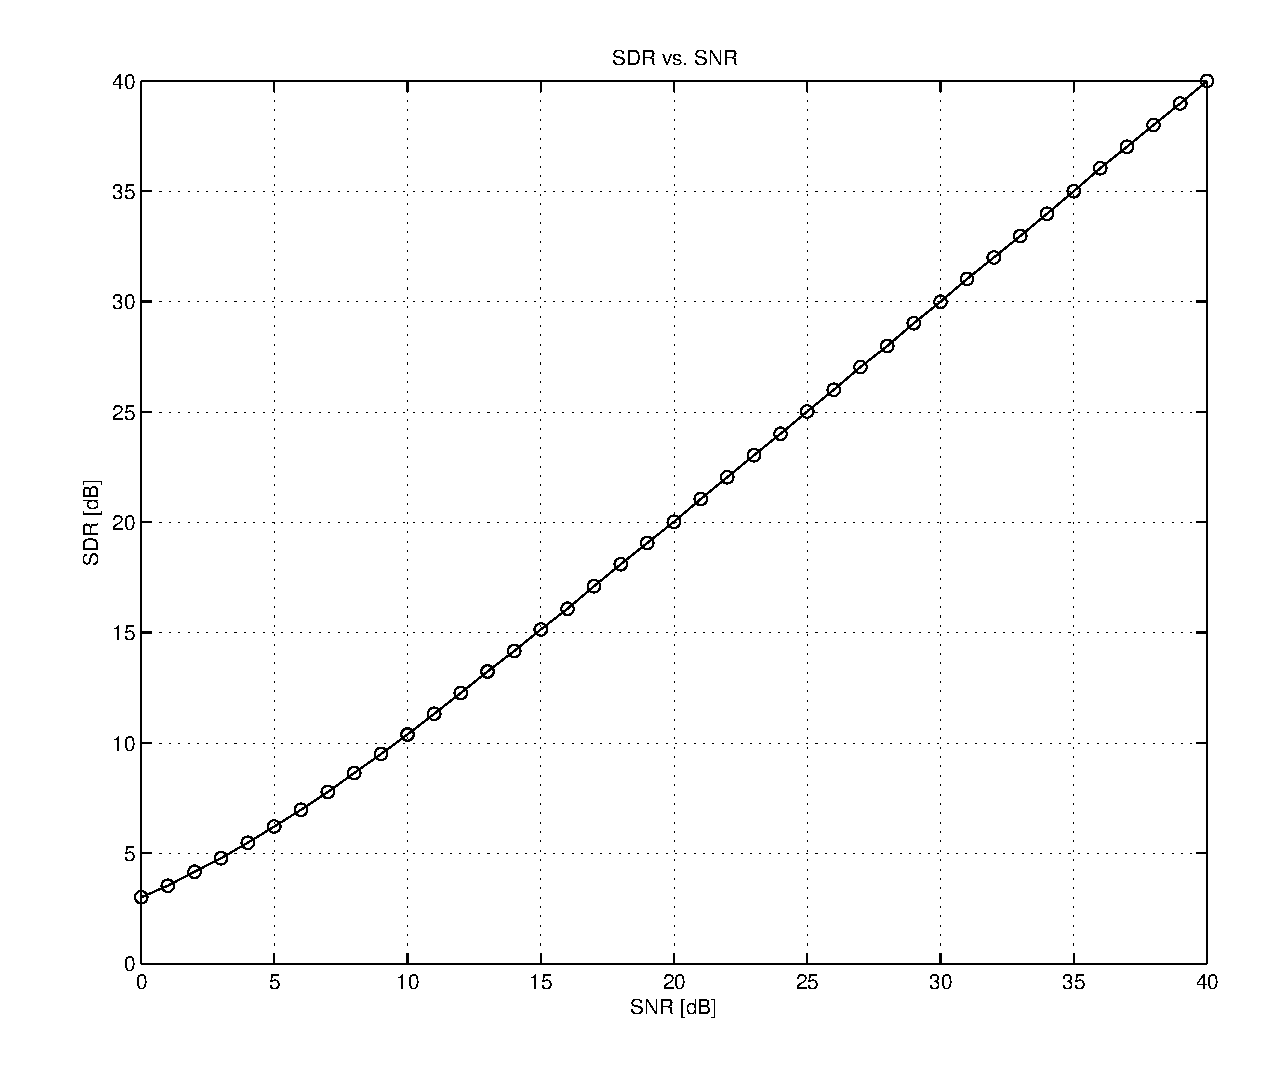
\includegraphics[width=\textwidth]{figures/matlab/ex_uncoded.pdf}
  \end{center}
  \caption{Plot of the SDR resulting from the \texttt{UncodedScheme} class,
  obtained using a \texttt{PerformanceProcessor}.}
  \label{fig:uncoded}
\end{figure}

This was not much work at all. Behind the scenes, however, a lot more was going
on:
\begin{enumerate}
  \item A long sequence of random source symbols was generated.
  \item For a range of SNR values and for each communication scheme, the source
    sequence was encoded using the |encode()| method of our new class,
    Gaussian noise of the appropriate variance was added, and the result was
    decoded using our new |decode()| method.
  \item The average difference between the source sequence and the estimate
    sequence was computed, again for each scheme and for each value of SNR. 
  \item The resulting performance curves were plotted by the
    |Performance|\-|Processor|.
\end{enumerate}
All this work was done by |Performance|\-|Processor| and the base class
|Practical|\-|Scheme|, leaving us free to focus on the essential stuff.
(\secref{impoverview} explains in detail how the above steps are performed.)


\subsubsection{Theoretical Performance}

At this point we have implemented uncoded communication, but we have not
yet verified that it performs indeed optimally. From \chapref{fundamentals} we know
that if there are $n$~channel uses per source symbol then the optimal SDR
is $(1 + \snr)^n$. In \jscsim\ we can implement this as a ``theoretical''
communication scheme: this is a communication scheme that doesn't actually do
any encoding or decoding, but simply computes a theoretical MSE for a 
given SNR.

\begin{listing}
\begin{Code}
  classdef ShannonScheme < TheoreticalScheme
    properties
      n         % The number of channel uses per source symbol.
    end

    methods (Access = 'public')
      function obj = ShannonScheme(sv, s, n)
        
        % Call base class constructor.
        obj = obj@TheoreticalScheme(sv, s);

        % Set class-specific parameters.
        obj.n = n;
      end
    end

    methods (Access = 'protected')
      % This function is called whenever the SNR is changed and so
      % the MSE needs to be recomputed.
      function update_mse(obj)
          obj.mse = obj.sv / (1 + obj.snr)^obj.n;
      end
    end
  end
\end{Code}
  \caption{A ``theoretical'' communication scheme does not perform any
  actual encoding or decoding, but rather computes the theoretically optimal MSE
  for a given SNR.}
  \label{lst:shannonscheme}
\end{listing}

The resulting \matlab\ code is given in \lstvref{shannonscheme}. We can make the
following observations.
\begin{enumerate}
  \item The class |ShannonScheme| is derived from |TheoreticalScheme| rather
    than from |PracticalScheme| as in the previous example (\lineref{1}). This
    is because unlike practical schemes, theoretical schemes do not have
    |encode()| or |decode()| methods. 
    
  \item |ShannonScheme| has a single parameter~|n|, the number of channel uses
    per source symbol, which it receives as an argument of its constructor
    (\lineref{7}).

  \item The method |update_mse(obj)| (\lineref{20}) is the heart of this
    class. This method is called by the base class whenever the SNR is
    changed. Here it computes $\ssq / (1
    + \snr)^n$, which is the theoretically optimal MSE for the given SNR
    (cf.~\chapref{fundamentals}).
    
  \item |update_mse()| accesses the |snr| property (\lineref{21}), even though
    we never defined this property. This is because the property is set by the
    base class, so that all derived classes have access to the SNR.
\end{enumerate}

To plot the performance of both |UncodedScheme| and |ShannonScheme| on the same
plot, we can use the |Performance|\-|Processor| as before:
\CodeInput{figures/matlab/ex_shannonscheme.minc}
The only difference to the previous example is that the |schemes| array now has
two elements and that we need to specify the parameter $n=1$ for
|ShannonScheme|.  This parameter will be passed to the constructor of
|ShannonScheme| as its third argument.

The resulting plot is shown on \figvref{shannonscheme}. Note that a legend has
automatically been added because we are plotting the performance of more than
one communication scheme.

\begin{figure}
  \begin{center}
    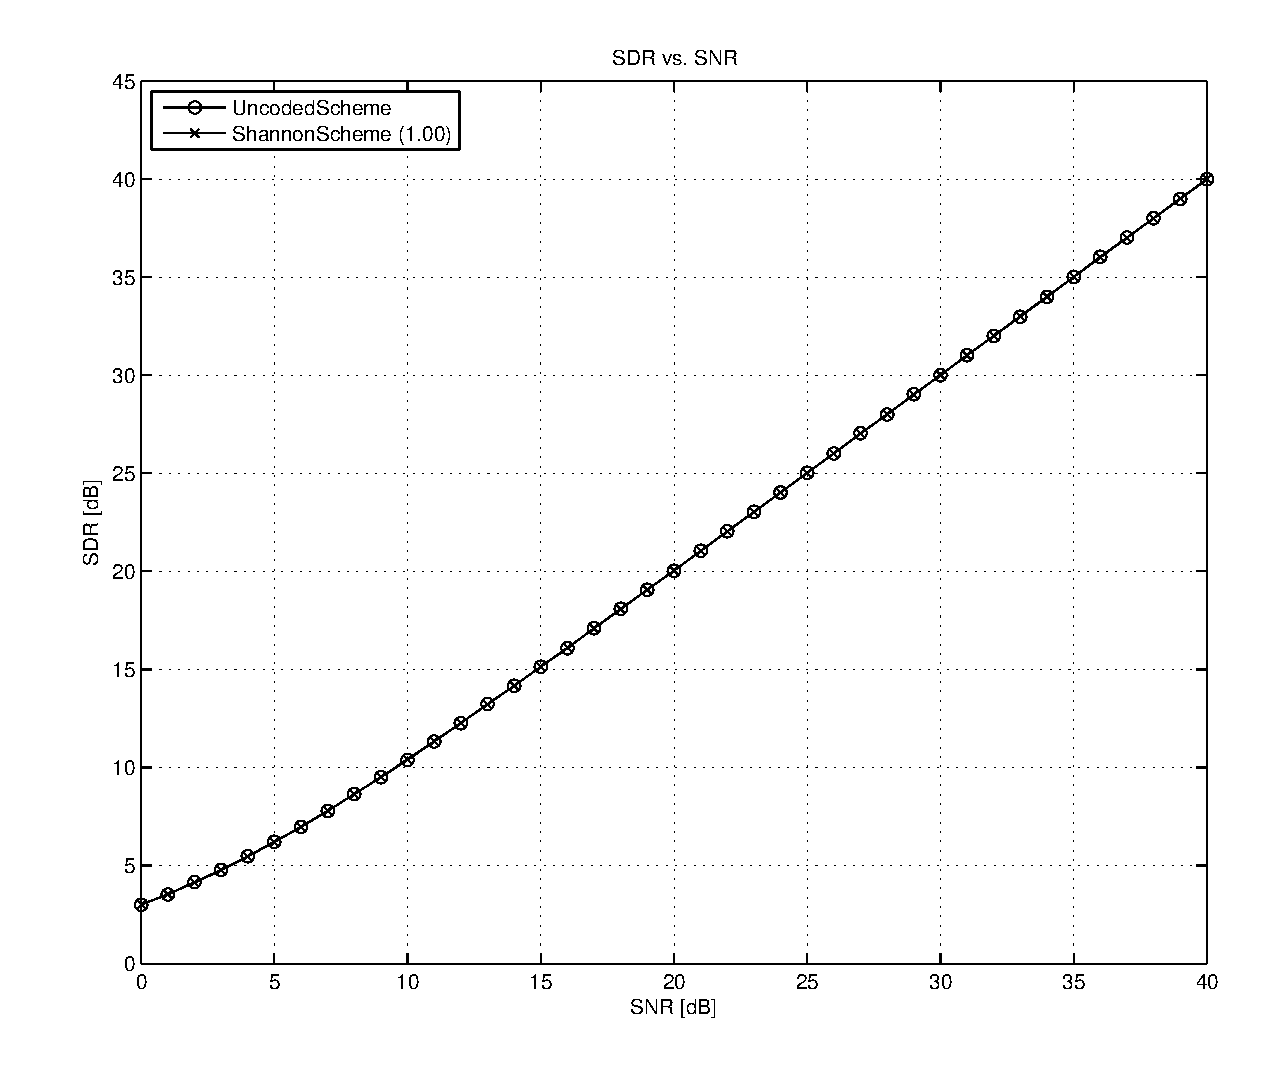
\includegraphics[width=\textwidth]{figures/matlab/ex_shannonscheme.pdf}
  \end{center}
  \caption{Comparing the theoretically optimal performance and the performance
  of uncoded transmission. The two curves coincide, experimentally confirming
  that uncoded transmission is optimal for the transmission of a Gaussian source
  across a Gaussian channel.}
  \label{fig:shannonscheme}
\end{figure}


\subsubsection{Alternative Output Formats}

In the examples we saw so far, the performance processor just launched a
standard \matlab\ figure window with the performance plot. Often, though, you
may not only want to look at the plot on the screen but also use it in a report
or in a paper. For this, \jscsim\ has the concept of \emph{output modules}. An
output module is a class that implements a rudimentary set of plot capabilities.

The default output module is called |MatlabPlotModule| and uses \matlab's plot
command to display a figure window. Alternatively, to save the performance plot
in a PDF file, for instance, the default output module can be replaced by a
|MatlabFilePlotModule|. Instead of displaying the plot in a window, this output
module saves it in a file.  Continuing our previous example, we can use it as
follows.
\begin{Code}
  ...  % Define list of schemes and parameters.
  pp = PerformanceProcessor();
  pp.output_module = MatlabFilePlotModule();
  pp.output_module.fn = 'myplot.pdf';
  pp.process(schemes, parameters);  % Saved to myplot.pdf.
\end{Code}
In \lineref{3} a new output module of type |MatlabFilePlotModule| is
created and attached to the performance processor. Since this output module
writes its output to a file, we have to specify a file name in \lineref{4}.
Afterwards, we can call |process()| just as before.\footnote{Unsurprisingly,
Figures~\ref{fig:uncoded} and~\ref{fig:shannonscheme} have in fact been created
using \Verb+Matlab+\-\Verb+FilePlotModule+.}

\urldef{\pgfplotsurl}\url{http://pgfplots.sourceforge.net/}
There is another output module, called |PGFPlotsOutputModule|. It produces a
file containing \LaTeX\ code to be used with the \pgfplots\
package\footnote{\pgfplotsurl}. To use it, just replace |MatlabFilePlotModule|
in the above example by |PGFPlotsOutputModule| and set \eg
\begin{Code}
  pp.output_module.fn = 'myplot.tex';
\end{Code}
The resulting file can then be included in a \LaTeX\ file, provided that the
|pgfplots| package has been loaded.  The result is shown on \figref{uncodedpgf}.
Admittedly, plots created by \pgfplots\ fit in nicer with the \LaTeX\
layout, and their labels are more readable than those of
Figures~\ref{fig:uncoded} and~\ref{fig:shannonscheme}.

\begin{figure}
  \begin{center}
    \input{figures/matlab/ex_uncodedpgf.tex_t}
  \end{center}
  \caption{Using the \texttt{PGFPlotsOutputModule}, one can save the simulation
  output as \TeX\ commands for the \pgfplots\ package, which can then be
  included in a \LaTeX\ source file.}
  \label{fig:uncodedpgf}
\end{figure}


\subsubsection{Analysis Using Scheme Processors}

The performance processor we have used to plot the performance in the previous
examples is a particular type of \emph{scheme processor}. The idea behind scheme
processors is to separate the implementation and the simulation of communication
schemes.

A scheme processor takes a list of schemes along with the corresponding
parameters, simulates these for a range of SNR values, and gathers data from
each simulation run. 

Each scheme processor is derived from the class |SchemeProcessor|. It must
implement three methods:
\begin{itemize}
  \item |initialize()| to allocate space for the data gathered;
  \item |save_scheme_data()| to collect data after each simulation run; and
  \item |post_process()| to post-process the gathered data, which usually just
    means to plot it.
\end{itemize}
This is illustrated by the simplified implementation of |PerformanceProcessor|
in \lstvref{perfproc}. This class has a single property, |mse| (\lineref{4}),
where it stores the mean squared errors gathered in each simulation run. In its
|initialize()| method, |mse| is initialized to a big all-zero matrix of the
right size. In the method |save_scheme_data()|, the communication scheme just
simulated (passed as the argument |scheme|) is queried by calling its
|compute_mse()| method (\lineref{13}) and the result is stored in the matrix
|mse|. Finally, |post_process()| plots the MSE of all processed schemes.

\begin{listing}
  \CodeInput{figures/matlab/PerformanceProcessor_ex.minc}
  \caption{Simplified implementation of the \texttt{PerformanceProcessor}
  class.}
  \label{lst:perfproc}
\end{listing}

For another example of a performance processor, consider the hybrid
communication scheme implemented as |Hybrid2DScheme| in \lstref{hybridscheme}.
In this communication scheme, each source symbol~$S$ is split into a discrete
part~$Q$ and a continuous part~$E$ (lines~10--11), which are then transmitted
across two
channel uses (lines~13--14).  The decoder computes the source estimate~$\Sh$
from the separate estimates~$\Qh$ and~$\Eh$ (lines 18--20). (This is similar to
the communication schemes introduced in \chapref{mindelbwex}.)

\begin{listing}
\begin{Code}
  classdef Hybrid2DScheme < PracticalScheme
      
      properties (Access = 'protected')
          q
          qh
      end
      
      methods (Access = 'protected')
          function x = encode(obj, s)
              obj.q = discrete_part(s);
              e = continuous_part(s);
              
              x(1, :) = scale_to_power_constraint(obj.q);
              x(2, :) = scale_to_power_constraint(e);
          end
          
          function sh = decode(obj, y)
              obj.qh = estimate_qh(y);
              eh = estimate_eh(y);
              sh = combine_estimates(obj.qh, eh);
          end

          % Other methods here ...
      end

      % Methods for scheme processors to access simulation data.
      methods (Access = 'public')
          function q = compute_q(obj)
              q = obj.q;
          end
          
          function qh = compute_qh(obj)
              qh = obj.qh;
          end
      end
  end
\end{Code}
\caption{Simplified implementation of a hybrid communication scheme. Note how
\texttt{qh} and \texttt{eh} are saved as class properties, so that they can be
accessed by a scheme processor through the respective \texttt{compute\_*}
methods.}
\label{lst:hybridscheme}
\end{listing}

A question of interest is the behavior of the average error $\E[(Q - \Qh)^2]$ as
a function of the SNR. The scheme processor |Hybrid2DProcessor| in
\lstref{hybridprocessor} solves this task in a few small steps. It is very
similar to the |PerformanceProcessor| of \lstref{perfproc}, except that
different variables are accessed in \lineref{13}. Since the corresponding
communication scheme class, |Hybrid2DScheme|, saves |q| and~|qh| as class
properties and implements public |compute_*| methods for these properties,
the |save_scheme_data()| method of the new scheme processor can easily access
these and compute the corresponding error.

\begin{listing}
\begin{Code}
  classdef Hybrid2DProcessor < SchemeProcessor
      
      properties (Access = 'protected')
          qe
      end
      
      methods (Access = 'protected')
          function initialize(obj)
              obj.qe = zeros(obj.nb_schemes(), length(obj.snr));
          end
          
          function save_scheme_data(obj, scheme, j, k)
              obj.qe(j, k) = mean((scheme.compute_q() - ...
                scheme.compute_qh()).^2);
          end
          
          function post_process(obj)
              % Plot qe vs. SNR ...
          end
      end
  end
\end{Code}
\caption{A scheme processor to plot the estimation error of the discrete part in
a hybrid communication scheme.}
\label{lst:hybridprocessor}
\end{listing}


\subsection{Implementation Overview}\label{sec:impoverview}

\subsubsection{Design Philosophy}

The design philosophy behind \jscsim\ is to separate the implementation of a
communication strategy and the simulation thereof. The end user should be able
to concentrate either on implementing the communication scheme or writing the
code that processes it during simulation, but shouldn't have to think about both
tasks at the same time.  For this reason, the core classes that make up \jscsim\
are divided into two categories. In the first category are the \emph{scheme
classes} (or simply 'schemes'), which are classes that implement communication
schemes and have the class |Scheme| as their common ancestor. \secref{ooforsim}
already covered why it makes sense to implement communication schemes as
classes. 

The second category consists of  \emph{scheme processors}, which are classes
that implement the processing of a particular quantity (such as the MSE) during
the simulation of a single or of a family of communication schemes. Scheme
processors derive from the common ancestor class |SchemeProcessor|. What is the
motivation behind organizing the processing code in this way? The ``processing''
of a communication scheme consists of two steps:
\begin{enumerate}
  \item simulating the scheme by feeding the encoder with randomly generated
    source samples, transforming the encoder output by simulating a noisy
    channel (\eg, by adding Gaussian noise), and passing the channel output to
    the decoder
  \item gathering relevant data, \eg, the mean squared error or other
    performance criteria, after the simulation has run, and displaying it
\end{enumerate}
The base class |SchemeProcessor| essentially implements the first
step.\footnote{To be exact, as this section will explain, some of the simulation
code is actually in the class \texttt{PracticalScheme}.} The
second step is implemented in derived classes such as
|Performance|\-|Processor| (which computes and plots the achieved SDR). This
structure makes it possible to quickly implement new processor classes to
analyze arbitrary quantities of a communication scheme or of a set of schemes,
as the examples in the previous section show.

Based on the reasonable assumption that you implement a particular
communication scheme in \jscsim\ because you eventually want to simulate it, you never directly instantiate a scheme class. Rather, you create a
particular scheme processor (by instantiating a class derived -- directly or
indirectly -- from |SchemeProcessor|) and call its |process()| method. Note that
you cannot create an instance of the base class |SchemeProcessor| since the
latter contains abstract methods\footnote{An \emph{abstract method} is a
method that is declared in a class but not implemented. For example, a class
\texttt{Shape} may declare an abstract method \texttt{compute\_area()}, which
must be implemented by the derived classes \texttt{Circle}, \texttt{Square}, and
\texttt{Triangle}. A class that has abstract methods cannot be instantiated.}
and serves only as a template for scheme processors. The
example on page~\pageref{sec:perfanalysis} shows how a performance processor,
which is a particular type of scheme processor, is used to plot the
SDR achieved by a communication scheme.

The interaction between scheme processors and scheme classes is illustrated in
\figvref{schemeprocinteraction}.  When you first create an instance of a scheme
processor, it generates and saves a random source sequence of a default
variance.\footnote{By default, the source samples are normally distributed, but
this behavior may easily be changed by a derived class.} Next you call the
|process()| method of the scheme processor, passing a list of schemes (\ie,
names of scheme classes) and a list of parameters for each scheme (cf.~the
example on page~\pageref{sec:perfanalysis}). (A scheme can have any number of
parameters, like for instance the number of channel input symbols produced per
source symbol.) Internally, the scheme processor then creates an instance of
each specified scheme, passing the source sample sequence to each one's
constructor. Because all schemes operate on the same source sequence, a fair
comparison is guaranteed. 

\begin{figure}
  \begin{center}
    \input{figures/schemeprocessor.tex_t}
  \end{center}
  \caption{Interaction between a scheme processor and scheme classes. For each
  scheme, the scheme processor repeatedly calls the scheme's \texttt{set\_snr()}
  method with different SNR values and then gathers the resulting simulation
  data.}
  \label{fig:schemeprocinteraction}
\end{figure}

A scheme processor has a list of SNR values for which each scheme is to be
processed. By default, it runs from 0dB to 40dB with increments of~1dB. For
each SNR value and for each scheme, the scheme processor calls the scheme's
|set_snr()| method, passing the SNR value as an argument (cf.~\lineref{13} in
\lstvref{schemeclass}). 

When a scheme's |set_snr()| method is called, it stores the new SNR in its |snr|
property and calls the |snr_updated()| method. The job of this method is to
update the state of the scheme object to reflect the new SNR. For example, after
a call to a scheme object's |set_snr()| method, its |mse| property should be set
to the mean square error that the scheme achieves with the given SNR. How
exactly a scheme updates its state when |snr_updated()| is called is up to the
implementation. As we will see below, though, the procedure is very similar for
a large class of schemes, of which \jscsim\ takes advantage. 

After calling a scheme's |set_snr()| method, a scheme processor can access
the scheme's |mse| property (for instance) via the scheme's |compute_mse()|
method (which we will see shortly). A scheme processor whose purpose it is to
track the MSE achieved by a particular scheme thus alternatingly calls
|set_snr()| and |compute_mse()| and stores the MSE for each SNR. This is
precisely what the class |PerformanceProcessor| does. 

Other scheme processors collect different data. For instance, the
|Hybrid2DProcessor| in \lstvref{hybridprocessor} separately computes and stores
the errors from the discrete and the continuous transmission rounds for the
hybrid scheme in \lstref{hybridscheme}.

The remainder of this section looks in detail at the implementation of the
scheme classes and of the performance processors.


\subsubsection{Scheme Classes}

The common ancestor of all scheme classes is called |Scheme| and is shown in
\lstvref{schemeclass}. It defines the most rudimentary features that all
communication scheme implementations must have. 

\begin{listing}
\CodeInput{figures/matlab/Scheme.minc}
\caption{The \texttt{Scheme} class is the base class from which all
communication scheme classes are derived.}
\label{lst:schemeclass}
\end{listing}

The class definition starts in \lineref{1}. It is a \matlab\ convention that any
class whose internal state can change over time (as is the case for all classes
considered here) must be derived from the |handle| class, but this is only a
technical detail and of no importance in the sequel.

As we will shortly see in detail, \jscsim\ divides communication schemes into
two types: theoretical schemes and practical schemes. Schemes of both
types are (indirectly) derived from |Scheme|, so |Scheme| defines only the
behavior common to both types, which consists essentially of the methods to set
the SNR and to retrieve the MSE. 

Every communication scheme has access to the three properties defined in
lines~2 to~6: the source variance, the SNR, and the incurred mean squared error.
The source variance is passed via the constructor whenever a class derived from
|Scheme| is instantiated (\lineref{9}). The SNR is set by |set_snr()|
(\lineref{13}). The MSE property is not set by any of the class' methods; it
will be the job of the derived classes to update this property in their
|snr_updated()| method. 

You may wonder why the constructor in \lineref{9} receives an argument~|s| but
ignores it. The reason is that a scheme processor always passes the list of
source symbols to a scheme it processes, even if it is a theoretical scheme that
does not use the source symbols. More about this is explained further below.

We have already mentioned the method |set_snr()| (\lineref{13}). It is called by
a scheme processor whenever the communication scheme is to be simulated for a
new SNR. This method first saves the new SNR in its |snr| property
(\lineref{14}) and then calls the abstract method |snr_updated()| to inform
derived classes about the changed SNR.

The method |compute_mse()| allows scheme processors to access a scheme's
|mse| property. (Because the property is declared as \emph{protected} (cf.
\lineref{2}), it cannot be directly accessed from outside the class, only
through a method.) 

Line~24 declares the abstract method |snr_updated()|. Because |Scheme| itself
does not implement this method, the class cannot be instantiated directly.
Instead, any class derived from |Scheme| must implement
|snr_updated()|.\footnote{It is not quite true to say that any class derived
from \texttt{Scheme} \emph{must} implement the abstract method
\texttt{snr\_updated()}. A derived class is free not to implement the method; if
it does not implement it, however, it remains itself an abstract class and
cannot be instantiated either. A class can only be instantiated if it implements
all abstract methods defined by any of its ancestors. Of course, if a base class
\texttt{X} has already implemented an abstract class, then other classes derived
from~\texttt{X} no longer need to implement the abstract method themselves as
they inherit the implementation from~\texttt{X}.}


\subsubsection{Theoretical Schemes}

Theoretical schemes could also be called ``virtual'' schemes. They are not
actual communication strategies, they rather compute theoretical values for a
given SNR. The purpose of a theoretical scheme is to compare the behavior of a
communication scheme to a theoretically expected behavior. For an example, see
the class |ShannonScheme| in \lstvref{shannonscheme}.

The implementation of |TheoreticalScheme| is given in
\lstvref{theoreticalscheme}. The class directly derives from |Scheme|
(\lineref{1}); its constructor does nothing except call the base class
constructor, passing on the arguments (\lineref{4}). 

\begin{listing}
  \CodeInput{figures/matlab/TheoreticalScheme.minc}
  \caption{Simplified implementation of the class \texttt{TheoreticalScheme}.}
  \label{lst:theoreticalscheme}
\end{listing}

As mentioned before, classes derived from |Scheme| must implement the method
|snr_updated()|. The implementation in |TheoreticalScheme| is quite simple:
|snr_updated()| just calls |update_mse()|. The latter is itself an abstract
method of |TheoreticalScheme|. This way of structuring the class is just a
programmatical way of saying ``the only thing a theoretical scheme needs to do
when a new SNR is set is to compute the MSE as a function of the SNR''.
Listing~\ref{lst:shannonscheme} provides a sample implementation of
|compute_mse()|. 


\subsubsection{Practical Schemes}

As opposed to theoretical schemes, practical schemes are classes that actually
\emph{implement} a communication scheme. When the SNR is updated, a practical
scheme must simulate encoding, transmission, and decoding of the source symbols.
Since this procedure (except the particularities of encoding and decoding) is
the same for all practical schemes, it is implemented in the class
|PracticalScheme|, from which implementations of particular communication
schemes can then be derived. The actual encoding and decoding functions are
declared abstract in |PracticalScheme|, \ie, classes that implement
communication strategies need only implement these two methods. 

A simplified version of |PracticalScheme| is shown in \lstvref{practicalscheme}.
Its |snr_updated()| method performs exactly the steps mentioned above: the
source sequence~|s| is encoded into a channel input sequence~|x| (\lineref{5}),
transmission is simulated by adding Gaussian noise to~|x| (\lineref{8}), and
the channel output~|y| is decoded to yield the estimate sequence~|sh|
(\lineref{11}).  Finally, the MSE is computed and stored in the |mse|~property
(\lineref{14}).  This is the precisely the property that a performance processor
accesses when it calls the scheme's |compute_mse()| method (which we saw in the
base class |Scheme|). 

\begin{listing}
  \CodeInput{figures/matlab/PracticalScheme.minc}
  \caption{A simplified implementation of \texttt{PracticalScheme}. The methods
  \texttt{encode()} and \texttt{decode()} are declared abstract and must be
  implemented by derived classes.}
  \label{lst:practicalscheme}
\end{listing}

The methods |encode()| and |decode()| are the defining feature of a
communication scheme. There is no ``default'' encoder and decoder, hence
|PracticalScheme| does not provide an implementation of them but declares them
as abstract. They must be implemented by derived classes (such as
|UncodedScheme| in \lstvref{uncoded}).


\subsubsection{Scheme Processors}

Scheme processors instantiate a list of scheme classes and process them for a
range of SNR values. All scheme processors derive from |SchemeProcessor|, a
simplified implementation of which is given in \lstvref{schemeprocessor}. 

\begin{listing}
  \CodeInput{figures/matlab/SchemeProcessor.minc}
  \caption{Simplified implementation of the \texttt{SchemeProcessor} class.}
  \label{lst:schemeprocessor}
\end{listing}

All scheme processors have at the three properties defined in lines~3--5. The
vector~|s| stores the source sequence, which is created in the constructor upon
instantiation (\lineref{16}). The other two properties, |schemes| and
|parameters|, hold the list of schemes to process and the corresponding
parameters, respectively. 

|SchemeProcessor| also has three \emph{public} properties. Because they are
declared \emph{public}, they can be changed from outside the class; they allow
the user of a scheme processor to control the latter's behavior. The meaning of
these three properties should be self-evident from the code; for details see
\secref{reference}.

A scheme processor is launched by calling its |process()| method. This method
has two arguments, |schemes| and |parameters|. Both are cell arrays that
specify the schemes to be processed (\ie, the names of the respective classes)
and the parameters for each scheme, respectively. See
page~\pageref{sec:perfanalysis} for an example of how to call |process()|.

|process()| first saves the schemes and parameters in the respective class
properties (\lineref{20} resp.~lines~4--5). Then it calls the |initialize()|
method (\lineref{21}). This abstract method allows scheme processor
implementations to do things before the actual processing starts. The most
common use of this function is to allocate a data structure that will hold the
data gathered from the schemes (for an example, see the implementation of
|PerformanceProcessor| in \lstvref{perfproc}).  The |do_processing()| method
(line~22 resp.~28) then performs the actual processing of the schemes, we will
look at it in detail shortly. Finally, the abstract method |post_process()| is
called (\lineref{23}). In this method, derived classes can for example display
the data gathered from the schemes, or save it in a file, etc.

The function |do_processing()|, which starts in \lineref{28}, is the core of
|SchemeProcessor|. In two nested \emph{for} loops it traverses the list of
schemes and the range of SNR values. For each scheme and for each SNR it first
calls |set_snr()| (we have already seen above what this method does), and then
it calls the abstract method |save_scheme_data()| (\lineref{35}). In their
implementation of this key method, derived classes determine which data to save
about the scheme. For example, the performance processor on
page~\pageref{sec:perfanalysis} uses it to store the MSE. (The arguments of
|save_scheme_data()| are described in detail in \secref{reference}.)


\subsubsection{Summary}

The preceding paragraphs have hopefully given the reader a good overview of how
\jscsim\ is implemented. Naturally, some details have been swept under the rug.
For instance, |PracticalScheme| also helps in arranging the source sequence in
blocks of $k$~source symbols if a scheme encodes more than one source symbol at
once, and scheme processors use a slightly more involved method to store schemes
and their parameters internally than the one shown. For these details, the
reader so inclined is invited to peruse the source code.


\section{Reference}\label{sec:reference}

This reference section explains in detail how to use \jscsim\ to implement new
communication schemes, how to simulate them, and how to build custom scheme
processors. 


\subsection{Communication Schemes}

There are two kinds of communication schemes in \jscsim: \emph{theoretical}
schemes and \emph{practical} schemes. Theoretical schemes compute the MSE for a
given SNR by computing some function of it without simulating anything. They
allow you to compare the performance of a particular communication scheme with a
theoretical value, as for example the |ShannonScheme| in \lstref{shannonscheme}.
On the other hand, practical schemes (like the one in \lstref{uncoded})
determine the MSE by actually simulating communication.


\subsubsection{Theoretical Schemes}

Theoretical communication schemes are implemented as classes derived from
|TheoreticalScheme|. Any class derived from |TheoreticalScheme| must implement
the following methods.

\begin{method}{\meta{class name}(\oarg{sv}, \oarg{s}
  [, \opt{\meta{parameters}}]) (public)}
  This is the constructor of the class. The first two arguments are the source
  variance +sv+ and the source sample sequence~+sv+, which must be passed on to
  the base class constructor, \ie, by calling
  \begin{Code}
  obj@TheoreticalScheme(sv, s);
  \end{Code}

  If a theoretical scheme has parameters, such as the bandwidth expansion
  factor~|n| of |ShannonScheme| (cf.~\lstref{shannonscheme}), they must be
  specified as additional arguments to the constructor.
\end{method}

\begin{method}{update_mse(\obj) (protected)}
    This method is called by the base class whenever the SNR is changed. It
    must update the |mse| property based on the value of the |snr| property.
    For example, the |update_mse()| method of |ShannonScheme| sets |mse| to be
    $\ssq / (1 \normalplus \snr)^n$.
\end{method}


\subsubsection{Practical Schemes}

Practical communication schemes are implemented as classes derived from
|PracticalScheme|. Any class derived from |PracticalScheme| must implement the
following methods.
\begin{method}{\meta{class name}(\oarg{sv}, \oarg{s}
  [, \opt{\meta{parameters}}]) (public)}
  This is the constructor of the class. The first two arguments are the source
  variance +sv+ and the source sample sequence +s+, which must be passed on to
  the base class constructor. The base class constructor has two more arguments,
  which are the number $k$~of source symbols encoded at a time, and the number
  $n$~of channel symbols produced for every $k$~source symbols.
  Depending on the scheme, these can be fixed values (as in |UncodedScheme| in
  \lstref{uncoded}) or variable parameters of the scheme itself.

  \codeexample A scheme that only works for $1$:$2$ bandwidth expansion would
  have a constructor similar to the following.
  \begin{Code}
  function obj = MyScheme1(sv, s)
    obj@PracticalScheme(sv, s, 1, 2);
    % rest of constructor ...
  end
  \end{Code}
  On the other hand, a scheme that encodes one source symbol into $n$~channel
  inputs, where $n$~is arbitrary, would define a constructor like this.
  \begin{Code}
  function obj = MyScheme2(sv, s, n)
    obj@PracticalScheme(sv, s, 1, n);
    % rest of constructor ...
  end
  \end{Code}
\end{method}

\begin{method}{\oarg{x} = encode(\obj, \oarg{s}) (protected)}
  This method receives +s+, a matrix of source samples with $k$~rows, and must
  return a matrix~+x+ with $n$~rows and the same number of columns as~+s+.
\end{method}

\begin{method}{\oarg{sh} = decode(\obj, \oarg{y}) (protected)}
  This method receives the channel output~+y+ as a matrix with $n$~rows and
  must return a matrix~+sh+ with $k$~rows of source estimates
\end{method}

In addition, derived classes may want to override
|update_variable_parameters()|.
\begin{method}{update_variable_parameters(\obj) (protected)}
  In this method, which is called whenever the SNR changes, derived classes can
  update any of their own properties that depend on the SNR. It
  is important that if a derived class overrides this method, it must first
  call the base class method, \ie,
  \begin{Code}
  function update_variable_parameters_(obj)
    % Call base class version.
    update_variable_parameters@PracticalScheme(obj); 
    % Your code here ...
  end
  \end{Code}
\end{method}

To allow a scheme processor to track a particular property of a communication
scheme, the property must be made accessible. This is normally done by  writing
a |compute_*| method. We have already seen the example of the |compute_mse()|
function, which is defined by the class |Scheme|. The class |PracticalScheme| in
addition implements the following such methods.

\begin{method}{x = compute_x(\obj) (public)}
  Returns the channel input sequence.
\end{method}

\begin{method}{y = compute_y(\obj) (public)}
  Returns the channel output sequence.
\end{method}

\begin{method}{sh = compute_sh(\obj) (public)}
  Returns the sequence of source estimates.
\end{method}

Any derived class must thus implement a |compute_*| function for each
property it wants to make accessible to a scheme processor.


\subsection{Scheme Processors}

Scheme classes are usually not handled directly; rather, they are processed by
a \emph{scheme processor}. Scheme processors evaluate a set of communication
schemes for a range of SNR values and store and process the data gathered during
the simulations.

All scheme processors are implemented as classes derived from |SchemeProcessor|.
To process a communication scheme (or a set of schemes) you never directly use a
|SchemeProcessor| object. Instead, you either use an existing derived class such
as |PerformanceProcessor|, or you implement a custom scheme processor. 


\subsubsection{General Aspects}

The behavior of all scheme processors can be controlled through the following
properties, defined in the class |SchemeProcessor|.
\begin{property}{snr (public; default ?10.^(0:.1:4)?)}
  A vector that specifies the SNR range over which the
  communication schemes are simulated. By default it is set to the range
  0dB to 40dB with increments of 1dB. 
\end{property}

\begin{property}{N (public; default ?100000?)}
  The length of the random source sample sequence.
\end{property}
  
\begin{property}{verbose (public; default ?false?)}
  If this parameter is set to true, various status and debugging messages are
  displayed during the simulations.
\end{property}

\begin{property}{output_module (public)}
  This is the output module used by the scheme processor to display its
  results (see the section on output modules). The default output module is
  |MatlabPlotModule|.
\end{property}

\begin{property}{legendmode (public, default \texttt{'auto'})}
  This property determines the behavior of the |plot_vs_csnr()| and
  |plot_|\-|vs_|\-|csnr_|\-|db()| functions (cf.~the definition of |post_process()| below).
  If |legendmode| is set to |'on'|, a legend is always displayed. If it is set
  to |'off'|, a legend is never displayed. If it is set to |'auto'|, a legend is
  only displayed if more than one scheme is plotted.
\end{property}

All scheme processors are launched using the |process()| method.
\begin{method}{process(\obj, \oarg{schemes}, \oarg{parameters}) (public)}
  Process the specified schemes for the specified parameters. The cell array
  +schemes+ lists the schemes to be processed; each of its elements is a string
  equal to the name of a scheme class.

  The cell array +parameters+ has the same number of elements as +schemes+. For
  a scheme that does not have any parameters, the corresponding entry of
  +parameters+ must be an empty matrix.  For a scheme that accepts
  $m$~parameters (\ie, its constructor has $m$ arguments other than |sv| and
  |s|), the corresponding entry of +parameters+ must be a matrix with
  $m$~rows; the scheme is then processed once for each
  column of the matrix, using the parameters from the respective column.
  This makes it easy to use \matlab's colon operator (|:|) to specify a
  \emph{range} of parameters.
  \codeexample Suppose |process()| is called as follows.
  \begin{Code}
  pp = PerformanceProcessor();
  pp.process({'MyScheme'}, {[1:4; 0.1:0.1:0.4]});
  \end{Code}
  Then |MyScheme| will be processed 4~times: once with the parameters $1$
  and~$0.1$, once with the parameters $2$ and~$0.2$, and so on. \Ie, \lineref{2}
  above has the same effect as
  \begin{Code}
  pp.process({'MyScheme', 'MyScheme', 'MyScheme', 'MyScheme'}, ...
    {[1;0.1], [2;0.2], [3;0.3], [4;0.4]});
  \end{Code}

  Internally, a scheme is counted as many number of times as its parameter
  matrix has columns. This means that for the above example, |nb_schemes()|
  (cf.~below) returns~$4$.

\end{method}


\subsubsection{The Performance Processor}

This is the only scheme processor that is already implemented in \jscsim. It
works for all communication schemes derived from |Scheme|. It simply plots the
SDR vs SNR curve of the specified communication scheme, as illustrated by the
examples in \secref{tutorial}.

To have fine grained control over the plot of the simulation results, the plot
functionality of a performance processor can be disabled by setting its
|output_module| property to the empty matrix\footnote{or
any other value for which \matlab's \texttt{isempty()} function returns
\texttt{true}, such as the empty string~\texttt{''}, the empty
cell~\texttt{\char`\{\char`\}}, etc.}. The simulation results can then be read
from the performance processor's |mse| property, which is declared |public|, and
plotted with a custom output module. This is the recommended strategy if you
want to manually specify say the plot legend or the axis labels, as illustrated
by the example in \lstref{customppplot}. For this reason, it is also recommended
that custom scheme processors (see the following paragraph) declare their
simulation results data as |public|. 

\secref{outputmodules} has a detailed description of output modules.

\begin{listing}
\begin{Code}
  pp = PerformanceProcessor();
  pp.output_module = [];  % Disable built-in output module.
  pp.process({'ShannonScheme', 'UncodedScheme'}, {1, []});

  % Create own output module.
  om = MatlabPlotModule();

  % Access SNR and simulation result from PerformanceProcessor object.
  om.x = 10*log10(pp.snr);  % converted to dB
  om.y = 10*log10(pp.sv ./ pp.mse);  % SDR = source variance / mse

  % Set custom labels, legend, etc.
  om.legend = {'theoretical limit', 'uncoded communication'};
  % ...

  % Display plot.
  om.do_plot();
\end{Code}
\caption{This example shows how the internal output module of a performance
processor can be disabled and the simulation results can be plotted on a custom
plot.}
\label{lst:customppplot}
\end{listing}


\subsubsection{Implementing a New Scheme Processor}

Custom scheme processors are implemented by creating a new class derived from
|SchemeProcessor|. Such a class must implement the three following methods.

\begin{method}{initialize(\obj) (protected)}
  This method is called before the actual processing starts. It can be used \eg\
  to allocate data structures to save simulation data.

  |SchemeProcessor| provides the useful helper function |nb_schemes()|, which
  returns the number of schemes that have been passed to |process()|. In
  addition, |length(obj.snr)| gives you the number of values in the SNR range.
\end{method}

\begin{method}{save_scheme_data(\obj, \oarg{scheme}, \oarg{j}, \oarg{k})
  (protected)}
  This method is called each time a scheme has been processed for a particular
  SNR and gives you the opportunity to save data about the simulation run.
  +scheme+ is the scheme object that was just run; you can gather data about it
  by calling its public methods. For example, the |save_scheme_data()| method
  of |PerformanceProcessor| calls the |compute_mse()| method of +scheme+ to
  store the MSE.

  +j+ is a number between~$1$ and |nb_schemes()| and +k+ is a number between~$1$
  and |length(obj.snr)|; they refer to the current scheme and the current SNR
  value, respectively. \lstref{perfproc} shows a typical example of how they are
  used.
\end{method}

\begin{method}{post_process(\obj) (protected)}
  This method is called after all schemes have been processed. Here you can post
  process the data gathered by |save_scheme_data()|, for instance by plotting
  it.

  |SchemeProcessor| provides the helper function |plot_vs_snr(obj, m)|, which
  plots the data in the vector |m| against the SNR in dB. (The SNR is in dB, not
  the data; if you also want the data to be plotted on a dB scale, use
  |plot_vs_snr_db()| instead.)
\end{method}

To change the default output module, override the following method.
\begin{method}{\oarg{om} = default_output_module(\obj) (protected)}
  This method is called by the constructor of |SchemeProcessor| to install the
  default output module. 
\end{method}

In addition, a custom scheme processor can override
|create_|\-|source_|\-|samples()| to change the source distribution.

\begin{method}{s = create_source_samples(\obj) (protected)}
  This method must return a sequence of |N| independent random source samples of
  variance~|sv|. The default implementation in |SchemeProcessor| creates
  Gaussian source samples.
\end{method}


\subsection{Output Modules}\label{sec:outputmodules}

In some cases you might just want to see the results of a simulation on screen;
in other cases you might want to save them in a file that you can include in a
paper or report. In \jscsim\ it is easy to change the default behavior by
changing the output module.

Output modules provide an abstraction of basic plot functionalities. You can
think of them as a kind of output ``plugins''. The functionality they offer is
rather orthogonal to the task of simulating; they may well be used in other
programs as well. 

In \jscsim, each class derived from |SchemeProcessor| has an output module
associated to it. By default this is the |MatlabPlotModule|, which displays the
plots in a regular \matlab\ figure window, but it is easy to change the plot
module in order to save the plot in a PDF file rather than on screen, for
instance:
\begin{Code}
  pp = PerformanceProcessor();
  pp.output_module = MatlabFilePlotModule();
  pp.output_module.fn = 'myplot.pdf';
\end{Code}

The behavior of output modules is controlled by a set of parameters. Some of
these, such as the axis labels or the legend entries, apply to all
output modules. Other parameters apply only to certain categories of output
modules: the |fn| property, for instance, which determines the name of the file
in which to save a plot, only applies to those output modules that can save
plots in a file. 


\subsubsection{General Parameters}

All output modules support the following properties and methods.
\begin{property}{x (public)}
  The range of $x$~values. This must be a row vector.
\end{property}
\begin{property}{y (public)}
  The data to plot against the $x$~values. This must be either
  a row vector or a matrix with the same number of columns as~|x|; each
  row then corresponds to a separate data series to plot.
\end{property}

\begin{property}{xlabel (public)}
  The label of the $x$-axis. This is a string; it can
  also contain (limited) \LaTeX\ code depending on the actual output module
  used. 
\end{property}
\begin{property}{ylabel (public)}
  The label of the $y$-axis. This is a string; it can
  also contain (limited) \LaTeX\ code depending on the actual output module
  used.
\end{property}

\begin{property}{plottitle (public)}
  The plot title. This is a string; it can also
  contain (limited) \LaTeX\ code depending on the actual output module used.
\end{property}

\begin{property}{legend (public)}
  The legend entries. This must be a cell array of
  strings. If the number of legend entries is smaller than the number of data
  series in~|y|, a warning is issued.
\end{property}

\begin{property}{legendpos (public)}
  A string determining where in the plot the legend is
  placed. The possible values are |NorthEast|, |NorthWest|, |SouthEast|,
  |SouthWest|, and |NorthEast|\-|Outside|. If |legendpos| is set to
  the empty string, no legend is created.
\end{property}

\begin{property}{grid (public; default ?false?)}
  This boolean parameter determines whether a grid is drawn (if set to |true|)
  or not (if set to |false|).
\end{property}

\begin{method}{set_color_mode(\obj, \oarg{c}) (public)}
  Set the color mode of the plot. +c+ can either be |'color'|, in which case a
  line of a different color is drawn for each data series, or |'bw'|, in which
  case the plot uses black lines with a different marker for each data series.
\end{method}

To use an output module on its own, \ie, outside of a scheme processor, call the
|do_plot()| method.
\begin{method}{do_plot(\obj) (public)}
  Plots the data set specified by~|x| and~|y|.
\end{method}


\subsubsection{The MatlabPlotModule Output Module}

This output module creates a standard \matlab\ plot. It is the default output
module for scheme processors. It has a single public property.
\begin{property}{ah (public)}
  A handle to the axes that will contain the plot. By default,
  |Mat|\-|lab|\-|Plot|\-|Mod|\-|ule| creates a new figure window and sets |ah|
  to point to the axes of the new windows. You can have |MatlabPlotModule| to
  plot on an existing set of axes by changing the |ah| property. 
    
  \codeexample To create the plot in a subplot of an existing figure window:
\begin{Code}
  figure;
  ah1 = subplot(2,1,1);
  pp = PerformanceProcessor();
  pp.output_module.ah = ah1;
\end{Code}
  Subsequent plots now appear in the specified subplot.
\end{property}


\subsubsection{The MatlabFilePlotModule Output Module}

The |MatlabFilePlotModule| works just like the |MatlabPlotModule|, except that
the plot is not displayed in a window but saved in a file. The result is the
same as if you had selected ``File\slash Save~as...'' in a figure window. 

The behavior of |MatlabFilePlotModule| is controlled by the following
properties.
\begin{property}{fn (public)}
  The name of the file in which to save the figure. By
  default an error occurs if a file of the given name already exist; this can
  be changed using the |force| property (see below).

  When a file name is set, the class tries to determine the file type from the
  extension. The following extensions are recognized: |ps|, |eps|, |jpg|,
  |jpeg|, |png|, and |pdf|. If the file name has one of these extensions, it
  is not necessary to set the |type| property manually.
\end{property}

\begin{property}{type (public)}
  A string denoting the file type. The set of valid file
  types is the same as for the \matlab\ function |print|; see the help for
  that function for a complete list. 
\end{property}

\begin{property}{pdfres (public; default ?600?)}
  An integer denoting the resolution (in dpi) of the
  created file if the file type is |pdf|. The default value is 600~dpi, which
  is a typical value for production quality.
\end{property}

\begin{property}{force (public; default ?false?)}
   If this option is set to |true|, existing files are overwritten; if it is set
   to |false| then an error occurs if a file of the given name already exists.
\end{property}


\subsubsection{The PGFPlotsOutputModule Output Module}

This output module writes the plot to a file in a format suitable for the
\pgfplots\ package for \LaTeX. A file generated by |PGFPlotsOutputModule| can be
included in a \LaTeX\ source file, provided that the \pgfplots\ package has been
loaded. 

The behavior of this module is controlled by the following properties.
\begin{property}{fn (public)}
  The name of the file in which to save the figure. By
  default an error occurs if a file of the given name already exist; this can
  be changed using the |force| property (see below).
\end{property}

\begin{property}{force (public; default ?false?)}
   If this option is set to |true|, existing files are
  overwritten; if it is set to |false| then an error occurs if a file of the
  given name already exists.
\end{property}


\subsubsection{Implementing Custom Output Modules}

A new output module is implemented by creating a class derived from
|Out|\-|put|\-|Mod|\-|ule| (or from one of its derived classes). Any class
derived from |Out|\-|put|\-|Mod|\-|ule| must implement the following two methods.

\begin{method}{do_actual_plot(\obj) (protected)}
  This method creates the actual plot using the data set in the class
  properties. Before this method is called, it has already been verified by the
  base class that the data properties |x| and |y| have been set, that they have
  the right format, etc. 
\end{method}

\begin{method}{set_color_mode(\obj, \oarg{c}) (public)}
  This method is called with the parameter +c+ being either |'color'| or |'bw'|.
  Its task is to set up the state of the class such that the plot created by
  |do_actual_plot()| is in color or readable on black/white, respectively.
\end{method}

If an output module has other properties whose validity should be checked before
plotting is done then it can override |check_parameters()|.

\begin{method}{check_parameters(\obj) (protected)}
  This method is called just before |do_actual_plot()|. If it is overriden by a
  derived class, the overriding function \emph{must} call the base class version
  of method, since otherwise important checking is not done. 

  \codeexample |MatlabFilePlotModule| and |PGFPlotsOutputModule| both override
  this method to check whether the file to write the plot to already exists.
\end{method}

%
%\subsection{Batch Processing and Makefile Inclusion}
%
%

% [Marius] The following implementation section becomes obsolete with the
% implementation overview (section impoverview).

%\section{Implementation Notes}\label{sec:implementation}
%
%\subsection{Schemes and Scheme Processors}
%
%To implement new communication schemes and to analyze them using scheme
%processors, it is not necessary to know anything about how scheme classes and
%scheme processor classes actually interact. For the curious, this section
%explains what is going on behind the scenes.
%
%All objects based on the |Scheme| class have the method |set_snr()|, whose
%definition is
%\begin{method}{set_snr(\obj, \oarg{snr}) (public)}
%\end{method}
%To ``process'' a scheme for a given SNR, all that scheme processors in fact do
%is call the scheme's |set_snr()| method with the given SNR. This method first
%checks if the specified SNR value differs from the one currently set. If so, it
%calls the abstract method |snr_updated()|, in which derived classes must put the
%code to update the object's state based on the new SNR. 
%
%The two classes derived from |Scheme|, which are |TheoreticalScheme| and
%|PracticalScheme|, implement |snr_updated()| in different ways. In
%|The|\-|o|\-|ret|\-|i|\-|cal|\-|Scheme|, it just calls |update_mse()|, which
%classes derived from it (such as |ShannonScheme|) must implement. 
%
%In classes based on |PracticalScheme|, |snr_updated()| does slightly more work.
%To update an objects state, a whole round of communication must be simulated.
%Thus, |snr_updated()| as implemented in |PracticalScheme| calls
%|run_simulation()|, which is the method that actually calls  |encode()| and
%|decode()|.

%\chapter{Conclusions}\label{ch:conclusions}
\chapter{Conclusions and Outlook}\label{ch:conclusions}

The characterization of the achievable cost and distortion region of
point-to-point communication systems under a delay constraint is an important
unsolved problem in information theory. In this thesis we have looked at the
particular case of minimal-delay transmission with bandwidth expansion across
Gaussian channels. We have analyzed a hybrid transmission strategy based on
quantization and uncoded transmission. This strategy is by no means new; it has
appeared previously in various shapes (see the historical notes section in
\chapref{mindelbwex}). Here we have established a justification for this
strategy, inspired by the case with feedback, arguing that \emph{any}
minimal-delay bandwidth expansion scheme with uncoded components should use
uncoded transmission only in the \emph{last} channel use. Furthermore, we have
exactly characterized the scaling behavior of the signal-to-distortion ratio
(SDR) achieved when the signal-to-noise ratio (SNR) goes to infinity. 

To date there is no known minimal-delay communication scheme for the Gaussian
channel with bandwidth expansion that achieves an SDR that scales better than
the hybrid strategy presented here, namely $\snr^n / (\log\snr)^{n-1}$. Where
does the $\log\snr$ factor come from? Can it be explained by the particular
nature of our hybrid scheme, or is there something more fundamental to it? Can
the optimal SDR scaling of $\snr^n$ be achieved at all with minimal delay for $n
> 1$? These are open questions that should be investigated in the future, the
ultimate goal being to completely characterize the achievable cost and
distortion region. 

\medbreak

A communication system achieves an optimal fidelity--cost tradeoff if the
elements making up the system are properly matched, which requires that the cost
and distortion measures are related in a certain way to the statistics of the
communication system. This has been known before.  We have shown here that the
set of cost and distortion measures for which a given communication system is
thus matched has a \emph{subset} of measures for which the \emph{ratio} of
fidelity per cost is maximized, in the sense that no alternative encoder or
decoder can increase this ratio. The set of communication systems operating at
maximal fidelity per cost is thus a subset of those communication systems that
achieve an optimal fidelity--cost tradeoff.

Why would one want to maximize the \emph{ratio} of fidelity per cost, rather
than to obtain the greatest fidelity for a given cost constraint or incur the
least cost for a required fidelity? It is not trivial to find an application for
which this is indeed the case. There seems to be an important practical
difference between fidelity on one hand, and rate and cost on the other hand.
Rate and cost are naturally additive quantities. Suppose a channel is used
$n$~times per second at cost $P/n$ per channel use. Then the total cost per
second is~$P$, regardless of~$n$, and the total number of bits transmitted per
second is the sum of the bits transmitted in each of the $n$~channel uses. This
gives important practical significance to capacity per unit cost: it determines
the maximum number of bits per second one can transmit for a cost constraint
\emph{per second} if the number of channel uses is a free parameter (such as in
wideband communication). 

Fidelity is not obviously additive. Our results say that for a given cost per
second we have the choice to either transmit a single source symbol at high
fidelity, or several source symbols at a lower fidelity.  Which one is
better? In many situations the two cases may not be comparable. One possible
application is oversampling with low-resolution quantization.  For example, if a
bandlimited analog source is oversampled at a sufficiently high rate, the
quantization resolution can be as low as $1$~bit per sample. Our
results may yield a tradeoff between quantization resolution and sampling
frequency; we have not investigated this issue further though.  Nevertheless, it
certainly presents an interesting opportunity for future research. 

\medbreak

The chapter on simulation was written with two goals in mind. The first was to
show how object-oriented techniques are particularly helpful for simulations.
The second goal was to make the \jscsim\ simulator freely available to the
public. It is our hope that it may save at least some students from the
frustrating experience of simulator code gone chaotic. 

\medbreak

It may yet take a long time until the fundamental results of information theory
are extended to completely take into account delay constraints. Meanwhile, it is
the author's hope that the results contained in this thesis indicate some of the
avenues to follow and some of the questions to investigate. If one day a
complete answer has been found, notify him -- without delay!


\backmatter
\bibliography{mkbiblio}

\chapter*{Curriculum Vit\ae}
\markboth{Curriculum Vit\ae}{Curriculum Vit\ae}
\addcontentsline{toc}{chapter}{Curriculum Vit\ae}

\vspace{\baselineskip}
\begin{center}
  \textsf{\textbf{\Large Marius Kleiner}}
\end{center}

\vspace{0.5\baselineskip}

\noindent
\textsf{\textbf{Address}}\hfill \textsf{\textbf{Personal}}\\
Edisonstrasse~20 \hfill Born 12 July 1979\\
8050 Z\"urich\hfill in Z\"urich, Switzerland\\
Switzerland\hfill Swiss Citizen

\vspace{\baselineskip}
\noindent\textsf{\textbf{EDUCATION}}
%\vspace{2\baselineskip}

 \newenvironment{cvlist}[1]{%
 \begin{list}{}{%
   \renewcommand{\makelabel}[1]{\hspace\labelsep \normalfont ##1}%
   \settowidth\labelwidth{\makelabel{#1}}%
   \setlength{\leftmargin}{\labelwidth}%
 }}
 {\end{list}}
 
{\raggedright 
\begin{cvlist}{2005--2010}
 \item[2005--2010] \textbf{Ecole Polytechnique F\'ed\'erale de Lausanne (EPFL),}\\ \textbf{Switzerland}\\
    PhD thesis \emph{``Strategies for Delay-Limited Source-Channel Coding''}
    (supervisor: Prof.~Bixio Rimoldi)
 \item[1999--2005] \textbf{Ecole Polytechnique F\'ed\'erale de Lausanne (EPFL),}\\ \textbf{Switzerland}\\
   B.Sc./M.Sc.\ in Communication Systems Engineering
  
 \item[2001--2002]  \textbf{Carnegie Mellon University, Pittsburgh, PA}\\
   Exchange Program in Electrical and Computer Engineering

 \item[1992--1999] \textbf{Realgymnasium R\"amib\"uhl, Z\"urich, Switzerland}\\
   High School Degree
 \end{cvlist}
 

\vspace{\baselineskip}
\noindent\textsf{\textbf{EMPLOYMENT HISTORY}}
\begin{cvlist}{2005--2010}
\item[2005--2010] \textbf{Mobile Communications Laboratory, EPFL}\\Research Assistant

\item[2004--2005] \textbf{Qualcomm, Inc., San Diego, CA}\\
  Engineering Intern

\item[2003\hss] \textbf{Logitech, Inc., Fremont, CA}\\ Video Software Intern
\end{cvlist}


%\clearpage
\noindent\textsf{\textbf{PUBLICATIONS}}
\nobreak

{
\renewenvironment{thebibliography}[1]{\begin{enumerate}}{\end{enumerate}}
\renewcommand\bibitem[1]{\item}
%        File: mk_publications.tex
%      Author: Marius Kleiner <marius.kleiner@epfl.ch>
%     Created: Mon Mar 29 12:00 PM 2010 C
% Last Change: Mon Mar 29 12:00 PM 2010 C
%
% $Id$
%

% The goal of this file is only to generate the file mk_publications.bbl, which
% is included in the CV section of the thesis. 

\documentclass[a4paper]{article}
\bibliographystyle{IEEEtran}

\begin{document}
\cite{KleinerR2009a,KleinerR2009b,KleinerR2010}

\bibliography{mkbiblio}

\end{document}


}

\vspace{\baselineskip}
\noindent\textsf{\textbf{LANGUAGE SKILLS}}
\vspace{0.5\baselineskip}

\noindent
German: native\\
English: fluent\\
French: fluent\\
Italian: basic

}


\end{document}

